\documentclass[12pt]{report}
\usepackage{algorithm}
\usepackage{algpseudocode}
\usepackage{amsmath,amssymb,amsfonts,amsthm}
\usepackage[toc,page]{appendix}
\usepackage{caption}
\usepackage{fancyhdr}
\usepackage[margin=1in]{geometry}
\usepackage{graphicx}
\usepackage{hyperref}
\usepackage{ifthen}
\usepackage{longtable}
\usepackage{mathrsfs}
\usepackage{natbib}
\usepackage{parskip}
\usepackage{palatino}
\usepackage{quotchap}
\usepackage{setspace}
\usepackage{skak} % Chess
\usepackage[dvipsnames,table]{xcolor}

\usepackage{tikz}
\usetikzlibrary{arrows}
\usepackage{pgfplots}

\hypersetup {
  colorlinks=true,
  linkcolor=NavyBlue,
  citecolor=Plum,
}

\captionsetup{font=footnotesize}

\theoremstyle{plain}
\newtheorem{theorem}{Theorem}[chapter]
\newtheorem{lemma}{Lemma}[chapter]
\newtheorem{corollary}{Corollary}[chapter]
\newtheorem{proposition}{Proposition}
\theoremstyle{definition}
% \newtheorem{definition}{Definition}
\newtheorem{defbasic}{Definition}
\newtheorem{assumption}{Assumption}[chapter]
\newtheorem{remark}{Remark}[chapter]

\newcommand{\myrule}{
  \begin{center}
    \begin{tikzpicture}
      \draw[diamond-diamond](0,0) to (0.25\linewidth,0);
    \end{tikzpicture}
  \end{center}
}

\newenvironment{definition}{%
  \begin{defbasic}
  }{\hfill$\bigtriangledown$
  \end{defbasic}
}
    

\newcommand{\Expectation}[2]{\underset{#1}{\mathbf{E}}\left[#2\right]}
\newcommand{\expectation}[2]{\mathbf{E}_{#1}\left[#2\right]}
\newcommand{\Expect}[1]{\Expectation{}{#1}}
\newcommand{\Conditional}[2]{\left. #1\ \right\rvert\ #2}
\newcommand{\ConditionalExpectation}[3]{\Expectation{#1}{\Conditional{#2}{#3}}}
\newcommand{\ConditionExpect}[2]{\Expect{\Conditional{#1}{#2}}}
\newcommand{\indicator}[1]{\mathbf{1}_{\left[#1\right]}}
\newcommand{\deriv}[2]{\frac{d #1}{d #2}}
\newcommand{\partialderiv}[2]{\frac{\partial #1}{\partial #2}}
\newcommand{\firstvariation}[2]{\frac{\delta #1}{\delta #2}}
\newcommand{\hessian}[1]{\mathsf{H}_{#1}}
\newcommand{\jacobian}{\mathsf{J}}
\newcommand{\characteristic}[1]{\chi_{#1}}
\newcommand{\dirac}[1]{\delta_{#1}}
\newcommand{\kl}[2]{D_{\text{KL}}\left(\left. #1\ \right\|\ #2\right)}
\newcommand{\quantile}[1]{q_{#1}}
\newcommand{\statistics}[1][]{\zeta_{#1}}
\newcommand{\statsdomain}[1]{\mathscr{S}_{#1}}
\newcommand{\statediffuse}[1][\returnmeasure^\pi]{\mathbf{K}^x_{#1}}
\newcommand{\statsdiffuse}[1][\returnmeasure^\pi]{\mathbf{K}^s_{#1}}
\newcommand{\uniform}[1]{\mathsf{U}\left(#1\right)}
\newcommand{\law}[1]{\text{Law}\left(#1\right)}
\newcommand{\gaussian}[2]{\mathcal{N}\left(#1, #2\right)}
\newcommand{\pushforward}[2]{{#1}_\sharp #2}
% Process notation
% args: condition, param, inner
\newcommand{\indexed}[3]{\left(#3_{#2}\right)_{#2 #1}}
\newcommand{\indexedabove}[3][0]{\indexed{\geq #1}{#2}{#3}}
\newcommand{\indexedin}[3]{\indexed{\in #1}{#2}{#3}}
\newcommand{\indexedint}[4][1]{\left\{#4_{#2}\right\}_{#2=#1}^{#3}}
% Tuple processes
\newcommand{\iindexed}[4]{\left(#3_{#2}, #4_{#2}\right)_{#2 #1}}
\newcommand{\iindexedabove}[4][0]{\iindexed{\geq #1}{#2}{#3}{#4}}
\newcommand{\iindexedin}[4]{\iindexed{\in #1}{#2}{#3}{#4}}

\newcommand{\proj}[1]{\iota_{#1}}
\newcommand{\probset}[2][p]{\mathcal{P}_{#1}\left(#2\right)}
\newcommand{\wassersteinspace}[2][2]{\mathbf{W}_{#1}\left(#2\right)}
\newcommand{\wasserspace}[1][2]{\mathbf{W}_{#1}}
\newcommand{\wassersteinmetric}[2][2]{d_{\wassersteinspace[#1]{#2}}}
\newcommand{\wassermetric}[1][2]{d_{\wasserspace[#1]}}
\newcommand{\supremalwassermetric}[1][2]{\overline{d}_{\wasserspace[#1]}}
\newcommand{\bellmanoperator}[1][\pi]{\mathscr{T}^{#1}}

\newcommand{\cdf}[1][\returnmeasure^\pi]{F_{#1}}

%%% The following is a shortcut for represent <x|A|y> or x^T A y
\newcommand\usequantumnotation{false}
\newcommand{\measurement}[3]{
  \ifthenelse{ \equal{\usequantumnotation}{true} }{
    \left\langle #1\left\lvert #2\right\rvert #3\right\rangle
  }{
    #1^\top #2 #3
  }
}
\newcommand{\quadraticform}[2]{\measurement{#1}{#2}{#1}}

\DeclareMathOperator{\support}{supp}
\DeclareMathOperator{\identity}{\mathsf{id}}
\DeclareMathOperator{\trace}{\mathsf{Tr}}
\DeclareMathOperator{\dimension}{\mathsf{dim}}
\DeclareMathOperator{\range}{\mathsf{Ran}}
\DeclareMathOperator{\returnfunction}{\mathscr{J}}
\DeclareMathOperator{\rewardfunctional}{\mathsf{J}}
\DeclareMathOperator{\jointspace}{\mathcal{Z}}
\DeclareMathOperator{\returndistribution}{\varrho}
\DeclareMathOperator{\returnmeasure}{\eta}
\DeclareMathOperator{\bootstrap}{\mathsf{J}}
\DeclareMathOperator{\timeshift}{\mathsf{T}}
\DeclareMathOperator{\invtimeshift}{\overleftarrow{\timeshift}}
\DeclareMathOperator{\fortimeshift}{\overrightarrow{\timeshift}}
\DeclareMathOperator{\eqlaw}{\overset{\mathcal{L}}{=}}
\DeclareMathOperator{\returnspace}{\mathcal{R}}
\DeclareMathOperator{\rewardspace}{\returnspace_{\text{rew}}}
\DeclareMathOperator{\cbrprocess}{\Upsilon}

\renewcommand*{\ttdefault}{cmtt}

%%%%%%%%%%%%%%%%%%%%%%%%%%
%%  Textual shortcuts   %%
%%%%%%%%%%%%%%%%%%%%%%%%%%
\newcommand{\Ito}{Itô}
\newcommand{\cadlag}{càdlàg}

\fancyhf{} % Clears defaults
\rhead{\small\emph{\rightmark}}

\begin{document}
\newgeometry{centering}
\begin{titlepage}
  \begin{center}
    \vspace*{1cm}

    \huge
    \textbf{On the Evolution of Return Distributions in
      Continuous-Time Reinforcement Learning}

    \vspace{1cm}

    \LARGE
    Harley Wiltzer\\
    \Large
    School of Computer Science\\
    McGill University, Montreal\\
    November 2021

    \vspace{1cm}
    
\includegraphics[scale=0.1]{mcgill-logo}

    \vfill

    \large
    A thesis submitted to McGill University in partial fulfillment of
    the requirements of the degree of Master of Science

    \vspace{1cm}

    © Harley Wiltzer 2021
  \end{center}
\end{titlepage}

\restoregeometry
\begin{abstract}
  This thesis develops the theory of distributional reinforcement learning in the continuous-time
  setting. Inspired by the literature on continuous-time reinforcement learning and optimal control,
  we demonstrate that existing (discrete-time) distributional reinforcement learning algorithms may
  fail to converge on the correct return distributions even in very simple environments. To account
  for this, we characterize the return distributions induced by a broad class of continuous-time
  stochastic Markov Reward Processes, and we use this characterization to inform distributional
  reinforcement learning algorithms to account for continuous-time evolution. The characterization
  takes the form of a family of partial differential equations on the space of return
  distributions. Furthermore, we address the issue of the representation of arbitrary probability
  measures with bounded space, and in doing so we show how under a particular choice of
  representation, the return distributions are characterized by a set of Hamilton-Jacobi-Bellman
  equations, which are ubiquitous in the optimal control literature. We then demonstrate a
  construction of a continuous-time distributional algorithm and study its convergence properties in
  the policy evaluation setting. Finally, we provide an implementation using deep neural networks and
  evaluate its performance empirically against various benchmarks.
\end{abstract}
\renewcommand{\abstractname}{Abr\'eg\'e}
\begin{abstract}
  Cette th\`ese d\'eveloppe la th\'eorie de l'apprentissage par
  renforcement au niveau des distributions de probabilit\'e des
  gains, dans le cas o\`u le temps est continu.
  Inspir\'es par la litt\'erature du th\'eorie de c\^ontrole optimal
  et simplement l'apprentissage par renforcement avec l'\'evolution de
  temps continu, nous d\'emontrons que les algorithmes existants ne
  peuvent pas toujours parvenir \`a converger sur les distributions de
  gains propres, m\^eme lorsque l'environment est tr\`es simple. Pour
  rendre compte de ce r\'esultat, nous caract\'erisons les
  distributions des gains provoqu\'ees par une classe vaste de
  processus Markoviens de r\'ecompenses stochastiques. Cette
  caract\'erisation, qui prend la forme d'une famille d'\'equations
  differentielles aux d\'eriv\'ees partielles, est ensuite utilis\'ee
  pour informer la conception d'algorithmes d'apprentissage par
  renforcement qui mod\`elent les distributions de gains qui
  \'evoluent continuellement. De plus, nous addressons le probl\`eme
  de la representation des distributions probabilistes avec l'espace
  limit\'e, et nous montrons common choisir la representation pour
  transformer la caract\'erisation des distributions de gains \`a
  un ensemble d'\'equations Hamilton-Jacobi-Bellman, qui sont
  omnipr\'esentes dans la litt\'erature du contr\^ole optimal. Nous
  construisons une algorithme pour apprendre ces representations en
  temps continu, et nous \'etudions ses propri\'et\'es concernant la
  convergance vers des distributions de gains stationnaires en cas
  de l'\'evaluation des strat\'egies. Finalement, nous fournissons une
  impl\'ementation de cette algorithme avec des r\'esaux
  profonds, et nous validons ses performances empiriquement contre
  plusieurs points de r\'ef\'erence.
\end{abstract}
\onehalfspacing
\section*{Acknowledgements}
I am immensely thankful to my supervisors Dave Meger and Marc Bellemare for
their perpetual mentorship and guidance over the course of my Masters'. Over the
past year and a half of thesis work, I have repeatedly been impressed by
the patience they had for the many rabbit holes I got lost in, the lulls in
progress, and the occasional technical issues I've had due to my stubborn
computer preferences. I truly commend them for not giving up on me in the many
moments where I felt like my efforts were futile.

Thanks as well to Dave Meger, Greg Dudek, and Hsiu-Chin Lin for making the
Mobile Robotics Lab at McGill such an amazing environment to be a part of, as
well as the many MRL students that have always made me feel welcome. Special
thanks to Jean-François Tremblay, Wesley Chung, Melissa Mozifian, Sahand Rezaei
Shostari, Lucas Berry, Andrew Holliday, and Abhisek Konar for the many sessions
of discussion and guidance along the way. I hope to see you all in person one
day.

Marc Bellemare's groups at Mila and Google have also
been a great source of inspiration. I am very thankful for the several
discussions with Ross Goroshin about fancy techniques in continuous-time optimal
control, which have contributed a lot to my appreciation of the field. 

Additionally, I must thank Professors Prakash Panangaden, Luc Devroye and
Siamak Ravanbahksh for the invaluable challenges and assistance along the way,
which sincerely enriched my appreciation for mathematics. This thesis would look
very different without your influence.

I am extremely indebted to the wonderful community of free\footnote{As in
freedom, of course, rather than beer} open source software developers that
deserve tons of credit for the role they've played in improving my productivity.
In particular, I thank the Gentoo developers, especially those that have
directly assisted me numerous times on IRC, Matthew Johnson and all the
other Jax developers for fixing issues unbelievably quickly, and Linus for obvious
reasons.

Lastly, I thank my family and friends for their encouragement over the years. In
particular, I am very grateful to my parents, Casey, and my grandparents for
their never-ending support.

\pagestyle{fancy}
\tableofcontents
\begingroup
\listoffigures
\let\clearpage\relax
\listofalgorithms
\endgroup
\begin{savequote}[0.55\linewidth]
  ``... on the planet Earth, man had always assumed that he was more
  intelligent than dolphins because he had achieved so much -- the
  wheel, New York, wars and so on -- whilst all the dolphins had ever
  done was muck about in the water having a good time. But conversely,
  the dolphins had always believed that they were far more intelligent
  than man -- for precisely the same reasons.''
  \qauthor{Douglas Adams, \emph{The Hitchhiker's Guide to the Galaxy}}
\end{savequote}

\chapter{Introduction}
Reinforcement learning (RL) is a form of artificial intelligence with the
ambition of creating \emph{general purpose} problem-solving algorithms
that improve with experience. Unlike other machine learning tasks,
generally RL algorithms begin with no understanding of the problem to
be solved, and are not given any data to learn from. Consequently,
aside from learning how to solve a problem, an RL algorithm must also
learn how to gather data to improve itself by maximizing the long term
\emph{returns} accumulated by the agent due to good behavior. A common paradigm in RL is
based on estimating the expected value, measured in cumulative future
rewards, should the agent follow a given strategy. Due to the
uncertainty of how the agent's actions affect the environment and the rewards,
estimating the expected value of a strategy can be quite difficult.

The expectation of the return, however, is not necessarily the best metric for
evaluating strategies. Expected values are most meaningful when the
random variable can be sampled arbitrarily many times, in which case
the many samples ``balance each other out'' to a net quantity that is
approximated well by the expectation. However, this is not always (and
perhaps not even usually) the setting that RL algorithms find
itself in. When fewer samples can be drawn, individual samples
have a much larger impact and may never be ``balanced out''.

More concretely, consider a scenario in which an agent is presented
with a wager, and the agent can decide whether to take the wager or
not. Suppose the wager costs \$1,000, and by playing the wager the agent
wins \$100,000 with probability $1/10$. The expected value of this
wager is simply calculated as $(1/10)\times \$100000 - (9/10)\times
\$1000 = \$9,100$. Using expected value as a means of decision making,
we see that the agent should take the wager, as it expects a profit of
\$9,100 each time the wager is played. However, often this kind of
reasoning can fail, especially when the agent has no knowledge of how
the rewards are generated. Reinforcement learning agents are generally
not assumed to have any such knowledge, so they have to estimate it by
observing samples of state transitions and rewards from the
environment (or more commonly, a simulator of the
environment). Suppose the agent observes many samples and is very
confident in its estimate of the expected return for the wager, and is
subsequently given only three more opportunities to play. More likely
than not, the agent will not win the wager within three
attempts. Should the agent still play the wager since its expected
value is high, or should it simply pass since most likely it'll lose
$\$3,000$? At the very least, one can make a reasonable argument for
each choice. In particular, if the agent would not have enough money to
feed its children if it were to lose $\$3,000$, it is likely that most
people would agree that playing the wager is irresponsible, and
ultimately the ``correct'' decision depends on the agent's ethos.

Interestingly, there are relatively common scenarios where
the more dangerous scenario might be preferred by some people when an
experiment cannot be run as many times as desired. An amusing example
of this is popular in online speed chess, where players have very
little time to spend pondering moves. The following is a demonstration
of \emph{the Lefong trap}\footnote{This trap was popularized by the
  Canadian FIDE Master Lefong Hua.} that is sometimes played in these games:

\begin{center}
\newgame

\mainline{1.d4 g6 2.Bh6}

\showboard
\end{center}

White's second move, with regard to general chess strategy, is
horrendous: the move leaves the bishop undefended and in the line of
attack of black's bishop and knight. White was likely hoping for the
following continuation:

\begin{center}
  \begin{minipage}{0.48\linewidth}
    \centering
    \mainline{2...Bg7}

    \showboard
  \end{minipage}
  \begin{minipage}{0.48\linewidth}
    \centering
    \mainline{3.Bxg7}

    \showboard
  \end{minipage}
\end{center}

Black's second move in this hypothesized continuation from white is
even worse than white's second move! One may reasonably wonder then
why the Lefong trap is ever played, and the reason is simple: in such fast
chess games, sites allow the players to ``pre-move'' -- that is,
commit to a move during the opponent's turn, to avoid spending any
time on their own turn. When black played the move \texttt{g6}, their
intention was almost surely to follow it with \texttt{Bg7} (this is
called \emph{the modern defense}), making it a great candidate for a
pre-move. White exploits this by playing a horrible (but unaccounted
for) move that only works because black, hopefully, waives his ability
to respond to \texttt{Bh6}. If black \emph{does not} pre-move
\texttt{Bg7}, white's \texttt{Bh6} loses them the game. In 2018,
teenaged grandmaster Andrew Tang defeated Magnus Carlsen, the world
champion and highest rated player of all time, using the Lefong
trap\footnote{See https://www.youtube.com/watch?v=Kr5sxSja2D8.}.

The expected return of the Lefong move \texttt{Bh6} is
surely far from optimal. Should Andrew Tang have attempted this
move game after game, it would fail far more often than not, so his
strategy in this case could not have been based on the expected value
of his move. However, given that the move would not be played many
times, and he may never have the opportunity to beat a world champion
with the Lefong again, Andrew Tang was able to justify his move.

The theory of \emph{distributional} RL can aid in addressing these
types of conundrums by learning the entire probability distribution over the
cumulative future returns due to a given strategy, as opposed to just
the expected value. Given an understanding of the distribution over
returns, one has much more information at their disposal to aid in decision-making, for
example, by accouting for the variance of the return to make the
risk-averse decision of declining a wager, or by
preferring decisions that lead potential to exceptionally high
rewards like defeating a world champion at their game.

Since its introduction in \citet{Bellemare2017ADP}, distributional RL
has gained lots of interest within the reinforcement learning
community, partly because of its impressive empirical
performance. Even when distributional RL is employed and decisions are
made just by comparing the means of return distributions,
distributional RL still tends to out-perform its expected value
counterparts. \citet{Bellemare2017ADP} attributes this to the fact
that by modeling potential multimodalities in the return
distributions, distributional algorithms may be less sensitive to
noise in stochastic training procedures. Additionally, reinforcement learning
algorithms tend to approximate returns under the assumption that the policy is
not changing over time, which generally is not the case -- of course, in order
for an agent to improve at a task, it must change its policy. By modeling the
full distribution over returns, this phenomenon can be manifested in the
uncertainty associated with return distributions, which is believed to help
stabilize training.

Moreover, another interesting prospect for learning return
distributions is that they can be used to promote \emph{exploration}
in a principled manner. Since RL algorithms usually have to collect
their own data in order to learn, it is never really clear to them if
their current idea of an optimal strategy \emph{is} in fact optimal,
unless they are able to try every strategy in every possible
scenario. This is generally impossible. Despite being studied since
the birth of RL research, exploration still remains a major
challenge, as well as a principle contributor to the poor sample
complexity often observed in reinforcement learning. Given estimates
of return distributions, however, it may be possible to use
uncertainty in the return as a proxy for determining which strategies
to learn more about \citep{mavrin2019distributional}.

A long-standing issue in reinforcement learning research is that
the literature usually studies systems that evolve in discrete,
fixed-duration timesteps. Of course, the real world does not work this
way, and even many of the synthetic benchmarks are actually modeling processes
that evolve continuously in time. Not accounting for continuous-time
processes in RL can lead to detriments in training time, their ability
to correctly model the value function, and performance
\citep{doya2000reinforcement, Munos2004ASO, tallec2019making}.

The analysis of continuous-time processes, however, incurs substantial
mathematical challenges that are not present in discrete time. Even for fully
deterministic processes with very smooth dynamics and simple controls, in
general the value function cannot be characterized in a ``classical", intuitive
sense. This is because in the continuous-time limit, the value function does not
preserve enough ``smoothness", so it must instead be interpreted as a weakened
notion of a solution to a PDE \citep{crandall1983viscosity}. Existing work in
continuous-time reinforcement learning and optimal control has addressed
stochasticity in the dynamics and the policy, but refrains from studying the
distribution of the random return by estimating only its mean. The principal
goal of this thesis is to explore the behavior of the return distribution
function in the continuous time limit. Given the undesirable non-smoothness of
the value function in continuous time, it is only natural to suspect that the
return distribution function, being a function into an infinite-dimensional
space of probability measures, will have a non-trivial characterization (if it
exists at all). We will show that indeed the return distribution function does
exist, and its uniqueness can be established in a weak sense.

Beyond the analytical understanding, we must consider the computational
challenges involved in estimating the return distribution function, whose image
is infinite-dimensional. We will show that the manner in which probability
measures are represented will be reflected in the PDE governing the evolution of
the return distributions, which is a consequence that has no equivalent
manifestation in discrete time. We will also discuss a class of representations
of probability measures that induce a simple and familiar form of the
characterization, and use this knowledge to study computationally-tractable
algorithms for distributional policy evaluation that is convergent in the
continuous time limit.

Aside
from the concurrent work of \citet{halperin2021distributional}, to our
knowledge, distributional RL has not been studied in the
continuous-time setting. This thesis will substantially broaden the
theory of continuous time distributional reinforcement learning by
analyzing the characteristics of the evolution of return
distributions, providing tractable reinforcement learning algorithms
that learn return distributions that are convergent in the
continuous-time limit, and by demonstrating that some of the problems
with learning value functions in continuous-time RL are exacerbated
when estimating return distributions in continuous-time.

The thesis will be organized as follows. Chapter \ref{c:background}
provides an overview of the literature of reinforcement learning and
related fields, and discusses some important results that will be
useful in the development moving forward. Next, in Chapter
\ref{c:evolution}, we study how return distributions evolve in time
and ultimately derive a partial differential equation that
characterizes return distributions induced by a vast class of
stochastic processes. Chapter \ref{c:approximate-dp} is concerned with
framing continuous-time distributional RL as an optimization in the
space of probability measures, as well as methods of representing
probability measures and continuous-time evolutions in a tractable
manner. In Chapter \ref{c:deicide}, we present the DEICIDE framework
for the construction of continuous-time distributional reinforcement
leanring algorithms, and we outline a selection of algorithm
examples. Empirical results of these algorithms are given in \S\ref{s:experiments}.

\chapter{Background}\label{c:background}
This section will give a concise background of the mathematical
concepts that will be useful in the sequel, as well as a review of the
literature that this work builds on. It is assumed that the reader is
familiar with multivariable calculus, linear algebra, and the analysis
of algorithms. Section \S\ref{s:notation} gives an overview of the
notational conventions used throughout the remainder of the thesis,
and the remaining sections briefly cover the main results leading up
to my research.

\section*{Notation}\label{s:notation}
% \begin{tabular}[h]{l p{0.8\linewidth}}
{%
\rowcolors{2}{Thistle!10}{white}
\begin{longtable}[h]{|r p{0.8\linewidth}|}
  \hline
  \rowcolor{white}
  \textbf{Symbol} & \textbf{Meaning}\\
  \hline
  $\mathbf{R}$ & The set of real numbers\\
  $\mathbf{R}_+$ & The set of nonnegative real numbers\\
  $\mathbf{N}$ & The set of natural numbers, $\{1, 2,\dots\}$\\
  $\mathbf{N}_0$ & The set of natural numbers including zero, $\mathbf{N}\cup\{0\}$\\
  $2^X$ & The powerset (set of all subsets) of a set $X$\\
  $\mathsf{Set}$ & The category with sets as objects and functions as morphisms\\
  $[N]$ & When $N$ is an integer, $[N]\triangleq\{1,\dots,N\}$.\\
  $\mathscr{B}(\mathcal{A})$ & The Borel $\sigma$-algebra of the
                               topological space $\mathcal{A}$.\\
  $\range(f)$ & The range of a function $f$\\
  $\Expect{f(X)}$ & The expected value of $f(X)$, where $X$ is a
                    random variable\\
  $\ConditionExpect{f(X)}{Y}$ & The conditional expectation of $f(X)$
                                given the value of a random variable $Y$\\
  $X \eqlaw Y$ & Equality in law: the random variables $X,Y$ are
                 distributed identically\\
  $\mathcal{H}(p)$ & The (differential) entropy of a probability
                     distribution $p$\\
  $\mathcal{H}(p, q)$ & The (differential) cross-entropy between
                        probability distributions $p$ and $q$, defined
                        as $\mathcal{H}(p, q) = -\mathbf{E}_{p}[\log q]$\\
  $\uniform{X}$ & The uniform distribution over a bounded
  set $X$\\
  $C(A; B)$ & The set of continuous functions $f:A\to B$, endowed
           with the supremum norm\\
  $C(A)$ & Equivalent to $C(A;B)$ when the output space $B$ is unambiguous\\
  $C^k(A; B)$ & The subset of $C(A;B)$ with functions having continuous
             $k$th derivatives, for $k\in\mathbf{N}$\\
  $C^\infty(A;B)$ & The subset of continuously differentiable functions
                  in $C(A;B)$\\
  $C_c^k(A;B)$ & The subset of $C^k(A;B)$ containing functions that are
               supported on a precompact set, $k\in\mathbf{N}\cup\{\infty\}$\\
  $C_0^k(A;B)$ & The set of functions $f$ in $C_c(A;B)$ that are $0$ on
  the boundary of the support of $f$ (Dirichlet boundary conditions)\\
  $\mathsf{AC}(A)$ & The set of absolutely continuous functions over a
                     set $A$\\
  $\probset{\mathcal{X}}$ & The set of probability measures over a
  measurable space $\mathcal{X}$\\
  $\wassersteinspace[p]{\mathcal{X}}$ & The set of probability
  measures over a set $\mathcal{X}$ endowed with the $p$-Wasserstein metric\\
  $a\land b$ & The minimum of $a$ and $b$\\
  $a\lor b$ & The maximum of $a$ and $b$\\
  $\langle f, g\rangle$ & The inner product between elements
                          $f,g$ of an arbitrary inner product space\\
  $\langle f, g\rangle_{\mathcal{S}}$ & The inner product between vectors $f, g$
                              in an inner product space
                                        $\mathcal{S}$\\
  $\otimes$ & Pointwise (tensor) product: $f\otimes g = x\mapsto f(x)g(x)$\\
  $\indicator{\mathsf{predicate}}$ & The function that takes the value
                                     $1$ when $\mathsf{predicate}$ is
                                     true, and $0$ otherwise\\
  $\characteristic{A}$ & The characteristic function of a measurable
                         set $A$: $\chi_A(x) = \indicator{x\in A}$\\
  $\dirac{z}$ & The Dirac delta distribution\footnote{Note that
                ``distribution'' in this context refers to a
                generalized function, and not a probability
                distribution.}. This is defined such that for any
                function $f$, $\int \dirac{z}(x)f(x)dx = f(z)$.\\
  $\identity$ & The identity function, $\identity(x) = x$\\
  $\trace$ & The trace operator\\
  $\jacobian_{\mathbf{x}}$ & The Jacobian operator for vector-valued functions
  with respect to variable(s) $\mathbf{x}$\\
  $\hessian{\mathbf{x}}$ & The Hessian operator with respect to
                           variable(s) $\mathbf{x}$\\
  $\firstvariation{F}{u}$ & The first variation of a functional $F$
                            with respect to its parameter $u$\\
  $\mathscr{D}(\mathscr{L})$ & The domain of an operator $\mathscr{L}$\\
  $\bot(\cdot)$ & The ``stop gradient operator''. It satisfies
                  $\bot(f)(x)=f(x)$, but $\nabla\bot(f)(x)\equiv 0$\\
  $\proj{k}$ & The projection map to dimension $k$; If $x=(x_1,\dots,
               x_k,\dots x_n)$, then $\proj{k}x=x_k$.\\\hline
\end{longtable}%
}

\section{Reinforcement Learning}
The goal of Reinforcement Learning (RL) is to study how an
\emph{agent} can develop a behavioral policy that is expected to
successfully perform an abstract task, where success is measured by
the \emph{reward} it receives by interacting with the environment. As
an example, we can think of the agent as a humanoid robot that is
rewarded for each second it is balancing on one leg, and penalized
(say, by receiving a negative reward) for falling down. A robot that
receives a high reward in this example will have demonstrated an
ability to balance itself on one foot.

Abstractly, in RL, an agent repeatedly undergoes the following cycle,

\begin{enumerate}
\item The agent observes the present state from the environment;
\item Based on the present state, the agent performs an action of its choice;
\item The agent subsequently transitions to a new state and receives a reward.
\end{enumerate}

The goal of the agent is to maximize the total reward that it
accumulates. Such a setting is formally
described by a \emph{Markov Decision Process}.

\begin{definition}[Markov Decision Process, \citep{puterman2014markov}]
  A \emph{Markov Decision Process} (MDP) is a 5-tuple $(\mathcal{X},
  \mathcal{A}, \mathcal{R}, P, \gamma)$, where
  \begin{enumerate}
  \item $\mathcal{X}$ is a set, called the \emph{state space}, whose
    elements are referred to as \emph{states};
  \item $\mathcal{A}$ is a set, called the \emph{action space}, whose
    elements are referred to as \emph{actions};
  \item $r: \mathcal{X}\to\mathbf{R}$ is
    the \emph{reward function};
  \item $P: \mathcal{X}\times\mathcal{A}\to\mathscr{P}(\mathcal{X})$
    is called the \emph{Markov kernel}, where $P(x'\mid x, a)$ denotes
    the probability of the agent transitioning from state
    $x\in\mathcal{X}$ to state $x'\in\mathcal{X}$ upon performing
    action $a\in\mathcal{X}$;
  \item $\gamma\in(0,1)$ is the \emph{discount factor}, which serves
    the purpose of discounting the value of future rewards.
  \end{enumerate}
\end{definition}

We note that it is common in discrete-time RL to model ``stochastic reward
functions", in which case the reward function $r$ is replaced with an
``augmented" Markov kernel $P^\dagger(x', r\mid x, a)$, which models the
probability density of the next state and reward given the current state and
action. Furthermore, occasionally the return is modeled as a function of both
the current state and action -- note however that the same effect can be
simulated roughly by augmenting each state with the last executed action.
In this thesis, we will only consider deterministic reward functions over the
state space.

It will often be convenient to refer to the probability measure
$P^\pi\in\probset{X\times X}$, given by

\begin{equation}
  \label{eq:p-pi}
  P^\pi(x'\mid x) = \int_{\mathcal{A}}P(x'\mid x, a)\pi(da\mid x)
\end{equation}

where $\pi:\mathcal{X}\to\probset{\mathcal{A}}$ is a \emph{policy}
that samples actions from a state-conditioned distribution.

An important remark about MDPs is that they satisfy the \emph{Markov
  property}, that is, rewards and state transitions are statistically
independent from all states and actions from the past, and depend only
on the present state and action.

Despite the simplicity of the MDP model, the space of problems that
can be formulated as MDPs is enormous \citep{barto1981associative}. In fact, it
has been hypothesized by leading researchers that RL agents can achieve
\emph{artificial general intelligence} \citep{SILVER2021103535}, implying that
they can learn anything that a human can. While RL cannot (yet) achieve
human-level intelligence, RL has successfully achieved superhuman performance in
complex board games like backgammon \citep{tesauro1994td}, chess, Shogi and Go
\citep{silver2018general}, superhuman performance in an entire suite of Atari
video games \citep{mnih2015human, hessel2018rainbow, badia2020agent57}, and
impressive robot control \citep{lin1993scaling, smart2002effective,
peters2003reinforcement, lillicrap2015continuous, higuera2018synthesizing,
bellemare2020autonomous}, among many other accomplishments. 

\subsection{Value-Based Reinforcement Learning}
A common paradigm in RL, known as \emph{value-based} RL, is based on
the concept of learning to associate a notion of ``value'' to each
state, and extracting a behavioral policy that should be likely to
bring the agent to states with high value. The notion of value in RL is
the expected value of the discounted return earned by the agent when
following a given policy. Let $(X_i)_{i=0}^\infty$ denote the sequence of
states visited by an agent in an MDP
$(\mathcal{X},\mathcal{A},r,P,\gamma)$ starting at state
$X_0=x$ -- that is, $X_{k+1}\sim P^\pi(\cdot\mid x)$. Given a measure space $(\mathbf{R}_+,\Sigma,
\mu)$, the discounted return from state $x$ observed by this
trajectory, $G^\pi_\mu(x)$, is given by

\begin{equation}
  \label{eq:return:abstract}
  G^\pi_{\mu}(x) = \Conditional{\int_{0}^\infty\gamma^tr(X_t)d\mu(t)}{X_0 = x}
  % G(x) = \sum_{i=0}^{\infty}\gamma^i\mathcal{R}(X_i)\mid X_0 = x
\end{equation}

In discrete time, $\mu$ is generally chosen to be the \emph{counting
  measure} $\#(A) = |A|, A\in\Sigma$, in which case we have

\begin{equation}
  \label{eq:bg:rl:value-based:return}
  G^\pi_{\#}(x) = \Conditional{\sum_{i=0}^\infty\gamma^ir(X_i)}{X_0 = x}
\end{equation}

When $\mu$ is the counting measure or the Lebesgue measure, we write
$G^\pi_\mu\triangleq G^\pi$, and the context of the problem should immediately
resolve the ambiguity. For the remainder of this chapter, we'll
consider only the discrete-time setting ($\mu=\#$) for a simpler
illustration of the core concepts of RL.

The \emph{value function} $V^\pi:\mathcal{X}\to\mathbf{R}$ for an
agent following policy $\pi:
\mathcal{X}\to\mathscr{P}(\mathcal{A})$\footnote{The policy should be
  interpreted as a conditional probability over actions, e.g. $\pi(a\mid x)
  = \Pr(A_i=a\mid X_i=x)$ for finite state and action spaces.} is
defined as the mapping from states to the expected discounted return:

\begin{equation}
  \label{eq:bg:rl:value-based:value-fn}
  V^\pi(x) = \Expectation{X_i\sim P,
    \pi}{\Conditional{\int_0^\infty\gamma^tr(X_t)d\mu(t)}{X_0 =
      x}} = \ConditionalExpectation{X_{i+1}\sim P^\pi(\cdot\mid
    X_i)}{G^\pi(X_0)}{X_0 = x}
\end{equation}

An observation to note is that (\ref{eq:bg:rl:value-based:value-fn}) can be
written recursively, like so:

\begin{equation}
  \label{eq:bg:rl:value-based:bellman}
  \begin{aligned}
    V^\pi(x) &= \ConditionalExpectation{X_i\sim
      P^\pi}{\int_0^t\gamma^sr(X_s) +
      \gamma^t\int_{0}^\infty\gamma^{s}r(X_{s+t})d\mu(s)}{X_0 = x}\\
    &= \ConditionalExpectation{X_s\sim
      P^\pi}{\int\gamma^sr(X_s)d\mu(s) + \gamma^tV^\pi(X_t)}{X_0 = x}
\end{aligned}
\end{equation}

In the discrete-time setting we have $\mu=\#$ as discussed above, so we can equivalently write

\begin{align*}
  V^\pi(x) = r(x) + \gamma\ConditionalExpectation{X'\sim P^\pi}{V^\pi(X')}{X_0 = x}
\end{align*}

The recursive formulation (\ref{eq:bg:rl:value-based:bellman})
is referred to as \emph{the Bellman equation}
\citep{bellman1954theory}. When the state space is finite, in discrete
time this can simply be expressed as

\begin{equation}
  \label{eq:bg:rl:value-based:bellman:linear}
  \pmb{V}^\pi = \pmb{\mathcal{R}} + \gamma\pmb{P}^\pi\pmb{V}^\pi
\end{equation}

where $\mathcal{X} = \{x_i : i = 1,\dots,|\mathcal{X}|\}$,
$\pmb{V}^\pi\in\mathbf{R}^{|\mathcal{X}|}$ given by $\pmb{V}^\pi_i =
V^\pi(x_i)$, $\pmb{\mathcal{R}}\in\mathbf{R}^{|\mathcal{X}|}$
satisfies $\pmb{\mathcal{R}}_i = r(x_i)$, and
$\pmb{P}^\pi\in\mathbf{R}^{|\mathcal{X}|\times|\mathcal{X}|}$
satisfies $\pmb{P}^\pi_{ij} = P^\pi(x_j\mid x_i)$. It is clear that
(\ref{eq:bg:rl:value-based:bellman:linear}) is linear in the value
function, and given that $\pmb{P}^\pi$ is a stochastic matrix by
construction and $|\gamma|<1$ by definition, we can compute the value
function in closed form:

\begin{equation}
  \label{eq:bg:rl:value-based:bellman:linear:solution}
  \pmb{V}^\pi = \left(I - \gamma\pmb{P}^\pi\right)^{-1}\pmb{\mathcal{R}}
\end{equation}

Note that the inverse $(I - \gamma\pmb{P}^\pi)$ exists since $\pmb{P}^\pi$ is a
stochastic matrix and $\gamma\in(0,1)$ \citep{puterman2014markov}. Of course, it
should be noted that matrix inversion is an expensive
operation, rendering the computation of
(\ref{eq:bg:rl:value-based:bellman:linear:solution}) intractable when
the state space is large.\footnote{Note that we're often interested in
  \emph{continuous} state spaces, which have \emph{uncountable}
  cardinality!} The process of simply determining the
value function corresponding to a fixed policy is a computational
challenge at the core of value-based RL.

Even if we could compute the value function for a fixed policy, in RL
the goal is to find an \emph{optimal} policy. In value-based RL,
policies are compared according to their corresponding value functions
at each state. It is well-known that the existence of an
\emph{optimal} policy according to this criterion is guaranteed
\citep{puterman2014markov} in the discounted infinite horizon
setting\footnote{This refers to the model where agent interacts with
  the environment indefinitely.}
and a policy $\pi^\star$ is optimal if

\begin{equation*}
  \forall\pi\forall x\in\mathcal{X}:V^{\pi^\star}(x)\geq V^\pi(x)
\end{equation*}

Armed with just the knowledge of the value function, determining a
good policy is non-trivial (especially if the reward function and the
transition probabilities are not given). It is convenient to consider
a slightly different mechanism for computing the value function, which
makes use of another mapping known as the \emph{action-value
  function}. For a given policy $\pi$, the action-value function
(referred to as the $Q$-function)
$Q^\pi: \mathcal{X}\times\mathcal{A}\to\mathbf{R}$ is defined as

\begin{equation}
  \label{eq:bg:rl:value-based:q-fn}
  Q^\pi(x, a) = \Expectation{X_i,A_i\sim P,
    \pi}{\Conditional{\sum_{i=0}^\infty\gamma^ir(X_i)}{X_0 =
      x, A_0 = a}} = r(x) + \Expectation{X'\sim P(\cdot\mid
    x, a)}{V^\pi(X')}
\end{equation}

Naturally, one can construct the value function from the action-value
function,

\begin{equation}
  \label{eq:bg:rl:value-based:v-from-q}
  V^\pi(x) = \int_{\mathcal{A}}Q^\pi(x, a)\pi(da\mid x)
\end{equation}

Bellman's principle of optimality, which states that optimal policies
are Markovian \citep{bellman1957markovian}, allows us to characterize
the optimal $Q$-function $Q^{\star}$ via the recurrence

\begin{equation}
  \label{eq:bg:rl:value-based:bellman:optimality}
  Q^\star(x, a) = r(x) + \Expectation{X'\sim P(\cdot\mid x,
    a)}{\max_{a'\in\mathcal{A}}Q^\star(X', a')}
\end{equation}

Given the optimal action-value function and a measure space
$(\mathcal{A},\Sigma_A,\nu)$, it is easy to extract an optimal policy:

\begin{equation}
  \label{eq:bg:rl:value-based:optimal-policy}
  \pi^\star(a\mid x) =
  \frac{d}{d\nu}\characteristic{\arg\max_{a'\in\mathcal{A}}Q^\star(x, a')}
\end{equation}

where $\chi_M$ is the characteristic function of a measurable set $M$,
$\frac{d}{d\nu}$ denotes the Radon-Nikodym derivative operator
with respect to the reference measure $\nu$. In this thesis, we will mainly be
considering MDPs with finite action spaces, so we'll have $\nu=\#$ and an
optimal policy is then given by

\begin{align*}
  \pi^\star(a\mid x) &=
  \frac{1}{|Q^\star(x)|}\indicator{a\in\arg\max_{a'\in\mathcal{A}}Q^\star(x, a')}\\
  |Q^\star(x)| &\triangleq \left\lvert\arg\max_{a'\in\mathcal{A}}Q^\star(x,
    a')\right\rvert
\end{align*}
\subsection{Methods for Estimating the Value Function}
By our discussion in the previous section, we see that the
optimal control problem is easily solved given the knowledge of
the optimal (action-) value function. Unfortunately, usually the
optimal value function is unknown, and determining the optimal value
function can be very challenging. As previously discussed, this can be
accomplished by computing a matrix inversion
(\ref{eq:bg:rl:value-based:bellman:linear:solution}), however there
are several reasons why this is usually not acceptable:

\begin{enumerate}
\item Matrix inversion has cubic time complexity, which is too
  expensive for large or continuous state spaces;
\item This method assumes the agent has knowledge of the precise
  state transition model and the reward function, which is usually not
  assumed to be the case.
\end{enumerate}

Next we will look at some alternative methods for estimating the value
function, each of which circumvent the expensive matrix inversion.

\subsubsection{Policy and Value Iteration}
When the state and action spaces are finite and the transition
probabilities and reward function are known, the optimal value function and an
optimal policy can be approximated efficiently. The \emph{value iteration}
algorithm proposed by \citet{bellman1954theory} uses dynamic programming
\citep{bellman1954theory} to estimate the optimal value function, and extracts an
optimal policy from the estimated optimal value function. More explicitly, if
$\pmb{V}^k\in\mathbf{R}^{|\mathcal{X}|}$ represents the estimate of the optimal value
function after $k$ iterations, we compute $\pmb{V}^{k+1}$ by an application of
the \emph{Bellman optimality operator},

\begin{align*}
  \pmb{V}^{k+1}_x &\leftarrow \pmb{R}_x +
  \gamma\max_{a\in\mathcal{A}}\langle \pmb{P}_{x,a},
  \pmb{V}^k_x\rangle\qquad\forall x\in\mathcal{X}
\end{align*}

where $\pmb{R}\in\mathbf{R}^{|\mathcal{X}|}$ is the vector of rewards at each
state and
$\pmb{P}\in\mathbf{R}^{|\mathcal{X}|\times|\mathcal{X}|\times|\mathcal{A}|}$ is
the matrix of transition probabilities, where $(\pmb{P}_{x,a})_{x'} = P(x'\mid
x, a)$. Upon convergence of the value function, the optimal policy is simply
computed by deterministically mapping each state to the action yielding the
greatest value according to the value function estimate.
It can be shown by a method similar to that shown in
\S\ref{s:background:rl:contraction} that $\pmb{V}^k$ does indeed converge in
$\ell^\infty(\mathbf{R})$ to the optimal value as $k\to\infty$, and for any
given error tolerance the number of iterates required grows logarithmically.
Each iteration can be computed in $O(|\mathcal{X}|^2|\mathcal{A}|)$ time, making
value iteration a substantially more efficient alternative to the matrix
inversion method as the state and action spaces grow.

Another simple method to learn
the action-value function in the discrete state and action space setting is by
\emph{policy iteration} \citep{howard1960dynamic}. Unlike value iteration,
this method iteratively optimizes the estimate of the optimal policy until
convergence while maintaining an estimate of the optimal value function. It
begins with a random guess of both the policy and the value function and
oscillates between update stages known as \emph{policy evaluation} and
\emph{policy improvement}. In the policy evaluation stage, the value function is
updated while fixing the current estimate of the optimal policy, and in the
policy improvement stage the estimate of the optimal policy is updated while
fixing the estimate of the optimal value function. This scheme is conveyed by

\begin{align}
  \pmb{V}^{k+1}_x &\leftarrow \pmb{R}_x + \langle\pmb{P}_{x, \pmb{\pi}^k_x},
  \pmb{V}_x^k\rangle && \forall x\in\mathcal{X}\quad\text{(Policy Evaluation)}\label{eq:policy-evaluation}\\
  \pmb{\pi}^{k+1}_{x} &\leftarrow \arg\max_{a\in\mathcal{A}}\left(\pmb{R}_x +
    \gamma\langle\pmb{P}_{x,a},
    \pmb{V}^{k+1}_x\rangle\right) && \forall x\in\mathcal{X}\quad\text{(Policy
  Improvement)}\label{eq:policy-improvement}
\end{align}

At each iteration, for each state, we compute a value function update requiring
$O(|\mathcal{X}|^2)$ (assuming the mapping $x:\mapsto\pmb{\pi}^k_x$ is a
constant-time operation), plus a policy
update requiring $O(|\mathcal{X}|^2|\mathcal{A}|)$ time, for a total cost of
$O(|\mathcal{X}|^2(1 + |\mathcal{A}|))$ per iteration. It is known that the
policy iterates of this scheme will converge \citep{puterman1979convergence}.
Usually, the
state space is much larger than the action space, so iterations of the
algorithm are considerably less costly than matrix inversion.

\subsubsection{Monte Carlo}
When the transition probabilities and the reward function are not
known, not all hope is lost. Given a generative model of the
environment, we can perform policy evaluation by sampling returns from
the generative model and estimating the expected discounted return
using an unbiased statistical estimator, such as the sample
mean. Suppose the agent starts at a random state $X_0$ sampled from a
distribution $P_0$. We sample $N$ trajectories,

\begin{equation*}
  \begin{aligned}
    A_i^{(k)} &\sim\pi(\cdot\mid X_i^{(k)})\\
    R_i^{(k)}&= \mathcal{R}(X_i^{(k)})\\
    S_{i+1}^{(k)} &\sim P(\cdot\mid X_i^{(k)}, A_i^{(k)})\\
    G_i^{(k)} &= \sum_{j=i}^\infty\gamma^{j-i}R_i^{(k)}\\
  \end{aligned}
\end{equation*}

for $k\in\{1,\dots,N\}$. We then estimate

\begin{equation*}
  V^\pi(X_0) = \frac{1}{N}\sum_{k=1}^NG_0^{(k)}
\end{equation*}

This technique is an example of Monte Carlo sampling. While each value
estimate is not particularly expensive, Monte Carlo methods are known
to exhibit high variance \citep{sutton2018reinforcement}. Consequently, many
samples from the environment are generally required to attain high-fidelity
value estimates. In particular, in order to estimate the action-value function
to within an pointwise error of at most $\epsilon>0$ with probability $1 -
\delta$ for $\delta\in(0,1)$, we must have

\begin{align*}
  N &\geq
  \frac{c}{(1-\gamma)^3}\frac{|\mathcal{X}||\mathcal{A}|\log(c|\mathcal{X}||\mathcal{A}|/\delta)}{\epsilon^2}
\end{align*}

where $c$ is a universal constant and $N$ is the required number of samples
starting from each state \citep{agarwal2019reinforcement}.

\subsubsection{Temporal Difference Learning}
In order to circumvent the high variance of Monte Carlo methods, when
the transition probabilities are not known an alternative method for
estimating the value function is \emph{temporal difference learning}
\citep{sutton1988learning}. In this setting, we begin with an arbitrary
initialization of the value function $V$ and perform updates after
every state transition. That is, at state $x$ we sample

\begin{equation*}
  \begin{aligned}
    a &\sim \pi(\cdot\mid x)\\
    x'&\sim P(\cdot\mid x, a)\\
    r &= \mathcal{R}(x)\\
  \end{aligned}
\end{equation*}

and then we update $V$ according to

\begin{equation*}
  V(x) = \alpha(r + \gamma V(x')) + (1-\alpha)V(x)
\end{equation*}

for some learning rate $\alpha\in(0,1)$. The trick here is that we use our
current ``guess'' of the value
function as our estimate of the tail of the expected return (we are
correcting our guess against a target generated by our guess). This is
called \emph{bootstrapping}, and estimating the expected
return with bootstrapping incurs a bias. Consequently, in accordance
with the bias-variance tradeoff, the variance of temporal difference
learning algorithms tends to be far lower than in Monte Carlo
algorithms, which theoretically suggests that less samples are needed
for an accurate (biased) estimate of the value function. Moreover, it
is known that this bias diminishes and ultimately vanishes as the agent observes
more and more data from the environment \citep{sutton2018reinforcement}, which further
demonstrates that temporal difference learning is a viable technique.

\subsection{Contraction Arguments}\label{s:background:rl:contraction}
A recurring motif in the reinforcement learning literature is the use
of \emph{contraction arguments} to prove that a sequence of value
function iterates converges to a fixed point. Generally, this involves
defining an operator that is \emph{contractive} on the space of value
functions for instance, and ultimately invoking the \emph{Banach fixed
  point theorem}. A brief example will be given. First, we define what
it means for an operator to be contractive. Refer to Appendix
\ref{app:analysis}, particularly \S\ref{s:metric-space}, for a primer on the
topological concepts used in this section.

\begin{definition}[Contraction mapping]\label{def:contraction}
  Let $\mathcal{T}:X\to X$ be an operator on a
  \hyperref[def:metric-space]{metric space} $(X, d)$. We say that
  $\mathcal{T}$ is a \emph{contraction mapping} ($\mathcal{T}$ is
  \emph{contractive}) if for any pair of points $(x, y)\in X\times X$
  we have

  \begin{align*}
    d(\mathcal{T}x, \mathcal{T}y) &\leq \gamma d(x, y)
  \end{align*}

  where $\gamma\in [0,1)$.
\end{definition}

Now we're ready to state the celebrated fixed point theorem of Banach.

\begin{theorem}[Banach's fixed point
  theorem]\label{thm:banach-fixed-point}
  Let $(X, d)$ be a \hyperref[def:complete]{complete} metric space,
  and let $\mathcal{T}:X\times X$ be contractive. Then the sequence
  $\indexedint{k}{\infty}{x}$ where $x_k = \mathcal{T}^k(x_1)$ converges
  to a fixed point $x\in X$, in the sense that $\mathcal{T}x =
  x$. Moreover, this fixed point is unique.
\end{theorem}

\begin{proof}
  For any $x\in X$, we have

  \begin{align*}
    d(x_n, x_m) &\leq d(x_n, \mathcal{T}^nx) + d(x_m, \mathcal{T}^nx)\\
    &\leq \gamma^nd(x_1, x) + \gamma^nd(x_{m-n}, x)\\
    &\to 0
  \end{align*}

  Therefore $\indexedint{k}{\infty}{x}$ is a Cauchy sequence. Since
  $(X, d)$ is complete, it follows that $\indexedint{k}{\infty}{x}$
  converges to some $x^\star\in X$. Since $[0,\infty)$ is known to be
  complete \citep{kreyszig1978introductory}, the sequence
  $\indexedint{k}{\infty}{d}$ where $d_k = d(x_k, x^\star)$ converges
  to $0$, so we see that $d(\mathcal{T}x^\star, x^\star) = 0$. By the
  \hyperref[def:metric-space]{separation of points property} (definition
  \ref{def:metric-space}), we must have $\mathcal{T}x^\star =
  x^\star$. The uniqueness of the fixed point follows from Lemma
  \ref{lem:metric:convergence}.
\end{proof}

We conclude the section by demonstrating a method for learning the
value function using applications of the Bellman equation.

\begin{theorem}[\citet{sutton2018reinforcement}]
  Consider an MDP $(\mathcal{X}, \mathcal{A}, r, P, \gamma)$ and a
  policy $\pi:\mathcal{X}\to\probset{A}$, where $\gamma<1$ and $r$ is
  bounded.
  Denote by $\mathcal{V}$ the
  set of all value functions $V:\mathcal{X}\to\mathcal{R}$ where
  $\mathcal{R}=[\frac{\min_x r(x)}{1-\gamma}, \frac{\max_x r(x)}{1-\gamma}]$.
  We define the Bellman
  operator $\mathcal{T}^\pi:\mathcal{V}\to\mathcal{V}$ according to

  \begin{align*}
    (\mathcal{T}^\pi V)(x) &=
                             \int_{\mathcal{X}\times\mathcal{A}}\left(r(x)
                             + \gamma V(x')\right)dP(x'\mid x, a)d\pi(a)\\
  \end{align*}

  There exists a fixed point $V^\pi$ for $\mathcal{T}^\pi$, and the
  sequence $\indexedint{k}{\infty}{V}$ converges to $V^\pi$ uniformly.
\end{theorem}
\begin{proof}
  Endow $\mathcal{V}$ with the metric $d$ given by $d(V_1, V_2) =
  \sup_{x\in\mathcal{X}}|V_1(x) - V_2(x)|$.
  We will begin by showing that $\mathcal{T}^\pi$ is contractive. We
  have

  \begin{align*}
    d(\mathcal{T}^\pi V_1, \mathcal{T}^\pi V_2)
    &=
      \sup_{x\in\mathcal{X}}\int_{\mathcal{X}\times\mathcal{A}}\lvert
      r + \gamma V_1(x') - (r(x) + \gamma V_2(x'))\rvert dP(x'\mid x, a)d\pi(a)\\
    &=
      \sup_{x\in\mathcal{X}}\int_{\mathcal{X}\times\mathcal{A}}\gamma\lvert
      V_1(x') - V_2(x')\rvert dP(x'\mid x, a)d\pi(a)\\
    &\leq
      \gamma\sup_{x\in\mathcal{X}}|V_1(x) -
      V_2(x)|\int_{\mathcal{X}\times\mathcal{A}}dP(x'
      \mid x, a)d\pi(a)\\
    &= \gamma\sup_{x\in\mathcal{X}}|V_1(x) - V_2(x)|\\
    &= \gamma d(V_1, V_2)
  \end{align*}

  Since $\gamma\in [0,1)$, $\mathcal{T}^\pi$ is indeed a contraction
  map. Moreover, it is known that the metric space $(\mathcal{V}, d)$ presented
  here is complete when the image of $\mathcal{V}$ is complete, which
  is the case since $\mathcal{R}$ is compact
  \citep{kreyszig1978introductory}. Therefore, by the Banach
  fixed-point theorem, the sequence $\indexedint{k}{\infty}{V}$ where $V_k=(\mathcal{T}^\pi)^kV_1$
  converges to a value function $V^\pi$ which satisfies
  $\mathcal{T}^\pi V^\pi = V^\pi$, and $V^\pi$ is the unique solution
  to the fixed point equation for $\mathcal{T}^\pi$. Moreover, the
  convergence is uniform since we have $|V_n(x) -
  V^\pi(x)|\leq\gamma^nd(V_1, V^\pi)$ independently of the state $x$.
\end{proof}

\subsection{Deep Q Networks}\label{s:dqn}
To conclude this brief overview of reinforcement learning, we'll
discuss a particularly successful algorithm that makes the basis of
many state of the art value-based learning algorithms that are around
today. This algorithm, known as \emph{Deep Q-learning}, was famously
employed by the DQN architecture to train an RL agent to outperform
humans in Atari video games \citep{mnih2015human}.

The idea is founded on the concept of Q-learning, which is an RL
algorithm that was classically studied with MDPs having finite state
and action spaces \citep{watkins1989learning}. Rather than learning
the value function, in Q-learning we learn a related concept called
the \emph{action-value function}
$Q:\mathcal{X}\times\mathcal{A}\to\mathcal{R}$ for an MDP
$(\mathcal{X},\mathcal{A},r,P,\gamma)$ with
$\range(r)\subset\mathcal{R}$. This function is defined as

\begin{equation}
  \label{eq:q-function}
  Q(x, a) = \ConditionExpect{\sum_{k=0}^\infty\gamma^kr(x_k)}{x_0
    = x, a_0 = a} = r(x) + \gamma\Expectation{x'\sim P(\cdot\mid x, a)}{V(x')}
\end{equation}

The Q-learning algorithm learns the action-value function (also known
as the $Q$-function) by approximate dynamic programming by iteratively
applying the \emph{Bellman optimality operator}
$\bellmanoperator[\star]$,

\begin{equation}
  \label{eq:bellman-operator:optimality}
  \bellmanoperator[\star] Q(x, a) = r(x) + \gamma\Expectation{x'\sim
    P(\cdot\mid x, a)}{\max_{a'\in\mathcal{A}}Q(x', a')}
\end{equation}

\citet{denardo1967contraction} shows that $\bellmanoperator[\star]$ is
contractive, and so it has a unique fixed point often called
$Q^\star$. However, in many applications of interest, the transition matrix $P$
is unknown, so \eqref{eq:bellman-operator:optimality} cannot be
computed. Fortunately, iterates of
\eqref{eq:bellman-operator:optimality} estimated by data sampled from
the environment are also shown to converge,
resulting in Algorithm \ref{alg:qlearning}.

\begin{algorithm}[h]
  \begin{algorithmic}
    \caption{Q-Learning}\label{alg:qlearning}
    \Require{$Q^i$, the $Q$-function estimated after the $i$th iteration}
    \Require{$\alpha_i\in\mathbf{R}_+$, the ``learning rate'' or
      exponential smoothing parameter}
    \Require{$(s, a)$, a state-action pair.}
    \State{$Q^{i+1}(x, a)\leftarrow Q^i(x, a)\quad\forall (x, a)$}
    \State{$x', r\sim P(\cdot,\cdot\mid x, a)$}\Comment{Sample next state from
      the environment}
    \State{$a'\sim\uniform{\arg\max_{a'\in\mathcal{A}}Q(x',
          a')}$}\Comment{Pick next best action}
    \State{$Q^{i+1}(x, a)\leftarrow \alpha_i(r + \gamma Q^i(x', a') -
      Q^i(x, a))$}
    \State{\Return{$Q^{i+1}$}}
  \end{algorithmic}
\end{algorithm}

Under certain conditions on the sequence $\indexedint{i}{\infty}{\alpha}$, it
is known that $\indexedint{i}{\infty}{Q}\to Q^\star$
\citep{bertsekas1996neuro} when $\indexedint{i}{\infty}{Q}$ is
constructed by applications of Algorithm \ref{alg:qlearning}.

An important observation is that the updates in Algorithm
\ref{alg:qlearning} are independent of the policy that governs the
behavior of the agent in the environment. Consequently, we can perform
the Q-Learning update with \emph{any} transition $(x, a, x')$ sampled
from $P$. Such algorithms are said to be \emph{off-policy}, and are
beneficial in the sense that we may collect a dataset of transitions
and perform updates using this dataset as many times as we'd like,
which makes better use of the data than simply applying an update
using an observed transition and then forgetting about that transition.

Deep $Q$-learning is a framework for performing $Q$-learning
updates in environments with large (even infinite) state spaces, by means
of approximating $Q$ functions by deep neural networks. The DQN
implementation takes advantage of the off-policy nature of
$Q$-learning, and incorporates some additional techniques to stabilize the
learning process.

Firstly, DQN makes use of \emph{experience replay}
\citep{lin1992self}, which consists of storing observed state
transitions in a buffer and performing $Q$-learning updates on
minibatches sampled from the buffer. As well as improving data
efficiency as discussed above, experience replay is also particularly
helpful when training neural networks with stochastic samples. In
order to learn an expected value from samples (such as the
$Q$-function), convergence guarantees can only be made when the
samples used for training are independent and identically-distributed (i.i.d.)
\citep{friedman2017elements}. This is generally not the case in RL,
because consecutive trajectory samples are highly dependent on each
other. By accruing a buffer of transitions and sampling from the
buffer uniformly when performing neural network updates, transitions
are far less dependent on each other. If we keep the policy fixed,
then in the limit as the buffer contains ininitely-many transitions,
all samples from the buffer are distributed according to the
stationary distribution of the Markov chain induced by the
policy. Therefore, experience replay helps by providing the deep
neural networks with approximately i.i.d. data.

Another improvement included in DQN is the use of a \emph{target
  network}. Since the $Q$-function estimate is constantly evolving over the
course of training, the supervised learning problem of mapping
$Q\mapsto r + \gamma Q$ is non-stationary. This severely hinders our
ability to perform policy evaluation. Another tactic to minimize the
non-stationarity involves additionally maintaining a ``target
$Q$-network'' that is updated at a much slower rate. The target
network is used to compute the regression targets, so it is
approximately fixed from the perspective of the predictive
$Q$-network used for inducing a policy. A sketch of DQN is given in
Algorithm \ref{alg:dqn}.

\begin{algorithm}[h]
  \caption[DQN]{DQN, \citet{mnih2015human}}\label{alg:dqn}
  \begin{algorithmic}
    \Require{$Q^1_\theta,Q^1_\phi$, neural nets parameterized by $\theta^1, \phi^1$}
    \Require{$\indexedint{i}{\infty}{\alpha}$, sequence of learning rates}
    \Require{$\tau\in(0,1)$, exponential smoothing parameter}
    \Require{$\pi$, a policy mapping $Q$-values to a probability
      distribution over actions}
    \State{$B\leftarrow\emptyset$}\Comment{Initialize replay buffer}
    \State{$x_1\sim\rho$}\Comment{Sample start state from environment}
    \For{$k\in\mathbf{N}$}
    \State{$a_k\sim\pi(Q^k_\theta(x,\cdot))$}
    \State{$(x_{k+1}, r_k)\sim P(\cdot,\cdot\mid x_k, a_k)$}
    \State{$B\leftarrow B\cup\{(x_k, a_k, r_k,
      x_{k+1})\}$}\Comment{Add transition sample to replay buffer}
    \State{$\theta^{k+1}\leftarrow\theta^k - \alpha_k\nabla_\theta\left(r_k +
        \gamma\arg\max_{a\in\mathcal{A}}Q^k_\phi(x', a) - Q^k_\theta(x_k, a_k)\right)^2$}
    \State{$\phi^{k+1}\leftarrow \tau\phi^k + (1-\tau)\theta^{k+1}$}
    \If{episode is over}
    \State{$x_{k+1}\sim\rho$}\Comment{Reset the environment}
    \EndIf
    \EndFor
  \end{algorithmic}
\end{algorithm}

\section{Stochastic Processes and Differential Equations}\label{s:stochastic-processes}
The material in this section makes extensive use of terminology and
results from \hyperref[app:measure]{measure theory} and
\hyperref[app:stochastic]{stochastic process theory}. An overview of these concepts is
given in Appendices \ref{app:measure} and \ref{app:stochastic}.

Stochastic processes are simply trajectories of random variables
through time. They will be essential in several developments later in
the thesis, and will form the basis for the analysis of the return
distributions.

In order to formalize this concept, we have to introduce the notion of
a \emph{filtration}. A filtration provides us with a mechanism of
``evolving a \hyperref[def:probability-space]{probability space} over
time'', so that the \hyperref[def:measure]{event space}
can in some sense reflect the history of the data previously observed.

\begin{definition}[Filtration,
  \cite{le2016brownian}]\label{def:filtration}
  Let $(\Omega, \mathcal{F}, \Pr)$ be a probability space. A
  \emph{filtration} of $\mathcal{F}$ is a collection
  $(\mathcal{F}_t)_{t\geq 0}$ of
  \hyperref[def:sigma-algebra]{$\sigma$-algebras} where $\mathcal{F}_t\subset\mathcal{F}$
  for each $t$, and $\mathcal{F}_s\subset\mathcal{F}_t$ whenever
  $s<t$. A probability space associated with a filtration is called a
  \emph{filtered probability space}, and is written as the 4-tuple
  $(\Omega, \mathcal{F}, (\mathcal{F}_t)_{t\geq 0}, \Pr)$.
\end{definition}

A Stochastic Differential Equation (SDE) is similar in principle to a
differential equation seen in a standard calculus course, however an
SDE involves stochastic processes. Consider a random process
$\indexedabove{t}{X}$ on a filtered probability space $(\Omega,
\mathcal{F}, \indexedabove{t}{\mathcal{F}}, \mu)$, where
$X_t:\mathcal{F}_t\to\mathcal{X}$ is a 
random variable (it is $\mathcal{F}_t$-measurable) and $\mathcal{X}$
is an arbitrary space that $X_t$ takes values in. For a function
$f:\mathcal{X}\to\mathcal{X}$, we can study the following SDE,

\begin{equation}\label{eq:sde:general}
  Y_t = \int_{0}^tf(Y_s)dX_s,
\end{equation}

where the integral is taken with respect to the stochastic process
$\indexedabove{t}{X}$, and for this thesis it is understood as the
\Ito\ stochastic integral.

\begin{definition}[\Ito\ Integral, \citet{le2016brownian}]
  Consider a filtered probability space $(\Omega, \mathcal{F},
  \indexedabove{t}{\mathcal{F}}, \Pr)$. Let
  $\indexedabove{t}{X}\subset\Omega$ be a
  \hyperref[def:semimartingale]{continuous semimartingale} (Definition
  \ref{def:semimartingale}), and let $f:\Omega\to\Omega$ be defined such that the
  mappings $t\mapsto f(X_t(\omega))$ are continuous for each
  $\omega\in\mathcal{F}_t$. The \emph{\Ito\ integral}
  $\int_0^tf(X_s)dX_s$ is given by

  \begin{align*}
    \int_0^tf(X_s)dX_s = \lim_{n\to\infty}\sum_{i=1}^{p_n - 1}f(X_{t_i^n})(X_{t_{i+1}^n}-X_{t^n_i})
  \end{align*}

  where $\indexedint{i}{p_n-1}{t^n}$ is a partition of $[0,t]$, and
  the sequence of partitions indexed by $n$ have mesh tending to $0$
  as $n\to\infty$.
\end{definition}

Note that $\indexedabove{t}{Y}$ defined in
\eqref{eq:sde:general} is itself a stochastic process. It is common to
express SDEs in a ``differential form''; for instance
\eqref{eq:sde:general} may be written as

\begin{align*}
  dY_t = f(Y_t)dX_t
\end{align*}

although such expressions are merely symbolic.

The remainder of this section will give a general overview of the
concepts from the theory of stochastic processes and differential
equations that are helpful for understanding the remainder of the
thesis. Note that the concepts in this section will not be presented
with full mathematical rigor, as that would likely require a book on
its own \citep{le2016brownian}.

\subsection{Brownian Motion}
Brownian motion is ubiquitous in the study of stochastic
processes. The idea can be motivated as follows.

Let $X_0\triangleq 0\in\mathbf{R}$. Suppose we are modeling the
trajectory of the random process $\indexedabove{t}{X}$, where $X$ is
``continuously perturbed'' by Gaussian noise with mean $0$. What does
it mean for something to be \emph{continuously perturbed} by noise? A
natural way to reason about this is to discretize time, and suppose
that the variable at consecutive timesteps differs by a random
quantity sampled independently from a Gaussian with zero
mean. We want $X_1$ to have variance $1$, and we want this variance to
spread evenly through time in the sense that $X_t$ has variance
$t$. We can begin with a very coarse discretization where the timestep
$\tau$ has duration $1$, which involves sampling
$X_1\sim\gaussian{0}{1}$ and interpolate linearly form $t=0$ to
$t=1$. Then we can study the behavior as $\tau\to 0$. For any
$\tau>0$, we simply sample $X_{t+\tau}\sim X_t +
\gaussian{0}{\tau}$. Alternatively, we can sample 
$(X_{k\tau})_{k\in\mathbf{N}}$ via a
Gaussian process with covariance kernel $K(X_s, X_t) = \min(s, t)$
\citep{williams2006gaussian}. Figure \ref{fig:brownian:viz:1}
illustrates some of these samples for various values of $\tau$.

\begin{figure}[h]
  \centering
  \includegraphics{graphics/brownian.pdf}
  \caption{Discretized Brownian motion trajectories for various
    timesteps $\tau$}
  \label{fig:brownian:viz:1}
\end{figure}

Considering once again the filtered probability space $(\Omega,
\mathcal{F}, \indexedabove{t}{\mathcal{F}}, \mu)$, the criteria for a
Brownian motion $\indexedabove{t}{B}$ can be stated formally as

\begin{enumerate}
\item $B_0=0$, $\mu$-almost surely;
\item For any $0\leq r<s<t$, the random variable $B_t - B_s$ is
  independent from $\mathcal{F}_r$ and is distributed according to
  $\gaussian{0}{t-s}$;
\item The \emph{sample paths} of $\indexedabove{t}{B}$, defined as the
  mappings $t\mapsto B_t(\omega)$ for any fixed
  $\omega\in\mathcal{F}_t$, are continuous.
\end{enumerate}

Proving that such a process exists is not trivial by any
means. Fortunately, Brownian motion \emph{does} exist, and
\citet{le2016brownian} can be consulted for its construction.

\subsection{The Expressivity of \Ito\ Diffusions}\label{s:ito-diffusion}
A recurring motif in this thesis will consist of a special type of
stochastic differential equation known as an \emph{\Ito\
  diffusion}. These are the SDEs of the following form,

\begin{equation}\label{def:ito-diffusion}
  dX_t = a(t, X_t)dt + b(t, X_t)dB_t.
\end{equation}

Since the only source of noise in these types of processes is
Gaussian, it may appear at first glance that the class of solutions to
\Ito\ Diffusion SDEs is fairly limited.
However, it turns out that processes of this form
converge to a very rich class of stationary distributions. This is
nicely stated in the celebrated \emph{Martingale Representation Theorem}.

\begin{theorem}[Martingale Representation Theorem,
  \citet{le2016brownian}]\label{thm:martingale-representation}
  Consider a \hyperref[def:filtration]{filtered probability space}
  $(\Omega, \mathcal{F}, \indexedabove{t}{\mathcal{F}}, \mu)$, where
  $\indexedabove{t}{\mathcal{F}}$ is the completed\footnote{The
    \emph{completion} of a $\sigma$-algebra $\mathcal{F}$ is the
    $\sigma$-algebra generated by $\mathcal{F}$ together with all
    subsets of sets $A\in\mathcal{F}$ that have measure $0$
    \citep{le2016brownian}.} canonical filtration of a Brownian motion
  $\indexedabove{t}{B}$ where $B_0=0$ almost surely. For any random
  variable $Z\in L^2(\Omega, \mathcal{F}_\infty, \mu)$, there exists a
  unique square-integrable \hyperref[def:process:progressive]{progressive
    process} $\indexedabove{t}{h}$ such that

  \begin{equation}
    \label{eq:3}
    Z = \Expect{Z} + \int_0^\infty h_tdB_t.
  \end{equation}
\end{theorem}

Recall the definition of the \hyperref[eq:return:abstract]{random
  return}. Measuring time with respect to the Lebesgue measure, the
return is given by

\begin{align*}
  G^\pi(x) = \int_0^T\gamma^tr(X_t)dt.
\end{align*}

Since $r$ is bounded and $\gamma<1$, $G^\pi(x)$ is obviously square
integrable. Moreover, Brownian motion has infinite variation, and
particles under Brownian motion spread evenly over
$\mathbf{R}$. Therefore, as long as $\law{G^\pi(x)}$ is absolutely
continuous with respect to the Lebesgue measure, we'll have

\begin{align*}
  G^\pi(x)\in L^2(\Omega, \mathcal{F}_\infty, \Pr)
\end{align*}

where $(\Omega, \mathcal{F}, \indexedabove{t}{\mathcal{F}}, \Pr)$ is
the probability space $\mathsf{P}$
\hyperref[def:probability-space]{defined} above. Therefore, \emph{any}
return distribution that is absolutely continuous with respect to the
Lebesgue measure can be expressed as the stationary distribution of an
\Ito\ diffusion.

The most difficult part when dealing with stochastic differential
equations (SDEs) is, unsurprisingly, the stochastic integral. It would
be desirable then if we could express a random variable as the
solution to an SDE of the form

\begin{equation}
  \label{eq:langevin}
  dZ_t = -\nabla \phi(t, Z_t)dt + dB_t
\end{equation}

for some twice differentiable function $\phi$. The SDE
\eqref{eq:langevin} is an example of \emph{Langevin dynamics}, and the
method of representing random variables via Langevin dynamics has
become popular in the machine learning literature in recent years
\citep{welling2011bayesian, wibisono2018sampling, raginsky2017non}. In
the context of reinforcement learning, \citet{Zhang2018PolicyOA}
represents the evolution of a parameterized policy as a set of
particles in parameter space under the influence of Langevin dynamics. Moreover,
\citet{martin2020stochastically} exhibits a similar technique in the
discrete-time value-based setting.

Let $(\Omega, \mathcal{F}, \indexedabove{t}{\mathcal{F}})$ be a
filtered measurable space on which $\indexedabove{t}{B}$ is a Brownian
motion with respect to a probability measure $\mu$. The following
theorem will enable us to transform a Brownian motion to Langevin dynamics.

\begin{theorem}[Girsanov's Theorem, \citep{girsanov1960transforming}]
  Let $(\Omega, \mathcal{F})$ be a measurable space and let
  $\indexedabove{t}{\mathcal{F}}$ be a filtration of
  $\mathcal{F}$. Suppose $\mu,\nu$ are measures on $(\Omega,
  \mathcal{F})$ which are absolutely continuous with respect to one
  another on $\mathcal{F}_\infty$. Let $\indexedabove{t}{D}$ be the
  martingale with c\`adl\`ag\footnote{This refers to functions that
    are \emph{continue \`a droite, limites \`a gauche} -- that is --
    right continuous functions with left limits.} sample paths such
  that for every $t\geq 0$ we have
  \begin{align*}
    D_t = \frac{d\nu}{d\mu\rvert_{\mathcal{F}_t}}
  \end{align*}

  where $\mu\vert_{\mathcal{F}_t}:\mathcal{F}_t\to\mathbf{R}_+$ is the measure
  $\mu$ restricted to the domain $\mathcal{F}_t$.

  Let $\indexedabove{t}{[L,L]}$ denote the
  \hyperref[def:quadratic-variation]{quadratic variation} of
  $\indexedabove{t}{L}$ (shown in Definition \ref{def:quadratic-variation} of
  Appendix \ref{app:stochastic}).
  Assume that $D$ has continuous sample paths, and let $L$ be the
  \hyperref[def:local-martingale]{continuous local martingale} such that

  \begin{align*}
    D_t = \exp\left(L_t - \frac{1}{2}[L,L]_t\right)
  \end{align*}

  Then if $M$ is a continuous local martingale under $\mu$, $\indexedabove{t}{M -
  [M,L]}$ is a continuous local martingale under $\nu$, where
  $\indexedabove{t}{[M,L]}$ is the \hyperref[def:bracket]{bracket} of
  $\indexedabove{t}{M},\indexedabove{t}{L}$ as shown in Definition
  \ref{def:bracket} of Appendix \ref{app:stochastic}.
\end{theorem}

Let $\nu$ be a probability measure on $(\Omega, \mathcal{F})$ that is
absolutely continuous with respect to $\mu$. We'll additionally impose
the constraint that $\nu_1 = \text{Law}(Z_1)$. Girsanov's theorem
tells us that

\begin{equation}\label{eq:langevin:girsanov}
  \frac{d\nu}{d\mu} = \exp\left(-\int_0^1\langle\nabla \phi(B_t,
  t),dB_t\rangle - \frac{1}{2}\int_0^1\|\nabla \phi(B_t, t)\|^2dt\right)
\end{equation}

Let $\mathcal{M}_{Z_1} = \{\nu\in\probset{\Omega} : \nu_1 =
\text{Law}(Z_1)\}$, where $\probset{\Omega}$ is the set of
probability measures on $(\Omega, \mathcal{F})$. Then we'll define our
target measure $\nu^\star$ by

\begin{align*}
  \nu^\star = \arg\min_{\nu\in\mathcal{M}_{Z_1}}\kl{\nu}{\mu}
\end{align*}

The reason for this specification is that the chain rule of the KL
divergence yields

\begin{align*}
  \kl{\nu^\star}{\mu} &=
                        \arg\min_{\nu\in\mathcal{M}_{Z_1}}\left[\kl{\nu_1}{\mu_1}
                        + \int\nu_1(dx)\kl{\nu(\cdot\mid
                        Z_1=x)}{\mu(\cdot\mid Z_1=x)}\right]\\
  &= \kl{\text{Law}(Z_1)}{\mu_1}
\end{align*}

where the final step follows since the only constraint on $\nu$ occurs
at $\nu_1$, so we can minimize the KL divergence by ensuring that
$\mu=\nu$ almost everywhere. But since Brownian motion has independent
increments and $\mu=\nu$ almost everywhere, it follows that

\begin{align*}
  \frac{d\nu}{d\mu} &= \varrho(Z_1)
\end{align*}

for some function $\varrho$. Consequently, we see that
$\frac{d\nu}{d\mu}$ must correspond to the density of $Z_1$.

Proceeding, we'd like to find a way to eliminate the stochastic
integral from \eqref{eq:langevin:girsanov}. Fortunately, we can do so
by exploiting \hyperref[app:ito]{\Ito's lemma}. Let  $U_t = \phi(B_t,
t)$. Then

\begin{align*}
  dU_t &= \partialderiv{\phi}{t}(B_t, t)dt + \frac{1}{2}\Delta\phi(B_t, t) +
         \langle\nabla\phi(B_t, t), dB_t\rangle\\
\end{align*}

Note that the final term above is equivalent to the integrand in
\eqref{eq:langevin:girsanov}. Integrating yields

\begin{align*}
  U_1 &= U_0 + \int_0^1\left[\partialderiv{\phi}{t}(B_t, t) +
        \frac{1}{2}\Delta\phi(B_t, t)\right]dt + 
        \int_0^1\langle\nabla\phi(B_t, t), dB_t\rangle\\
\end{align*}

Upon substitution into \eqref{eq:langevin:girsanov}, we have

\begin{equation}
  \label{eq:langevin:nosde}
  \frac{d\nu}{d\mu} = \exp\left(U_0 - U_1 +
    \int_0^1\left[\partialderiv{\phi}{t}(B_t, t) +
      \frac{1}{2}\Delta\phi(B_t, t) -
      \frac{1}{2}\|\nabla\phi(B_t, t)\|^2\right]dt\right)
\end{equation}

Recall that $\frac{d\nu}{d\mu}$ should be expressed as a function of
$Z_1=B_1$ only. Since $B_0 = 0$ almost surely, it follows that the
integral in \eqref{eq:langevin:nosde} must vanish. This presents us
with the following characterization of the function $\phi$ such that
$\text{Law}(Z_1) = \nu_1$,

\begin{equation}
  \label{eq:langevin:pde}
  \partialderiv{\phi}{t} + \frac{1}{2}\Delta\phi -
  \frac{1}{2}\|\nabla\phi\|^2 = 0
\end{equation}

Letting $h\triangleq e^{-\phi}$, we see that

\begin{align*}
  0 &= -\partialderiv{\log h}{t} - \frac{1}{2}\Delta(\log h) -
  \frac{1}{2}\|\nabla(\log h)\|^2\\
  &= \frac{1}{h}\partialderiv{h}{t} +
    \frac{1}{2}\nabla\cdot\frac{\nabla h}{h} +
    \frac{1}{2}\left\|\frac{1}{h}\nabla h\right\|^2\\
  &= \frac{1}{h}\partialderiv{h}{t} +
    \frac{1}{2}\left[\frac{1}{h}\Delta h - \frac{1}{h^2}\|\nabla
    h\|^2\right] + \frac{1}{2}\left\|\frac{1}{h}\nabla h\right\|^2\\
  &= \partialderiv{h}{t} + \frac{1}{2}\Delta h
\end{align*}

Therefore, $h = e^{-\phi}$ satisfies the \emph{heat equation}
\citep{harrison2013brownian, ullrich2011time}! Explicitly, we want to
solve the following boundary value problem for a function $h:\mathcal{X}\times[0,1]\to\mathbf{R}$,

\begin{equation}
  \label{eq:langevin:bvp}
  \begin{cases}
    \partialderiv{h}{t} + \frac{1}{2}\Delta h = 0 \\
    h(x, 1) = \psi(x)\\
  \end{cases}
\end{equation}

where $\psi$ encodes a terminal condition. The Feynman-Kac formula
\citep{kac1949distributions} (discussed in \S\ref{app:feynman-kac}) famously
shows\footnote{In fact, \eqref{eq:langevin:bvp} is simply a \emph{Kolmogorov
backward equation}, which will be discussed in more detail
\hyperref[thm:kbe]{later in the thesis}.} that \eqref{eq:langevin:bvp} is
satisfied by

\begin{equation}
  \label{eq:langevin:bvp:solution}
  h(x, t) = \ConditionExpect{\psi(B_1)}{B_t = x}
\end{equation}

And equivalently, this provides us with the following characterization
of $\phi$,

\begin{equation}
  \label{eq:langevin:phi}
  \phi(x, t) = -\log\ConditionExpect{\psi(B_1)}{B_t=x}
\end{equation}

When \eqref{eq:langevin:phi} is satisfied, \eqref{eq:langevin:nosde}
becomes

\begin{align*}
  \frac{d\nu}{d\mu} &= \exp(U_0 - U_1)\\
                    &= \exp(\phi(B_0, 0) - \phi(B_1, 1))\\
  &= \exp(\log\psi(B_1))\\
  &= \psi
\end{align*}

This tells us that $\psi\equiv\varrho$, the density of
$B_1=Z_1$. Finally, we see that the stationary solution of the SDE

\begin{equation}
  \label{eq:langevin:solution}
  dZ_t = \nabla\log\ConditionExpect{\varrho(Z_1)}{Z_t}dt + dB_t
\end{equation}

will have density $\varrho$.

\begin{remark}
  Notably, no convexity assumptions are necessary for this
  convergence.
\end{remark}

\begin{remark}
  Unlike sampling algorithms based on Markov Chain Monte Carlo (MCMC)
  such as Metropolis Hastings \citep{hastings1970monte},
  we have a guarantee that at time $t=1$ we'll have \emph{an exact
    sample} from $\varrho$. However, in many cases, computing
  $\nabla\ConditionExpect{\varrho(Z_1)}{Z_t}$ exactly will not be
  tractable, and additionally simulating \eqref{eq:langevin:solution}
  will accrue error due to time discretization.
\end{remark}

In the statistics and machine learning literature, sampling via such
Langevin diffusions is common practice
\citep{roberts2002langevin}. The technique has been used in particular
to extend existing algorithms to a Bayesian treatment. The Stochastic
Gradient Langevin Diffusion (SGLD) framework
\citep{welling2011bayesian}, for example, simulates Langevin
diffusions in parameter space to produce a Bayesian extension of
Stochastic Gradient Descent (SGD), which is used to compute posterior
distributions over large parameterized models.

\section{Continuous-Time Dynamics}
So far, we've discussed algorithms that learn control policies that
evolve in discrete timesteps. While every computer program must evolve
discretely in time, we may be interested (and we will be for the sake
of this thesis) in how reinforcement learning algorithms behave as the
timestep duration tends to $0$. Mathematics become far more technical
in this regime, since the infinitesimal differentials between some
quantities may not be well defined. As we'll see below, even in the
absense of any uncertainty, continuous-time optimal control presents
considerable difficulties.

\subsection{The Deterministic Case}
A well-known result from optimal control theory is that when the
optimal value function is differentiable, it satisfies the following
equation,

\begin{equation}
  \label{eq:dynamic-programming}
  V(x)\log\gamma + \sup_{a\in\mathcal{A}}\left[r(x, a) + \langle\nabla
    V(x), f(x)\rangle\right] = 0
\end{equation}

where $\mathcal{A}$ is the action space,
$r:\mathcal{X}\times\mathcal{A}\to\mathbf{R}$ is the reward function,
$\dot{x}(t) = f(x(t), a(t))$,
and the optimal value function $V(x)$ is defined as

\begin{equation}
  \label{eq:value-function-continuous}
  V(x) = \sup_{a(\cdot)\in
    L^1(\mathbf{R}_+}\int_0^\infty\gamma^tr(x(t), a(t))dt\qquad x(0) = x
\end{equation}

Equation \eqref{eq:dynamic-programming} is known as the
\emph{Hamilton-Jacobi-Bellman} (HJB) equation
\citep{fleming2006controlled}.\footnote{Some texts refer to this
  equation as the \emph{dynamic programming equation}. However,
  ``dynamic programming'' refers to an algorithmic technique for
  solving such equations \citep{bellman1954theory}, so we prefer to
  avoid this nomenclature.} The HJB equation takes
on a similar form to the Bellman equation, but we note one immediate
difference: the Bellman equation expresses $V$ recursively, and the
HJB equation expresses it \emph{differentially}. This is to be expected, however, since the
HJB equation can be interpreted as the limiting equation when
consecutive states are separated by an infinitesimal time in the
Bellman equation. Of course, that only makes sense if we
\textbf{assume that the universe does not stop and wait for us in
  between timesteps of an MDP}.

Rather than a recurrence relation, the HJB equation presents us with a
nonlinear partial differential equation (PDE). PDEs are notoriously difficult to solve, so already
continuous-time RL looks discouraging. However, the challenges do not stop there. Recall that
the optimal value function satisfies \eqref{eq:dynamic-programming}
\emph{if it is differentiable}, but what happens when it is not
differentiable? This may seem like merely a technicality for at least
a couple of reasons:

\begin{enumerate}
\item It may seem like we can just avoid the issue altogether by
  approximating the value function somehow, and possibly weakening the
  notion of solutions to \eqref{eq:dynamic-programming};
\item Perhaps the consequences of assuming the value function is
  differentiable in practice are negligible?
\end{enumerate}

We will proceed by showing that this phenomenon is in fact problematic both in
theory and in practice.

The following is an example due to
\citet{Munos2004ASO}. Consider a continuous-time MDP where
\begin{itemize}
\item The state space $\mathcal{X} = [0,1]$;
\item The action space $\mathcal{A} = \{-1, 1\}$;
\item The dynamics are given by $\dot{x}(t) = a(t)$ where $x(\cdot)$
  is the state signal and $a(\cdot)$ is the control signal;
\item The reward function is $r(x) = \dirac{0}(x) + 2\dirac{1}(x)$;
\item Episodes run until the agent exits the interior of
  $\mathcal{X}$.
\end{itemize}

This problem seems exceptionally simple at first glance. So simple, in
fact, that we can easily plot the optimal value function, as shown in
Figure \ref{fig:munos:value}.

\begin{figure}[h]
  \centering
  \includegraphics{graphics/munos-value.pdf}
  \caption[A non-differentiable value function]{Value function from
    Munos' toy problem, $\gamma=0.3$}\label{fig:munos:value}
\end{figure}

As Figure \ref{fig:munos:value} indicates, the value function for this
problem is not differentiable everywhere. We'll proceed by assessing
our first skepticism: why can't we just approximate the value function
by a differentiable function? As a matter of fact, we \emph{can} do
this, however the approximation is far from trivial. Looking at
\ref{fig:munos:value}, it is reasonable to suggest that we simply
search for $V$ among piecewise differentiable functions, or even
Sobolev spaces. Clearly in this case we'd still find the value
function, as it is piecewise differentiable. However, this absolutely
does not solve the problem, not even for this one example environment:
it is well-known that there are infinitely many functions
differentiable almost everywhere that satisfy
\eqref{eq:dynamic-programming} \citep{fleming2006controlled}!
\citet{Munos2004ASO} demonstrates that solutions to the HJB equation
can be vastly dissimilar to the value function. Consequently,
attempting to search for a solution to the HJB equation among
functions that are differentiable almost everywhere using gradient
based methods is likely to converge to a local optimum, and the local
optimum can be entirely unrepresentative of the true value function.

Fortunately, not all hope is lost. The celebrated work of
\citet{crandall1983viscosity} introduces a weak interpretation of
solutions to the HJB equation, namely \emph{viscosity solutions}, for
which there exists a unique solution among the space of
almost-everywhere-differentiable functions.

\begin{definition}[Viscosity solution,
  \citep{crandall1983viscosity}]\label{def:viscosity}
  Let $\mathcal{O}\subset\mathbf{R}^d$ be an open set. We define
  set-valued functions $E_+, E_-: C(\mathcal{O})\to 2^{\mathcal{O}}$
  according to

  \begin{align*}
    E_+(\psi) &= \left\{y\in\mathcal{O} : y\in\arg\max\psi\land\psi(y)>0\right\}\\
    E_-(\psi) &= \left\{y\in\mathcal{O} : y\in\arg\min\psi\land\psi(y)<0\right\}\\
  \end{align*}

  We consider equations of the form $H(y, V, \nabla V) = 0$ for a
  continuous function
  $H:\mathcal{O}\times\mathbf{R}\times\mathbf{R}^d\to\mathbf{R}$.
  A function $v\in C(\mathcal{O})$ is said to be a \textbf{viscosity
    subsolution} of $H(y, V, \nabla V)=0$ if for every positive
  function $\phi\in C^\infty_c(\mathcal{O})$ and $k\in\mathbf{R}$ we
  have

  \begin{align*}
    E_+(\phi(v - k))\neq\emptyset\implies&\exists y\in E_+(\phi(v -
                                   k)):\\
    &\quad H\left(y, v(y), -\frac{v(y) - k}{\phi(y)}\nabla\phi(y)\right)\leq 0
  \end{align*}

  Similarly, a function $v\in C(\mathcal{O})$ is called a
  \textbf{viscosity supersolution} of $H(y, v, \nabla V)=0$ if for
  every positive $\phi\in C_c^\infty(\mathcal{O})$ and
  $k\in\mathbf{R}$ we have

  \begin{align*}
    E_-(\phi(v - k))\neq\emptyset\implies&\exists y\in E_-(\phi(v -
                                   k)):\\
    &\quad H\left(y, v(y), -\frac{v(y) - k}{\phi(y)}\nabla\phi(y)\right)\geq 0
  \end{align*}

  Finally, a function $v\in C(\mathcal{O})$ is called a
  \textbf{viscosity solution} of $H(y, V, \nabla V)=0$ if for this
  equation it is both a viscosity subsolution and a viscosity supersolution.
\end{definition}

The beauty of viscosity solutions lies in the fact that the optimal
value function is the unique viscosity solution for a given HJB
equation \citep{crandall1983viscosity}. Based on the stability and
regularity properties of viscosity solutions, \citet{munos1997convergent}
presents a convergent reinforcement learning algorithm that employs a
finite-differences scheme to solve the HJB equation.

Now we turn to our second skeptical question: does this even matter in
practice? We can answer this affirmitively by demonstration. We
implement an algorithm like that described in
\citet{munos1997convergent} and compare its performance to
$Q$-learning in this toy example. The results are shown in Figure
\ref{fig:munos:value:comparison}.

\begin{figure}[h]
  \centering
  \newcommand{\munosvaluecomparisonscale}{0.38}
  \begin{minipage}[h]{0.49\linewidth}
    \centering\textsc{Q-Learning}\\
    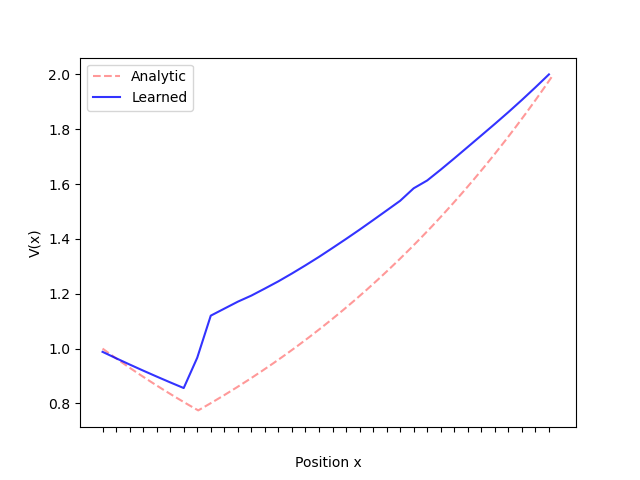
\includegraphics[scale=\munosvaluecomparisonscale]{results/dt-munos-value}
  \end{minipage}%
  \begin{minipage}[h]{0.49\linewidth}
    \centering\textsc{Finite Differences}\\
    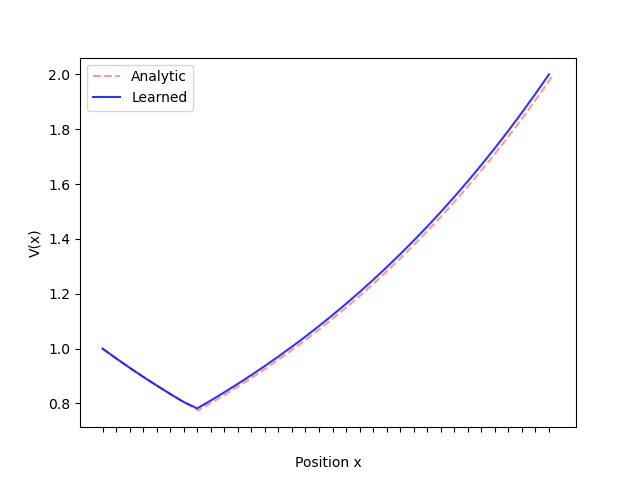
\includegraphics[scale=\munosvaluecomparisonscale]{results/ct-munos-value}
  \end{minipage}
  \caption[Failure of Q-learning in continuous time]{Value functions
    learned by a continuous-time RL algorithm and Q-Learning for
    Munos' toy example}
  \label{fig:munos:value:comparison}
\end{figure}

In our experiments, we use a small timestep duration $\tau=10^{-3}$
and we discretize the state space uniformly into $100$
bins. Hyper-parameter search for the optimal learning rate sequence
was conducted identically for both algorithms. We see that
$Q$-learning converged to a value function with a discontinuity near
the point of non-differentiability of the value function. Consequently
the value function learned by $Q$-learning is only approximately
correct near the boundaries of the state space. On the other hand, the
algorithm with continuous-time corrections learns a continuous value
function that approximates the viscosity solution of
\eqref{eq:dynamic-programming} well on the entire state space.

Beyond this simple environment, \citet{doya2000reinforcement} presents
a number of algorithms that are extensions of existing (discrete-time)
RL algorithms to the continuous time setting, including a method with
differential updates based on the gradient of the value function, and
encorporating $\text{TD}(\lambda)$ updates \citep{sutton1988learning}
to reduce bias. This algorithm was reported to have learned optimal
controllers for complex control tasks faster than discrete-time
counterparts by a substantial amount.

\subsection{Unveiling Problems in Discrete Reinforcement Learning}
Another reason for studying reinforcement learning in the
continuous-time setting is that it forces us to recognize some of the
technical challenges of reinforcement learning that are obscured, but
still present, in the discrete-time MDP model. One such example is 
part of the credit assignment problem, which is the problem of
determining which actions from a given episode in an MDP contributed
most to the return. This problem is certainly addressed in the
reinforcement learning literature \citep{sutton1984temporal,
  arumugam2021information}, however the study of reinforcement
learning in continuous time demonstrates a new challenge.

The work of \citet{baird1993advantage} presents an interesting
challenge for credit assignment when the timestep is small (or
infinitesimal). For systems evolving continuously in time, we expect
different controls to have similar $Q$-values at a given state -- that
is, individual actions should not perturb the overall return too
greatly. In fact, it is shown in \citet{baird1993advantage} and
formally proved in \citet{tallec2019making} that as
the timestep shrinks, the $Q$-function may completely disregard the
action altogether. In that case, $Q$-learning at the very least should
be expected to learn extremely slowly, if at all. In order to correct
this, the \emph{Advantage Updating} algorithm is presented, where
``advantage'' functions are learned as opposed to $Q$-functions, and
the advantage functions $A$ are related to the $Q$-functions via

\begin{equation}
  \label{eq:advantage-updating}
  A(x, a) = \frac{1}{\tau}\left(Q(x, a) - \max_{a'\in\mathcal{A}}Q(x, a')\right)
\end{equation}

where $\tau$ is the duration of the timestep. By effectively scaling
$Q$-functions by $\tau^{-1}$, the advantage functions do not lose
information about actions in the continuous time limit, and
\citet{baird1994reinforcement} reports that advantage learning
converged $10^5$ times faster than $Q$-learning in their
experiments. The work of \citet{bellemare2016increasing} develops
further on this idea by demonstrating a class of ``consistent''
Bellman-like operators, and empirical results in complex experiments
using consistent updates substantially improve over previous similar
RL algorithms.

Another approach to solving the continuous-time credit assignment
problem was recently suggested by \citet{kim2021hamilton}, which
presents the Hamilton-Jacobi Deep Q Network (HJ-DQN). This framework
allows us to perform value-based RL when the action space is
continuous, under the assumption that the control signal is
Lipschitz-continuous in time. This assumption effectively means that
the control is not changing too quickly, so the individual controls
have more influence on the final return. Moreover, by the definition
of Lipschitz-continuity, the time-derivative of the control signal is
bounded by some constant $L$ and we can determine the optimal action
at each timestep (even though there are infinitely many candidates!)
by

\begin{align*}
  \dot{a}(t) &= L\frac{\nabla_aQ(x, a)}{\|\nabla_a Q(x, a)\|}
\end{align*}

Simply put -- we must determine the direction in action space that
maximizes the $Q$-function most quickly by computing the $a$-gradient
of the $Q$ function, and then perturb the control as much as we're
allowed to by the Lipschitz constraint in that direction.

A similar feat can be accomplished if we make an alternative
assumption that the dynamics are \emph{control-affine}, meaning
$\dot{x}(t) = f(x(t)) + \langle g, a(t)\rangle$ for some linear
operator $g$ and arbitrary function $f$. In particular, under this
class of dynamics, value-maximizing actions can be computed in closed
form even when the action space is uncountable
\citep{tassa2007least}. Recently, this idea was applied with great
success in the Continuous Fitted Value Iteration (cFVI) algorithm
\citep{lutter2021value} and in the Robust Fitted Value Iteration
(rFVI) algorithm \citep{lutter2021continuous}. 

The study of \citet{tallec2019making} also discusses what is a
seemingly un-explored parameter of reinforcement learning models: the
length of the timestep. Even when the timesteps are not miniscule, it
is not unreasonable to suspect that RL algorithms might perform
differently due to changes in the timestep length. In fact, their work
shows that existing discrete-time value-based RL algorithms are quite sensitive to
the time discretization parameter, while continuous-time RL algorithms
tend to be much more stable. This on its own demonstrates the
importance of studying RL in the continuous-time limit.

\subsection{The Stochastic Case}
Continuous-time optimal control of a system governed by stochastic
dynamics has been thoroughly studied \citep{fleming2006controlled}. In
most of the literature, the Markov processes underlying the evolution
of the system are assumed to be \hyperref[s:ito-diffusion]{\Ito\
Diffusions} (shown in \S\ref{s:ito-diffusion}), and this will be the case in the
remainder of this thesis as well.

In the stochastic control setting, the HJB equation is not quite the
same as \eqref{eq:dynamic-programming} -- this is mainly due to the
extra second-order term that emerges by \hyperref[app:ito]{\Ito's
lemma}, shown in \eqref{eq:ito}. Deriving the corresponding equation, however,
can be done trivially by exploiting \hyperref[app:feynman-kac]{the Feynman-Kac
formula}, shown in Appendix \ref{app:feynman-kac}. Simply by observation, for
any fixed policy $\pi$ we have

\begin{align*}
  V^\pi(x) &= \ConditionExpect{\int_0^\infty\gamma^tr(X_t,
             A_t)dt}{X_0=x, A_t\sim\pi(\cdot\mid X_t)}
\end{align*}

According to the Feynman-Kac formula, this is the exact form of the
solution to the PDE

\begin{equation}
  \label{eq:hjb:stochastic}
  0 = \langle\nabla_xV^\pi(x), f_\pi(x)\rangle +
  \frac{1}{2}\trace\left(\quadraticform{\pmb{\sigma}_\pi(x)}{\hessian{x}V^\pi(x)}\right)
  + V^\pi(x)\log\gamma
\end{equation}

where the state process $\indexedabove{t}{X}$ is governed by the \Ito\
diffusion

\begin{align*}
  dX_t = f_\pi(X_t, A_t)dt + \pmb{\sigma}_\pi(X_t)dB_t.
\end{align*}

Existing continuous-time reinforcement learning algorithms have been
adapted to account for \eqref{eq:hjb:stochastic}. A great example is
the algorithm introduced in \citet{munos1997reinforcement}, which
extends the finite differences algorithm from \citet{Munos2004ASO} by
deriving a finite differences scheme to account for the second order
term
$\quadraticform{\pmb{\sigma}_\pi(X_t)}{\hessian{x}V^\pi(x)}$. More
recently, stochastic control algorithms with powerful function
approximation have been studied, using techniques such as the
construction of forward-backward SDEs to allow for efficient
backpropagation \citep{pereira2019learning} and importance sampling via
\hyperref[thm:girsanov]{Girsanov's theorem} to accounting for
off-policy learning \citep{exarchos2018stochastic}.

\section{Distributional Reinforcement Learning}\label{s:distributional-rl}
In many applications of machine learning, it is desirable to
understand the uncertainty involved in predictions from a model. For
instance, in robotics applications it is usually a good idea to use
knowledge of uncertainty to provide safety margins in order to prevent
serious damages, and in clustering algorithms we can assign to each
datapoint a distribution over possible categories. The young field of
distributional reinforcement learning takes uncertainty modeling to
the core object of interest in value-based RL: the value function itself.

More formally, the idea behind distributional RL is to model the
probability distribution of random returns as opposed to just its
expected value. While this idea may seem innocuous at first glance, estimating
return distributions presents a plethora of mathematical challenges.

Recall that a popular technique for learning the value function in RL
is to derive a \hyperref[def:contraction]{contractive operator} on the
space of value functions and invoke the
\hyperref[thm:banach-fixed-point]{Banach fixed-point theorem} to prove
that repeated applications of this operator will yield the value
function. Already, to bridge this technique to the distributional
framework, we are immediately faced with problems that must be addressed:

\begin{enumerate}
\item Can the return distribution function be expressed as the fixed point of
  an operator?
\item What is a contraction on the space of probability measures, and
  in particular, what does it mean for probability measures to be
  close to each other?
\item What is an \emph{optimal} return distribution function?
\end{enumerate}

In the seminal work of \citet{Bellemare2017ADP}, some of these
questions are answered. By extending the results concerning analysis
of fixed points on the space of distributions due to
\citet{rosler1992fixed}, \citet{Bellemare2017ADP} shows that the
return distribution does indeed satisfy a fixed-point equation for a
distributional extension of the Bellman operator. However, in order to
satisfy a fixed point equation of any kind, we must be clear about the
\hyperref[def:metric-space]{metric space} that we are analyzing. As it
turns out, the distributional Bellman operator is not contractive for
several familiar topologies on the space of probability measures
\citep{Bellemare2017ADP}, such as the total variation distance and the
Kullback-Leibler (KL) divergence\footnote{The KL divergence is
  actually not a metric, as it is not symmetric. However, there are
  many ways to construct metrics out of the KL divergence that
  preserve its properties.}.

An illustrative example of this, inspired by an example given by Professor
Prakash Panangaden in a talk at Mila, is as follows. Suppose there
exists a state $x$ in an MDP for which the return is deterministically
some number $y$, so
its return distribution is $\returnmeasure(\cdot\mid x) =
\dirac{y}$. Let's say we're estimating this distribution by a
distribution $\mu(\cdot\mid x) = \dirac{z}$. As long as $z\neq y$, the
total variation distance between $\mu(\cdot\mid x)$ and
$\returnmeasure(\cdot\mid x)$ is given by

\begin{align*}
  \text{TV}(\mu,\returnmeasure)\triangleq\frac{1}{2}\sup_{A\in\mathcal{F}}\left\lvert
  \mu(A\mid x) - \returnmeasure(A\mid x)\right\rvert = 1
\end{align*}

where $\mathcal{F}$ is the $\sigma$-algebra associated with the
measurable space of interest. Notably, regardless of how far $z$ is
from $y$ (note that this notion of distance is familiar, since
$y,z\in\mathbf{R}$), the learning signal according to the total
variation distance is always $1$! That is, total variation distance
would tell us that the probability distributions $\dirac{1.0001}$ and
$\dirac{10^7}$ are equidistant from $\dirac{1}$, for example. Clearly,
this does not capture the notion of similarity between probability distributions
that we expect in reinforcement learning.

An insight from the previous example is that the notion of distance
between probability measures in $\probset{\mathcal{W}}$ should be
related in some way to the topology of $\mathcal{W}$. This is captured
nicely by the \emph{Wasserstein distances} \citep{villani2008optimal}.

\begin{definition}[Wasserstein distance]\label{def:wasserstein}
  Let $(\mathcal{W}, d)$ be a metric space and $(\mathcal{W},
  \mathcal{F})$ a measurable space over which $\mu,\nu$ are
  measures. A (probabilistic) \textbf{coupling} between $\mu,\nu$ is a
  probability measure $\pi$ on the product space
  $\mathcal{W}\times\mathcal{W}$ such that $\mu =
  \pushforward{(\identity, \mathcal{W})}{\pi}$ and
  $\nu=\pushforward{(\mathcal{X}, \identity)}{\pi}$ -- that is, the
  marginals of $\pi$ are $\mu,\nu$ respectively.

  Suppose $\mathcal{W}$ is a normed space, and let $\Pi$ denote the
  set of all couplings of measures in $\probset{\mathcal{W}}$. For $p\in\{1,\dots,\}$, the
  $p$-\textbf{Wasserstein distance} $\wassermetric[p]$ is defined as

  \begin{align*}
    \wassermetric[p](\mu,\nu) &=
                                \min_{\pi\in\Pi}\left(\int_{\mathcal{W}\times\mathcal{W}}\|x
                                - y\|^pd\pi(x, y)\right)^{1/p}
  \end{align*}

  Note that the ``optimal coupling'' satisfying the minimization above
  always exists, and $\wassermetric[p]$ is a metric over
  $\probset{\mathcal{W}}$ \citep{villani2008optimal}. 

  The metric space $(\probset{\mathcal{W}}, \wassermetric[p])$ is denoted by
  $\wassersteinspace[p]{\mathcal{W}}$.
\end{definition}

In the notation of \citet{Rowland48495}, \citet{Bellemare2017ADP}
shows that the \emph{distributional} Bellman operator
$\bellmanoperator:\probset{\mathbf{R}}\to\probset{\mathbf{R}}$
defined as

\begin{align*}
  \bellmanoperator\returnmeasure(\cdot\mid x, a) &=
                                                       \Expectation{x'\sim
                                                       P(\cdot\mid x,
                                                       a)\atop
                                                       a'\sim\pi(\cdot\mid
                                                       x')}{\pushforward{f^{r,
                                                       \gamma}}{\returnmeasure(\cdot\mid
                                                       x', a')}}\\
  f^{r, \gamma}(\xi) &= r + \gamma\xi,
\end{align*}

is a contraction in a ``supremal form'' $\supremalwassermetric[p]$
of the $p$-Wasserstein metric,

\begin{align*}
  \supremalwassermetric[p](\mu, \nu) &= \sup_{x\in\mathcal{X}\atop
                                          a\in\mathcal{A}}\wassermetric[p](\mu(\cdot\mid
                                          x, a),\nu(\cdot\mid x, a)).
\end{align*}

In the same work, it is shown that $\supremalwassermetric[p]$ is
indeed a metric on the space of functions with the type signature
$\mathcal{X}\times\mathcal{A}\to\probset{\mathbf{R}}$.

At the time, there was no known, tractable method for computing
gradients of Wasserstein distances from samples
\citep{bellemare2017cramer}, so consequently the C51 algorithm
presented in \citet{Bellemare2017ADP} worked by backpropagating
gradients of the KL divergence, despite the negative theoretical
results. C51 was tremendously successful, and to this day it
contributes positively to state of the art deep reinforcement learning
models \citep{hessel2018rainbow}.

Soon after, \citet{Dabney2018DistributionalRL} discovered a method for
minimizing the
$1$-Wasserstein metric from samples by exploiting a property of Wasserstein
distances over the reals \citep[Theorem 2.1]{thorpeintroduction} and
performing quantile regression \citep{koenker1978regression}. This
resulted in another exceptional deep RL algorithm, known as QR-DQN,
which also maintains its presence in state of the art models
\citep{bellemare2020autonomous}.

Following this, \citet{Rowland48495} constructs a framework for proper
return distribution learning by distinguishing return distribution
samples from return distribution statistics. In this work, methods
of representing probability measures as functions of their statistics
are characterized according to how well they can approximate fixed
points of certain distributional operators, including the
distributional Bellman operator. This analysis partly explains the
great empirical performance of C51 given its deviation from the theory
of distributional RL.

There have since been many developments in distributional RL
concerning representations of the return distributions, as will be
discussed later in \S\ref{s:representation}. Additionally,
distributional RL has been studied as a tool for promoting exploration
in RL \citep{mavrin2019distributional} as well as \emph{safe}
exploration \citep{zhang2021safe}.

Aside from the contributions of this thesis, distributional RL in
continuous time has only been studied by the concurrent work of
\citet{halperin2021distributional}, which focuses mainly on
risk-sensitive RL in continuous time and provides no algorithms for
learning return distribution functions.

\section{Gradient Flows in Abstract Metric Spaces}\label{s:gradient-flows}
This section will delve into a formalism for studying certain iterative
refinement algorithms in the limit as the iterations occur continuously in time.
In Chapter \ref{c:approximate-dp}, we will use this formalism to describe a
continuous-time extension of \hyperref[eq:policy-evaluation]{policy evaluation}.
We will make extensive use of the topological concepts of Appendix
\ref{app:analysis}, particularly \S\ref{s:metric-space} where metric spaces are
defined. More in-depth treatments of the topics in this section can be found in
\citet{ambrosio2008gradient}, \citet{santambrogio2015optimal}, and
\citet{villani2008optimal}.

As we saw in \S\ref{s:background:rl:contraction}, a common approach to solving
the Bellman equation is by iteratively applying an operator to an initial guess
of the value function until a fixed point is reached. However, such an iterative
method is a discrete-time operation by its very nature. When developing
continuous-time RL algorithms later in the thesis, we will look at the
``continuous-time" limit of such an iterative algorithm. Purely for the sake of
building intuition, we can think of this continuous-time limit as a solution to
the \emph{Cauchy problem}\citep{ambrosio2008gradient},

\begin{equation}\label{eq:cauchy-problem}
  \begin{cases}
    \partialderiv{}{t}v(t, \cdot) = -\nabla\mathscr{F}(v(t, \cdot))\\
    v(0, x) = V_0(x)
  \end{cases}
\end{equation}

where $v(t, \cdot)\in\mathcal{V}$ represents the estimate of the value
function at time $t$ among the class of value functions $\mathcal{V}$,
$\mathscr{F}:\mathcal{V}\to\mathbf{R}$ is a \emph{loss functional}, and
$V_0\in\mathcal{V}$ is the initial guess of the value function. In Q-Learning,
we update estimates of the Q-function so as to minimize the squared error
between $Q$ and $\mathscr{T}Q$, so we may interpret \eqref{eq:cauchy-problem} as
a continuous-time process during which the value function $v(t, \cdot)$ moves
in the direction of the steepest descent of the error signal it incurs. More
succinctly, this represents a continuous-time extension of gradient descent,
which is called a \emph{gradient flow}.

However, in a general metric space, the Cauchy problem has no meaning, and
consequently we must consider an alternative formulation in order to make sense
of the Cauchy problem in spaces without much algebraic structure. If we look
more closely at \eqref{eq:cauchy-problem}, we note that
neither of its two terms have any proper meaning when $\mathcal{V}$ is an
arbitrary metric space \citep{ambrosio2008gradient}.
Indeed, the familiar definition of the time derivative
would be expressed as $\partialderiv{}{t}v(t, \cdot) = \lim_{\delta\to
0}\frac{1}{\delta}(v(t + \delta, \cdot) - v(t, \cdot))$, and this requires
that $\mathcal{V}$ is closed under an invertible, associative binary operation
as well as scalar multiplication
(i.e, $\mathcal{V}$ should be a vector space). This condition of course is not
satisfied when it is only assumed that $\mathcal{V}$ is a metric space.

While such an issue may seem like an unnecessary technicality, it most certainly
is not. A relevant example that demonstrates why this abstraction is necessary
is when $\mathcal{V}$ is a space of return distribution functions. One must be
very careful when performing algebraic operations on such objects -- most often
return distribution functions \emph{do not} form a vector space. Suppose
$\eta\in\mathcal{V}$ and $|\alpha|\neq 1$. Then since $\eta(\returnspace\mid x)
= 1$ by definition, we must have $\alpha\eta(\returnspace\mid x)\neq 1$, so
$\alpha\eta$ is not a probability measure, and it follows that $\mathcal{V}$ is
not closed under scalar multiplication. Thus, certainly for the purpose of this
thesis, we must study an abstraction of gradient flows to general metric spaces.

\subsection{Evolution Variational Inequality}\label{s:gradient-flows:evi}
A clever way to deal with generalizing the gradient flow formulation involves
expressing the gradient flow in a simple metric space (say, a Hilbert space) by
an equivalent identity comprised solely of metric operations. Since the
resulting expression is equivalent to a gradient flow, it provides a meaningful
notion of a gradient flow in spaces that don't necessary have a vector space
structure. Generally, this
requires invoking assumptions on $\mathscr{F}$.

A very useful characterization is known as an \emph{evolution variational
inequality} \citep{de1980problems}. We begin by assuming that $\mathcal{V}$ is a
Hilbert space and $\mathscr{F}$ is
$\lambda$-convex \citep{santambrogio2015optimal}, meaning that for every
$\psi\in\mathcal{V}$, we have

\begin{align*}
  \mathscr{F}(\psi) &\geq \mathscr{F}(\phi(t)) + \frac{\lambda}{2}\|\phi(t) - \psi\|^2 +
  \langle p, \psi - \phi(t)\rangle
\end{align*}

where $\phi:\mathbf{R}_+\to\mathcal{V}$ and $p$ is in the subdifferential of
$\mathscr{F}$ evaluated at $\phi(t)$. If $\phi$ is a solution to the Cauchy
problem \eqref{eq:cauchy-problem}, then $p = -\partialderiv{}{t}\phi(t)$. It
follows that

\begin{align*}
  \mathscr{F}(\psi) &\geq \mathscr{F}(\phi(t)) + \frac{\lambda}{2}\langle\phi(t) -
  \psi, \phi(t) - \psi\rangle - \langle \phi'(t), \psi - \phi(t)\rangle\\
\end{align*}

Moreover, note that

\begin{align*}
  \frac{1}{2}\partialderiv{}{t}\|\phi(t) - \psi\|^2 &=
  \left\langle\partialderiv{}{t}(\phi(t) - \psi), \phi(t) - \psi\right\rangle\\
                                                    &=
                                                    \left\langle\partialderiv{}{t}\phi(t),
                                                      \phi(t) -
                                                      \psi\right\rangle\\
\end{align*}

So, when $\mathscr{F}$ is $\lambda$-convex and $\phi$ solves the Cauchy problem,
we have

\begin{align*}
  \mathscr{F}(\psi) &\geq\mathscr{F}(\phi(t)) + \frac{\lambda}{2}\|\phi(t) -
  \psi\|^2 + \frac{1}{2}\partialderiv{}{t}\|\phi(t) - \psi\|^2\\
\end{align*}

Finally, noting that $\|x - y\|^2 = d^2(x, y)$ where $d$ is the metric in the
Hilbert space $\mathcal{V}$, we have

\begin{equation}\label{eq:evi:def}
  \frac{1}{2}d^2(\phi(t), \psi) \leq \mathscr{F}(\psi) - \mathscr{F}(\phi(t)) -
  \frac{\lambda}{2}d^2(\phi(t), \psi)
\end{equation}

Equation \eqref{eq:evi:def} is known as the $\text{EVI}_\lambda$ inequality.
Note that this inequality is expressed only in terms of metric quantities, so it
is a suitable characterization of a gradient flow in abstract metric space as
long as the concept of $\lambda$-convexity can also be defined in terms of
metric quantities. Fortunately, it is known \citep{muratori2018gradient} that
$\mathscr{F}$ is $\lambda$-convex if and only if
for every
$\phi,\psi\in\mathcal{V}$ there exists a geodesic\footnote{A geodesic between
  two points is a curve between those points for which the arc length of the
  curve according to the space's metric is minimal.}
$\indexedin{[0,1]}{t}{\varrho}$ with $\varrho_0 = \phi$ and $\varrho_1=\psi$
such that

\begin{equation}\label{eq:lambda-convex:metric}
  \mathscr{F}(\varrho_t) \leq (1 - t)\mathscr{F}(\phi) + t\mathscr{F}(\psi) -
  \frac{\lambda}{2}t(1 - t)d^2(\phi, \psi)
\end{equation}

Note that when $\lambda>0$, which we generally desire, $\lambda$-convexity is a
stronger property than convexity. Hence, we will consider the following
characterization of gradient flows.

\begin{definition}[Abstract Gradient Flow]\label{def:abstract-gradient-flow}
  Let $(\mathcal{V}, d)$ be a metric space, and let
  $\phi:\mathbf{R}_+\to\mathcal{V}$ be a curve in $\mathcal{V}$. If
  $\mathcal{F}$ is $\lambda$-convex in the sense of
  \eqref{eq:lambda-convex:metric} and
  $\phi$ satisties the $\text{EVI}_\lambda$ inequality \eqref{eq:evi:def}, then
  $\phi$ is said to be a (EVI-type) \textbf{gradient flow} of $\mathscr{F}$.
\end{definition}

An attractive property of EVI-type gradient flows is that they satisfy a
contraction property, which will play an analogous role to
\hyperref[s:background:rl:contraction]{contraction mappings} in discrete-time
analysis. This suggests that EVI-type gradient flows are a promising candidate
for describing continuous-time policy evaluation.

\begin{theorem}[Uniqueness of Gradient Flows, \citep{santambrogio2015optimal}]
  Let $(\mathcal{V}, d)$ be a metric space. If two curves $\phi,\varphi :
  \mathbf{R}_+\to\mathcal{V}$ satisfy the $\text{EVI}_\lambda$ inequality
  \eqref{eq:evi:def} for some $\lambda\geq 0$ and a $\lambda$-convex functional
  $\mathscr{F}$, then
  \begin{align*}
    \frac{d}{dt}d^2(\phi(t), \varphi(t))\leq -2\lambda d(\phi(t), \varphi(t))
  \end{align*}

  Then, by Gr\"onwall's lemma \citep{gronwall1919note}, it follows that

  \begin{align*}
    d(\phi(t), \varphi(t)) \leq e^{-\lambda t}d(\phi(0), \varphi(0))
  \end{align*}
\end{theorem}

This shows that any two EVI-type gradient flows for a common $\lambda$-convex
loss functional will eventually coincide. Consequently, if continuous-time
policy evaluation can be framed as an EVI-type gradient flow, we can be assured
that the continuous-time policy evaluation process will converge to a unique
fixed point (say, the return distribution function). The work of
\citet{martin2019stochastically} exploits this concept to formulate
distributional policy evaluation of a discrete-time process as an EVI-type
gradient flow, and we will develop this idea further in Chapter
\ref{c:approximate-dp} for continuous-time policy evaluation.

\subsection{Wasserstein Gradient Flows}\label{s:gradient-flows:wgf}
In \S\ref{s:distributional-rl} we defined the
\hyperref[def:wasserstein]{Wasserstein distance} as a convenient distance
measurement between probability measures in distributional RL. It is a beautiful
result from optimal transport theory that the
Wasserstein distances are proper \hyperref[def:metric-space]{metrics} over
spaces of probability measures \citep{villani2008optimal}. For a metric space
$(\mathcal{V}, d)$, the metric space $(\probset{\mathcal{V}},
\wassermetric[p])$ (with $\wassermetric[p]$ having the same definition as in
definition \ref{def:wasserstein}) is called the $p$-Wasserstein space, and it is denoted by
$\wasserspace[p]$.

Among all Wasserstein spaces, the space $\wasserspace$ is by and large the most
convenient for the analysis of smooth curves in the space of probability
measures \citep{Santambrogio2016EuclideanMA}. For this reason, the analysis of
gradient flows in probability measure space is often conducted in $\wasserspace$,
and the term \emph{Wasserstein Gradient Flow} (WGF) almost exclusively refers to
gradient flows in $\wasserspace$ specifically.

Perhaps the most celebrated result in the study of WGFs is that of Jordan,
Kinderlehrer, and Otto \citep{Jordan02thevariational}, known as the JKO scheme.
As an overview, the result is comprised of the following points:

\begin{enumerate}
  \item The \textbf{Fokker-Planck} equation, which is a widely studied PDE in
    physics and is given by

    \begin{equation}\label{eq:fokker-planck}\tag{FP}
      \partialderiv{}{t}\varrho(t, x) = -\partialderiv{}{x}\left(\mu(x,
        t)\varrho(x, t)\right) + \frac{\partial^2}{\partial
      x^2}\left(\sigma^2(t, x)\varrho(t, x)\right)
    \end{equation}

    where $\mu,\sigma$ are known and $\sigma$ is positive definite, satisfies
    the \textbf{continuity equation}

    \begin{equation}\label{eq:continuity-equation}\tag{CE}
      \partialderiv{}{t}\varrho(t, x) + \nabla_x\cdot(\varrho(t, x)\mathbf{v}(t,
      x)) = 0
    \end{equation}

    for some vector field $\mathbf{v}$, which characterizes the conservation of
    mass of the process $\varrho$. If we think of $\varrho(t, \cdot)$ as a
    probability density, this means that we can interpret
    \eqref{eq:fokker-planck} as an equation governing the evolution of a
    probability density that conserves measure.
  \item The Fokker-Planck equation \eqref{eq:fokker-planck} for a constant
    $\sigma$ is the
    \textbf{Cauchy problem} associated to the \textbf{Wasserstein gradient flow}
    of the functional $\mathscr{F}$ given by

    \begin{equation}\label{eq:fokker-planck:wgf}\tag{FPWGF}
      \mathscr{F}(\varrho(t,\cdot)) = \int_{\mathcal{X}}U(x)\varrho(t, dx) -
      \sigma\mathcal{H}(\varrho(t,\cdot))
    \end{equation}

    where $\mathbf{v}(t, x) = -\nabla U(x)$.

  \item The loss functional \eqref{eq:fokker-planck:wgf} can equivalently be
    written as $\mathscr{F}(\varrho(t, \cdot)) = \kl{\varrho(t, \cdot)}{\mu}$ where

    \begin{align*}
      \mu(x) &= \frac{1}{Z}e^{-U(x)}\\
      Z &\triangleq\int_{\mathcal{X}}e^{-U(x)}dx
    \end{align*}

    Thus, the Fokker-Planck equation can be interpreted as the evolution of
    a probability density towards $\mu$ in the sense of KL divergence.
    Naturally, it follows that $\mu$ is the stationary solution of
    \eqref{eq:fokker-planck}.
  \item Following the analysis of \textbf{generalized minimizing movements
      schemes}
    \citep{de1993new}, it is shown that under an appropriate time discretization
    (discussed further in \S\ref{s:policy-evaluation}), for any timestep $\tau$,
    sequences given by

    \begin{align*}
      \varrho^\tau_{k+1} &\in \arg\min_{\nu\in\wasserspace}\left[\mathscr{F}(\nu) +
      \frac{1}{2\tau}\wassermetric^2(\nu, \varrho^\tau_k)\right]
    \end{align*}

    satisfy $\lim_{\tau\to 0}\varrho^\tau_k\to \mu$, where convergence is
    attained with respect to $\wassermetric$. The JKO scheme refers to
    the process of \textbf{approximately solving} \eqref{eq:fokker-planck} by
    \textbf{iteratively}
    computing terms of the sequence $\indexedint{k}{\infty}{\varrho^\tau}$ for
    small $\tau$, where $\varrho^\tau_0$ is an arbitrary probability density.
    Notably, this approximation converges to the true gradient flow as $\tau\to
    0$.
\end{enumerate}

In the context of reinforcement learning, this result is very useful, as it
describes a convergent method to solve a Cauchy problem discretized in time that
is similar to dynamic programming. This will be the focus of
\S\ref{s:policy-evaluation}.

\chapter{Evolution of Return Distributions}\label{c:evolution}
We will now shift our focus to formally representing the return
distribution function for an RL agent evolving continuously in time
with a fixed behavioral policy. In order to do so, it will be
necessary to impose some structural and regularity properties on the
dynamics of the environment and on the return distributions. More concretely,
the chapter is structured as follows,

\begin{itemize}
  \item A formalism of \textbf{continuous-time Markov processes} will be given;
  \item The \textbf{random return} is formulated as a \textbf{special type of
    Markovian process} in \S\ref{s:truncated-returns};
  \item A \textbf{distributional analogue to the HJB equation} (see
    equation \eqref{eq:hjb:stochastic}) is derived in \S\ref{s:characterization}.
\end{itemize}

In order to model stochastic trajectories in continuous time, we will use the
language of stochastic processes and stochastic differential equations as
discussed in \S\ref{s:stochastic-processes} and Appendix \ref{app:stochastic}.
Moreover, we must discuss what it means for a continuous-time process to be
Markovian.

\begin{definition}[Markov Process,
  \cite{rogers1994diffusions}]\label{def:transition-semigroup}
  Let $(X_t)_{t\geq 0}$ be a stochastic process in the
  \hyperref[def:filtration]{filtered probability space} $(\Omega,
  \mathcal{F}, (\mathcal{F}_t)_{t\geq 0}, \Pr)$. A \emph{Markovian
    transition kernel} is a kernel with a continuous parameter $t$,
  $P_t:\Omega\times\mathcal{F}\to[0,1]$, such that for any bounded
  $\mathcal{F}$-measurable function $f$, we have

  \begin{equation}\label{eq:markov-kernel}
    (P_tf)(X_s) = \ConditionExpect{f(X_{s+t})}{\mathcal{F}_s}\qquad
                                                                  \Pr-\text{almost surely}
  \end{equation}

  A collection $(P_t)_{t\geq 0}$ of Markovian transition kernels is called a
  \emph{transition semigroup}\footnote{This name emphasizes
    the semigroup nature of the collection of transition kernels. In
    the abstract algebra literature, a semigroup is a set of objects that is
  closed under an associative binary operation.} when
  \begin{enumerate}
  \item For each $t\geq 0$ and $x\in\Omega$, $P_t(x,\cdot)$ is a
    measure on $\mathcal{F}$ and $P_t(x,\Omega)\leq 1$;
  \item For each $t\geq 0$ and $\Gamma\in\mathcal{F}$, the mapping
    $P_t(\cdot,\Gamma)$ is $\mathcal{F}$-measurable; and
  \item (The Chapman-Kolmogorov Identity) For each $s,t\geq 0$,each
    $x\in\Omega$, and each $\Gamma\in\mathcal{F}$, the collection
    satisfies

    \begin{align*}
    P_{s+t}(x,
    \Gamma) = \int_\Omega P_s(x, dy)P_t(y, \Gamma)
    \end{align*}
  \end{enumerate}
  Then $P_tP_s = P_{t+s}$, so $\indexedabove{t}{P}$ is indeed a semigroup.

  A \emph{Markov process} is a stochastic process $\indexedabove{t}{X}$ together
  with a transition semigroup $\indexedabove{t}{P}$ such that
  \eqref{eq:markov-kernel} holds.
\end{definition}

Beyond the Markovian property, we will further require that the trajectory of
the agent is ``regular enough" for us to study its instantaneous dynamics. In
particular, we will assume henceforth that the trajectory of the agent is a
\emph{Feller-Dynkin} process.

\begin{definition}[Feller-Dynkin Process, Infinitesimal Generator,
  \cite{rogers1994diffusions}]\label{def:fd}
  Consider a filtered probability space $(\Omega, \mathcal{F},
  (\mathcal{F}_t)_{t\geq 0}, \Pr)$ and let $\mathcal{X}$ be a Polish\footnote{A
    Polish space is a \hyperref[def:complete]{complete}
    \hyperref[def:metric-space]{metric space} that has a countable, dense
    subset.} space. A transition semigroup
  $(P_t)_{t\geq 0}$ is said to be a \emph{Feller semigroup} if
  \begin{enumerate}
  \item $P_t : C_0(\mathcal{X})\to C_0(\mathcal{X})$ for each
    $t\in\mathbf{R}_+$;
  \item For any $f\in C_0(\mathcal{X})$ with $f\leq 1$, $P_tf\in[0,1]$;
  \item $P_sP_t = P_{s+t}$ and $P_0=\identity$;
  \item For any $f\in C_0(\mathcal{X})$, we have
    $\|P_tf-f\|\overset{t\downarrow 0}{\longrightarrow} 0$.
  \end{enumerate}

  A Markov process with a Feller semigroup is called a
  \emph{Feller-Dynkin process}.

  Define the set $\mathscr{D}(\mathscr{L})$ according to

  \begin{align*}
    \mathscr{D}(\mathscr{L}) &= \left\{\Conditional{f\in
                               C_0(\mathcal{X})}{\exists g\in
                               C_0(\mathcal{X})\quad\text{\small such that}\quad \|\delta^{-1}(P_\delta - f)
                               - g\|\overset{\delta\downarrow
                               0}{\longrightarrow} 0}\right\}
  \end{align*}

  The \emph{infinitesimal generator} of a Feller-Dynkin process is the
  operator $\mathscr{L}:\mathscr{D}(\mathscr{L})\to C_0(E)$ where

  \begin{align*}
    \mathscr{L}f = \lim_{\delta\to 0}\frac{P_\delta f - f}{\delta}
  \end{align*}

  and $\mathscr{D}(\mathscr{L})$ is called the \emph{domain of the
    infinitesimal generator} $\mathscr{L}$.
\end{definition}

\begin{remark}
  Note that \hyperref[def:ito-diffusion]{\Ito\ diffusions} with
  Lipschitz-continuous coefficients are Feller-Dynkin processes
  \citep{le2016brownian}.
\end{remark}

We consider a continuous-time MDP $(\mathcal{X}, \mathcal{A}, r,
(P_t), \gamma)$ where $\mathcal{X}\subset\mathbf{R}^d$ is compact,
$(P_t)$ is a Feller semigroup with infinitesimal generator
$\mathscr{L}$, $r: \mathcal{X}\to\rewardspace\subset\mathbf{R}$, and
$\gamma\in(0,1)$. Additionally, we impose a mild assumption on the reward
function.

\begin{assumption}\label{ass:method:bounded-rewards}
  The range $\rewardspace$ of $r$ is contained in an
  interval $[R_{\min}, R_{\max}]$, where $|R_{\min}|,|R_{\max}| <\infty$.
\end{assumption}

When assumption \ref{ass:method:bounded-rewards} is satisfied, we make
the following observations regarding the extrema of the return,

\begin{equation*}
  \begin{aligned}
    \returnfunction(x) &= \Conditional{\int_0^\infty\gamma^tr(X_t)dt}{X_0 = x}\\
    V_{\min}\triangleq\inf \returnfunction(x)&\geq\int_0^\infty\gamma^tR_{\min}dt\\
    &= \frac{1}{\log\frac{1}{\gamma}}R_{\min}\\
    V_{\max}\triangleq\sup \returnfunction(x)&\leq\int_0^\infty\gamma^tR_{\max}dt\\
    &= \frac{1}{\log\frac{1}{\gamma}}R_{\max}\\
  \end{aligned}
\end{equation*}

This confirms that the discounted return will be bounded. We refer to
the set $\mathcal{R} = [V_{\min}, V_{\max}]$ as the \emph{return
  space}.

In order to give a formal treatment of the stochastic processes
generated by the agent interacting with its environment, we must
specify a \hyperref[def:filtration]{filtration}.
In particular, we will be interested for the most part in
the \label{def:canonical-filtration}\textbf{canonical filtration}. The
canonical filtration is the filtration $\indexedabove{t}{\mathcal{F}}$
where $\mathcal{F}_t$ is the sub-$\sigma$-algebra generated by the
trajectory observed up to time $t$. Naturally,
$\mathcal{F}_t\subset\mathcal{F}_{t+\delta}$ for any $\delta>0$.

We will perform analysis of the continuous-time MDP on a filtered
probability space \label{def:probability-space}$\mathsf{P} = (\Omega,
\mathcal{F}, (\mathcal{F}_t), \Pr)$, where 
\begin{itemize}
\item $\Omega \subset
  \cup_{n\geq 0}(\mathbf{R}_+\times\mathcal{X}\times\mathcal{A}\times\rewardspace)^n$ is
  the sample space of trajectories in the MDP;
\item $\mathcal{F}$ is a $\sigma$-algebra over $\Omega$;
\item $\indexedabove{t}{\mathcal{F}}$ is the canonical filtration.
\end{itemize}

We denote by $\returnmeasure^\pi:\mathcal{X}\to\probset{\mathcal{A}}$ the
\emph{return distribution function}, which is defined via

\begin{align*}
  \law{G^\pi_x} &= \returnmeasure^\pi(\cdot\mid x),
\end{align*}

where $G^\pi_x$ is the random variable representing the discounted return
obtained by an agent starting at state $x\in \mathcal{X}$ and following a policy
$\pi$. The objects $\returnmeasure^\pi(\cdot\mid x)$ are understood as
\hyperref[def:probability]{probability measures}. We will also require some
assumptions on the regularity of the return distribution function, which are
stated below.

\begin{assumption}
  \label{ass:method:density}
  At every state $x\in\mathcal{X}$, the return distribution
  $\returnmeasure^\pi(\cdot\mid x)$ is absolutely continuous (as a measure over
  the return space) with respect to the
  Lebesgue measure.
\end{assumption}
\begin{assumption}
  \label{ass:method:c2}
  The return distribution function is twice differentiable over
  $\mathcal{X}\times\mathcal{R}$ almost everywhere, and its second
  partial derivatives are continuous almost everywhere.
\end{assumption}

Furthermore, we will occasionally want to analyze some less abstract Markov
processes. In these cases, we will refer to the following assumption.

\begin{assumption}[Diffusion dynamics]
  \label{ass:method:ito-diffusion}
  The Markov process $\indexedabove{t}{X}\subset\mathcal{X}\subset\mathbf{R}^d$
  induced by the agent
  following a fixed (stochastic) policy $\pi$ is an
  \hyperref[def:ito-diffusion]{\Ito\ diffusion} evolving
  according to

  \begin{equation}
    \label{eq:method:ito-diffusion}
    dX_t = f_\pi(X_t)dt + \pmb{\sigma}_\pi(X_t)dB_t
  \end{equation}
  where $f_\pi:\mathcal{X}\to\mathcal{X}$,
  $\pmb{\sigma}_\pi:\mathcal{X}\to\mathbf{R}^{d\times d}$ are
  Lipschitz-continuous, 
  $\pmb{\sigma}_\pi$ is positive semidefinite, and $B_t$ is a
  Brownian motion.
\end{assumption}

\section{The Stochastic Process of Truncated Returns}\label{s:truncated-returns}
We would like to understand how estimates of the random return should
evolve over time. Unfortunately, a function mapping states to (random)
returns cannot be progressively measurable, as it requires knowledge
of an entire trajectory to be computed. Therefore, we will not be able
to study random returns directly with the machinery of stochastic
calculus. Instead, we'll introduce another stochastic process as a
``gateway'' to the random return.

\begin{definition}[The Truncated Return Process]\label{def:truncated-return}
  Let $(\mathcal{X},\mathcal{A},r,(P_t),\gamma)$ be a continuous-time
  MDP. The \emph{truncated return process} is a stochastic process
  $(J_t)_{t\geq 0}\in\mathcal{X}\times\mathcal{R}$ given by

  \begin{equation*}
    \begin{aligned}
      J_t = (X_t, \overline{G}_t)\qquad\overline{G}_t = \int_0^t\gamma^sr(X_s)ds
    \end{aligned}
  \end{equation*}

  The values $\overline{G}_t$ are simply the discounted rewards
  accumulated up to time $t$, and $\overline{G}_0\equiv 0$.
\end{definition}

\begin{proposition}\label{pro:markov}
  The truncated return process $(J_t)_{t\geq 0}$ is a Markov process
  with respect to \hyperref[def:canonical-filtration]{the canonical filtration}.
\end{proposition}
\begin{proof}
  Let $\psi\in C(\mathcal{X}\times\mathcal{R};\mathbf{R})$ and $h>0$. As usual,
  we denote the canonical filtration by $(\mathcal{F}_t)_{t\geq 0}$.
  By the definition of the truncated return process,

  \begin{equation*}
    \begin{aligned}
      \ConditionExpect{\psi(J_{t+h})}{\mathcal{F}_t} &=
      \ConditionExpect{\psi(X_{t+h}, \overline{G}_{t+h})}{\mathcal{F}_t}\\
      &= \ConditionExpect{\psi\left(X_{t+h}, \overline{G}_t + \int_t^{t+h}\gamma^sr(X_s)ds\right)}{\mathcal{F}_t}\\
      &= \ConditionExpect{\psi\left(X_{t+h}, \overline{G}_t + \int_t^{t+h}\gamma^sr(X_s)ds\right)}{J_t}\\
    \end{aligned}
  \end{equation*}

  where the final step holds since the process $(X_t)_{t\geq 0}$ is
  assumed to be Markovian. Thus, we've shown that for any $\psi\in
  C(\mathcal{X}\times\mathcal{R};\mathbf{R})$, there exists a function
  $m:\mathcal{X}\times\mathcal{R}\to\mathbf{R}$ where

  \begin{equation*}
    \ConditionExpect{\psi(J_{t+h})}{\mathcal{F}_t} = m(X_t, \overline{G}_t)
  \end{equation*}

  Therefore, the process $(J_t)_{t\geq 0}$ is Markovian.
\end{proof}

It will be helpful to think of the random return in terms of the
truncated return process. To do so, we'll need to formalize the
concept of a trajectory terminating at a non-deterministic time.

\begin{definition}[Stopping time, \citep{le2016brownian}]\label{def:stopping-time}
  Let $(\Omega, \mathcal{F}, (\mathcal{F}_t))$ be a measurable space
  with \hyperref[def:filtration]{filtration} $(\mathcal{F}_t)$. A random variable
  $T:\Omega\to\mathbf{R}_+$ is called a \emph{stopping time} with
  respect to the filtration $(\mathcal{F}_t)$ if
  \begin{equation*}
    \{T\leq t\} \in\mathcal{F}_t\qquad t\geq 0
  \end{equation*}

  We define the \emph{$\sigma$-algebra of the past before $T$} as the
  $\sigma$-algebra $\mathcal{F}_T$ given by

  \begin{equation*}
    \mathcal{F}_T = \left\{A\in\mathcal{F}_\infty : A\cap\{T\leq t\}\in\mathcal{F}_t\right\}
  \end{equation*}
\end{definition}

Since trajectories are assumed to be Markovian, it is natural to
expect their termination to occur once the agent has reached a state
from some set of \textit{terminating states}. 

\begin{assumption}[Terminating states]\label{ass:termination-set}
  The continuous-time MDP $(\mathcal{X}, \mathcal{A}, r, \indexedabove{t}{P},
  \gamma)$ admits a measurable set $\mathcal{G}\subset \mathcal{X}$, referred to as the
  \emph{terminating states}, such that trajectories terminate when the agent
  reaches any state $x\in \mathcal{G}$.
\end{assumption}

We will confirm that the random termination time corresponding to the first
entry of $\indexedabove{t}{X}$ into $\mathcal{G}$ is a stopping time.

\begin{proposition}\label{pro:stopping-time}
  Consider a \hyperref[def:filtration]{filtered probability space} $(\Omega, \mathcal{F},
  \Pr)$. Let $T$ denote the first time that an agent enters a state among a
  fixed measurable set of terminating states $\mathcal{G}$, so
  \begin{equation*}
    T = \inf_{t\geq 0}\{X_t \in\mathcal{G}\}
  \end{equation*}
  Then if $\mu(T <\infty) = 1$, $T$ is a stopping time with respect to
  \hyperref[def:canonical-filtration]{the canonical filtration}.
\end{proposition}
\begin{proof}
  The proof is simple. For any $\epsilon>0$, there exists
  $t'\in\mathbf{R}$ such that $\Pr(T> t')\leq\epsilon$. Thus,
  with probability at least $1-\epsilon$, $T$ lies in the compact set
  $[0,t']$. Therefore, the function $t\mapsto
  t\indicator{X_t\in\mathcal{G}}$ almost surely attains its
  infimum. Since the characteristic function
  $\omega\mapsto\characteristic{\mathcal{G}}(X_t(\omega)) =
  \indicator{X_t(\omega)\in\mathcal{G}}$ is
  $\mathcal{F}_t$-measurable, it follows that
  $\inf_{t\geq 0}\{T\leq t\}\in\mathcal{F}_t$, so $T$ is a
  stopping time.
\end{proof}

In the remainder of the thesis, we will be interested in the random
(discounted) return $G_x^\pi$ starting at a state
$x\in\mathcal{X}$ and following the policy $\pi$. $G_x^\pi$ is a
random variable due to the fact that the state transitions are
random. We define it as follows,

\begin{equation}
  \label{eq:random-return}
  G_x^\pi = \Conditional{\int_0^T\gamma^tr(X_t)dt}{X_0 = x}
\end{equation}

It's clear that

\begin{equation*}
  \begin{aligned}
    \Conditional{\overline{G}_T \eqlaw G_x^\pi}{X_0=x}
  \end{aligned}
\end{equation*}

The reason for studying the process $(\overline{G}_t)_{t\geq 0}$ as opposed to $G_x^\pi$ is
that $(\overline{G}_t)_{t\geq 0}$ is adapted to the canonical
filtration, whereas $G_x^\pi$ is only measurable with respect to $\mathcal{F}_\infty$.

In temporal difference learning, we perform approximate dynamic
programming to solve the Bellman equation by using the difference
between the value function at a given state and the estimated value
bootstrapped by the value function at the next state as a learning
signal. However, in continuous time, the notion of a ``next state'' is
meaningless. Instead, we study the rate of change of the value
function and approximately solve the resulting PDE. This leaves
another glaring question though: how should one measure or interpret
the rate of change of a noisy (stochastic) signal? To answer this, we
must first introduce some regularity conditions on the dynamics of the
stochastic processes in question.

The following theorem, due to \citet{kolmogoroff1931analytischen}, will be
instrumental in the sequel. A proof is given for clarity.

\begin{theorem}[Kolmogorov Backward Equation]\label{thm:kbe}
  Let $\indexedabove{t}{X}\subset\overline{\mathcal{O}}$ be a Feller-Dynkin
  process for a metric space $\mathcal{O}\subset\mathcal{X}$
  and consider the probability
  space $(\Omega, \mathcal{F}, (\mathcal{F}_t), \Pr)$. Denote by $T$
  the infimum over times $t$ for which $X_t\not\in\mathcal{O}$. For any
  measurable function $\phi$ that is absolutely continuous
  and differentiable almost everywhere, the function $u(x, s) =
  \mathbf{E}[\phi(X_T)\mid X_{s\land T} = x]$ solves the PDE

  \begin{equation}
    \label{eq:kbe}
    \partialderiv{u(x, s)}{s} = -\mathscr{L}u(x, s)
  \end{equation}

  with the terminal condition $u(x, t) = \phi(x)$ when
  $x\in\overline{\mathcal{O}}\setminus\mathcal{O}$, where
  $\mathscr{L}$ is the infinitesimal generator of the process
  $(X_t)_{t\geq 0}$.
\end{theorem}

In order to prove Theorem \ref{thm:kbe}, the following lemma will be
handy.

\begin{lemma}[\citep{le2016brownian}, Theorem 6.14]\label{lem:martingale-generator}
  Let $(X_t)_{t\geq 0}$ be a Feller-Dynkin process on a metric space
  $\mathcal{X}$, and consider functions $h, g\in
  C_0(\mathcal{X})$. The following two conditions are equivalent:
  \begin{enumerate}
  \item $h\in\mathscr{D}(\mathscr{L})$ and $\mathscr{L}h = g$;
  \item For each $x\in\mathcal{X}$, the process
    \begin{equation*}
      \Conditional{h(X_t) - \int_0^tg(X_s)ds}{X_0 = x}
    \end{equation*}
    is a \hyperref[app:martingale]{martingale} with respect to
    the filtration $(\mathcal{F}_t)$.
  \end{enumerate}
\end{lemma}

\begin{proof}[Proof of Theorem \ref{thm:kbe}]
  By Lemma \ref{lem:martingale-generator}, we know that the process
  $\Phi_t = \phi(X_t) -  \int_0^tg(X_s)ds$ is a martingale with
  respect to $(\mathcal{F}_t)$. Let $s<t<T$. By the definition of a
  martingale, we have

  \begin{equation*}
    \small
    \begin{aligned}
      0 = \Expectation{}{\Conditional{\Phi_T}{\mathcal{F}_t}} -
      \Expectation{}{\Conditional{\Phi_T}{\mathcal{F}_s}} &=
    \Expectation{}{\Conditional{h(X_T) +
        \int_0^Tg(X_r)dr}{\mathcal{F}_t}} -
    \Expectation{}{\Conditional{h(X_T) + \int_0^Tg(X_r)dr}{\mathcal{F}_s}}\\
    \Expectation{}{\Conditional{h(X_T)}{\mathcal{F}_t}} -
    \Expectation{}{\Conditional{h(X_T)}{\mathcal{F}_s}} &=
    \Expectation{}{\Conditional{\int_s^t\mathscr{L}h(X_r)dr}{\mathcal{F}_t}}\\
    \end{aligned}
  \end{equation*}

  Dividing through by $t - s$ and taking the limit as $s\uparrow t$,

  \begin{equation*}
    \begin{aligned}
      \partialderiv{}{s}\Expectation{}{\Conditional{\phi(X_T)}{\mathcal{F}_s}}
      = \partialderiv{}{s}u(x, s)
      &\overset{(a)}{=}
      \Expectation{}{\Conditional{\partialderiv{}{s}\int_s^t\mathscr{L}\phi(X_r)dr}{\mathcal{F}_t}}\\
      &= -\Expectation{}{\Conditional{\mathscr{L}\phi(X_r)dr}{\mathcal{F}_s}}\\
      &\overset{(b)}{=}-\mathscr{L}\Expectation{}{\Conditional{\phi(X_s)}{\mathcal{F}_s}}\\
      &= -\mathscr{L}u(x, s)
    \end{aligned}
  \end{equation*}

  Step $(a)$ is allowed by the Leibniz integration rule since the
  infinitesimal generator preserves continuity and $\phi$ is
  absolutely continuous by assumption. Finally, step $(b)$ is allowed
  by the linearity of expectation, since $\mathscr{L}$ is a linear operator.
\end{proof}

Of particular interest is the case where $\phi(\xi; A) = \chi_A(\xi)$
for any Borel set $A$, where $\chi_A(a) = \indicator{a\in A}$ is the
characteristic function for $A$. With our
\hyperref[def:truncated-return]{truncated return process} 
$\indexedabove{t}{J}$, we have

\begin{equation}
  \label{eq:phi-chi}
  u_t(z; A) \triangleq \Expectation{}{\Conditional{\chi_A(\overline{G}_T)}{\mathcal{F}_t}}
  = \Pr(G_T\in A\mid X_t=x, \overline{G}_t = \xi)\qquad z = (x, \xi)\\
\end{equation}

Since $J_T=(X_T, \overline{G}_T)$ and $G_T=G_x^\pi$ is understood to
be the ``truncated''\footnote{Of course, since $\overline{G}_T$ is the
  discounted return at the end of the episode, nothing is actually
  truncated.} return at the end of a  rollout, $u$ can be
interpreted as the probability measure over returns starting at a given state!

\section{A Characterization of the Return Distributions}\label{s:characterization}
We're now ready to demonstrate that the return distribution function
can be expressed as a solution to a Kolmogorov backward equation.

\begin{theorem}[Distributional HJB Equation for Policy Evaluation]
  \label{thm:dhjb}
  Let $(\mathcal{X}, \mathcal{A}, r, \indexedabove{t}{P}, \gamma)$ be
  a continuous-time MDP on which a
  \hyperref[def:truncated-return]{truncated return process}
  $\indexedabove{t}{J}$ is generated by following a policy
  $\pi$. Suppose $\indexedabove{t}{X} = \indexedabove{t}{\proj{1}J}$
  is a \hyperref[def:feller-dynkin]{Feller-Dynkin process}, and denote
  its \hyperref[def:generator]{infinitesimal generator} by
  $\mathscr{L}_X$. Recall that the return distribution function is defined such
  that

  \begin{equation*}
    G_x^\pi\sim\returnmeasure^\pi(\cdot\mid x)
  \end{equation*}

  where $G_x^\pi$ is the random return as defined by
  \eqref{eq:random-return}, and suppose Assumptions
  \ref{ass:method:bounded-rewards}, \ref{ass:method:density},
  \ref{ass:method:c2}, and \ref{ass:termination-set} hold.

  Consider the probability space $(\Omega, \mathcal{F},
  \indexedabove{t}{\mathcal{F}}, \Pr)$ where
  $\indexedabove{t}{\mathcal{F}}$ is
  \hyperref[def:canonical-filtration]{the canonical filtration}. Then
  $\cdf$ satisfies 
  the following PDE,

  \begin{equation}
    \label{eq:dhjb}
    (\mathscr{L}_X\cdf(\cdot, z))(x) -
    (r(x) + z\log\gamma)\partialderiv{}{z}\cdf(x, z)
    = 0\qquad\Pr-\text{almost surely}
  \end{equation}

  where $\cdf(x, z) = \returnmeasure^\pi([V_{\min}, z]\mid
  x)$.\footnote{Note that $\cdf(x, \cdot)$ is the CDF of the random return at
    state $x$.}
\end{theorem}

To aid in the proof of this theorem, we'll first prove some
lemmas.

\begin{lemma}\label{lem:finite-variation}
  Let $\indexedabove{t}{J}=(X_t, \overline{G}_t)_{t\geq 0}$ be
  the \hyperref[def:truncated-return]{truncated return process} defined
  in Theorem \ref{thm:dhjb}. Then $\indexedabove{t}{\overline{G}}$ is
  a \hyperref[app:finite-variation]{finite variation process}.
\end{lemma}
\begin{proof}
  By definition, we have

  \begin{equation*}
    \overline{G}_t = \int_0^t\gamma^sr(X_s)ds
  \end{equation*}

  Consider the measurable space $(\mathbf{R}_+, \Sigma)$ where
  $\Sigma$ is the $\sigma$-algebra of Lebesgue-measurable subsets of
  the nonnegative reals, and let $\Lambda$ denote the Lebesgue
  measure. We will use $(\mathbf{R}_+,\Sigma)$ to measure \emph{time}. 
  By the Radon-Nikodym theorem, for each sample path $\omega\in\Omega$ (see
  Theorem \ref{thm:dhjb}), the function
  $\mu_\omega:\Sigma\to\mathbf{R}$ shown below is a signed measure on this
  measurable space,

  \begin{equation*}
    \mu_\omega(A) = \int_A\gamma^{s\land T(\omega)}r(X_{s\land T(\omega)}(\omega))\Lambda(ds)\qquad A\in\Sigma
  \end{equation*}

  Then, for any $\omega\in\Omega$, the mapping $t\mapsto G_t(\omega) =
  \mu_\omega([0,t])$. This shows that each sample path is a function
  $a:t\mapsto\mu_\omega([0,t])$ for the measure $\mu_\omega$, so every sample path
  is a finite variation function by definition.
\end{proof}

\begin{lemma}\label{lem:generator}
  The truncated return process $\indexedabove{t}{J}$ as defined in
  Theorem \ref{thm:dhjb} is a \hyperref[def:fd]{Feller-Dynkin process}.
\end{lemma}
\begin{proof}
  Consider the \hyperref[def:filtration]{filtered probability space}
  $\mathsf{P} = (\Omega, \mathcal{F},
  \indexedabove{t}{\mathcal{F}}, \Pr)$ defined
  \hyperref[def:probability-space]{previously}. Proposition
  \ref{pro:markov} shows that $\indexedabove{t}{J}$ is a Markov process. It remains to
  show that it is a Feller-Dynkin process. First, we must show that
  its transition semigroup maps $\indexedabove{t}{P}$ are
  endomorphisms on $C_0(\mathcal{X}\times\returnspace)$. Let
  $\psi\in C_0(\mathcal{X}\times\returnspace)$.

  Note that since $\indexedabove{t}{X}$ has continuous sample paths,
  $\indexedabove{t}{\overline{G}}$ has absolutely continuous sample
  paths since

  \begin{equation*}
    G_t(\omega) = \int_0^t\gamma^sr(X_s(\omega))ds \qquad
    \omega\in\Omega
  \end{equation*}

  so it is bounded by the integral of a bounded function. Therefore
  $P_\delta\psi$ can be expressed as

  \begin{align*}
    P_\delta\psi &= \int \psi\circ (X_{t+\delta}, \overline{G}_{t+\delta})d\Pr
  \end{align*}

  Since the sample paths $X_{t+\delta},\overline{G}_{t+\delta}$ are
  continuous, the integrand above is a continuous
  function. Additionally, since $\psi,\mathcal{X},\returnspace$ are
  all compactly supported, we see that $P_\delta\psi$ is as
  well. Therefore $P_\delta\psi\in C_0(\mathcal{X}\times\returnspace)$.

  It is easy to check that $P_0\psi=\identity$. This follows simply
  from the fact that $\indexedabove{t}{X}$ is a Feller-Dynkin process
  (so its semigroup has an identity) and
  $\indexedabove{t}{\overline{G}}$ is deterministic given
  $\indexedabove{t}{X}$. For the same reason, it follows that $P_tP_s=P_{t+s}$.

  It remains to show that $\|P_\delta\psi - P_0\psi\|\overset{\delta\downarrow
    0}{\longrightarrow} 0$. We have

  \begin{align*}
    \left\|P_\delta\psi - P_0\psi\right\| &= \left\|P_\delta\psi - \psi\right\|\\
    &= \left\|\int\left(\psi\circ(X_{t+\delta},
      \overline{G}_{t+\delta}) - \psi(X_t, \overline{G}_t)\right)d\Pr\right\|\\
    &= \left\|\int\psi\circ(X_{t+\delta},
      \overline{G}_{t+\delta})d\Pr - \psi(X_t, \overline{G}_t)\right\|\\
  \end{align*}

  Since $\psi$ is supported on a compact finite-dimensional set and it
  is continuous, it follows that it is bounded. Therefore, it follows
  by the dominated convergence theorem that

  \begin{align*}
    \lim_{\delta\to 0}\int\psi\circ(X_{t+\delta},
    \overline{G}_{t+\delta})d\Pr &= \int\psi\circ\lim_{\delta\to
                                   0}(X_{t+\delta}, \overline{G}_{t+\delta})d\Pr\\
                                 &= \int\psi(X_t, \overline{G}_t)d\Pr\\
    &= \psi(X_t, \overline{G}_t)
  \end{align*}
  This proves the claim.
\end{proof}

\begin{corollary}\label{cor:generator}
  The truncated return process $\indexedabove{t}{J}$ defined in
  Theorem \ref{thm:dhjb} has an infinitesimal generator
  $\mathscr{L}:C_0(\mathcal{X}\times\returnspace)\to
  C_0(\mathcal{X}\times\returnspace)$
  given by

  \begin{equation}
    \label{eq:truncated-return:generator}
    \mathscr{L}\psi(x, \overline{g}) = (\mathscr{L}_X\psi(\cdot, \overline{g}))(x) +
    r(x)\partialderiv{}{\overline{g}}\psi(x, \overline{g})
  \end{equation}

  where $\mathscr{L}_X$ is the infinitesimal generator of the process
  $\indexedabove{t}{\proj{1}J} = \indexedabove{t}{X}$.
\end{corollary}
\begin{proof}
  Since Lemma \ref{lem:generator} shows that $\indexedabove{t}{J}$ is
  a \hyperref[def:fd]{Feller-Dynkin process}, the existence of an
  infinitesimal generator driving this process is guaranteed.
  Let $\psi\in C^2_0(\mathcal{X}\times\returnspace)$. Then

  \begin{align*}
    \frac{P_\delta\psi(j) - \psi(j)}{\delta}
    &=
      \frac{1}{\delta}\left(\ConditionExpect{\psi(J_{t+\delta})}{J_t =
      j} - \psi(j)\right)\\ 
    &= \ConditionExpect{\frac{1}{\delta}\left(\psi(J_{t+\delta}) -
      \psi(J_t)\right)}{J_t = j}\label{eq:proof:fd:expectation}\tag{$*$}\\
  \end{align*}

  We will proceed by applying \hyperref[app:ito]{\Ito's Lemma} to this
  expectation. However, we must first verify that $\indexedabove{t}{J}$
  satisfies the hypotheses of \Ito's Lemma, namely, it must be a
  \hyperref[app:martingale]{semimartingale}. It is easy to verify that this is
  the case. We can express $\indexedabove{t}{J}$ as

  \begin{align*}
    J_t &= \overbrace{(X_t - \Expect{X_t}, 0)^\top}^{M_t} + \overbrace{(\Expect{X_t},
      \overline{G}_t)^\top}^{A_t}
  \end{align*}

  It follows immediately from Lemma \ref{lem:finite-variation} that
  $\indexedabove{t}{A}$ is a \hyperref[app:finite-variation]{finite variation
  process}. Furthermore, since $\indexedabove{t}{X}$ is a Feller-Dynkin
  process, we know from Lemma \ref{lem:martingale-generator} that $(X_t -
  \Expect{X_t})_{t\geq 0}$ is a \hyperref[app:martingale]{martingale}. Thus,
  $\indexedabove{t}{J}$ can be expressed as a sum of a
  \hyperref[app:martingale]{local martingale}\footnote{By the definition of a
  local martingale, given in Appendix \ref{app:martingale}, it is clear that all
  martingales are local martingales.} and a finite variation process, making it a
  semimartingale by definition.

  Since $\indexedabove{t}{J}$ is a semimartingale and $\psi\in
  C_0^2(\mathcal{X}\times\returnspace)$, we may apply \hyperref[app:ito]{\Ito's
  lemma} to expand \eqref{eq:proof:fd:expectation} as follows,

  {\small %
  \begin{align*}
    \small
    \frac{P_\delta\psi(j) - \psi(j)}{\delta}
    &= \frac{1}{\delta}\ConditionExpect{\int_t^{t+\delta}\sum_{i=1}^{d+1}\partialderiv{\psi(J_s)}{j^i}dJ_s^i
      +
      \frac{1}{2}\int_t^{t+\delta}\sum_{i=1}^{d+1}\sum_{k=1}^{d+1}\frac{\partial^2\psi(J_s)}{\partial
      j^i\partial j^k}d[J^i, J^k]_s}{J_t=j}\\
    &= \overbrace{\frac{1}{\delta}\ConditionExpect{\int_t^{t+\delta}\sum_{i=1}^{d}\partialderiv{\psi(J_s)}{j^i}dJ_s^i
      +
      \frac{1}{2}\int_t^{t+\delta}\sum_{i=1}^{d}\sum_{k=1}^{d}\frac{\partial^2\psi(J_s)}{\partial
      j^i\partial j^k}d[J^i, J^k]_s}{J_t=j}}^a\\
    &\qquad+
      \overbrace{\frac{1}{\delta}\ConditionExpect{\int_t^{t+\delta}\partialderiv{\psi(J_s)}{j^{d+1}}dJ^{d+1}_s
      + \frac{1}{2}\frac{\partial^2\psi(J_s)}{\partial (j^{d+1})^2}d[J^{d+1},J^{d+1}]_s}{J_t=j}}^b\\
    &\qquad+
      \overbrace{\frac{1}{2\delta}\ConditionExpect{\int_t^{t+\delta}\sum_{i=1}^d\frac{\partial^2\psi(J_s)}{\partial
      j^i\partial j^{d+1}}d[J^i, J^{d+1}]_s}{J_t=j}}^c
  \end{align*}
  }

  Recall that $J^{1:d}_t = \proj{1}J_t = X_t$, and $J^{d+1}_t =
  \proj{2}J_t = \overline{G}_t$. In the limit as $\delta\downarrow 0$,
  the term $a$ above therefore is
  simply the generator of the process $\indexedabove{t}{X}$ applied to
  $\psi$. Moreover, since it was shown that
  $\indexedabove{t}{\overline{G}}$ is a finite variation process in
  Lemma \ref{lem:finite-variation}, it follows that $[J^i,
  J^{d+1}]\equiv 0$ for any $i\in [d+1]$
  \citep{le2016brownian}. Consequently, we have $c\equiv
  0$. Simplifying,

  \begin{align*}
    \lim_{\delta\to 0}\frac{P_\delta\psi(j) - \psi(j)}{\delta}
    &= \mathscr{L}_X\psi(j) + \lim_{\delta\to
      0} \frac{1}{\delta}\ConditionExpect{ \int_t^{t+\delta}
      \partialderiv{\psi(J_s)}{\overline{g}}d\overline{G}_s}{J_t =
      j} + \partialderiv{\psi( j)}{t}\\
    &= \mathscr{L}_X\psi(j) +
      \partialderiv{\psi(j)}{\overline{g}}r(X_t)
  \end{align*}

  This completes the proof.
\end{proof}

Now we're ready to prove the main result of this section.

\begin{proof}[Proof of Theorem \ref{thm:dhjb}]
  We want to study the probability measure
  $\returnmeasure^\pi(\cdot\mid x)$, where $x$ can be an
  arbitrary state in $\mathcal{X}$.
  Recall that the truncated return process is defined such that

  \begin{align*}
    \Conditional{G_x^\pi \eqlaw \overline{G}_T}{X_0 = x}
  \end{align*}

  It's important to note the condition that $X_0 = x$. In particular

  \begin{align*}
    G_{x_t}^\pi\overset{\mathcal{L}}{\neq} \overline{G}_T
  \end{align*}

  Rather, we have, for $t\leq T$

  \begin{align*}
    \overline{G}_T &\eqlaw \int_0^T\gamma^sr(X_s)ds\\
    &\eqlaw \int_0^{t}\gamma^sr(X_s)ds +
      \int_{t}^T\gamma^sr(X_s)ds\\
    &\eqlaw \overline{G}_t + \gamma^t\int_0^{T-t}\gamma^sr(X_{s+t})ds\\
  \end{align*}
  
  Therefore, the \emph{time-adjusted random return} is expressed by

  \begin{align*}
    \Conditional{\frac{\overline{G}_T - \overline{G}_t}{\gamma^t}
                   \eqlaw G_{x_t}^\pi}{X_0 = x_t, \overline{G}_0 = 0}\\
  \end{align*}

  We'll express the return measure function as the density of the
  time-adjusted random return. For any Borel set
  $A\subset\returnspace$, we have

  \begin{align*}
    \returnmeasure^\pi(A\mid j) &= \ConditionExpect{\phi_z(\overline{G}_T)}{J_t=j}\\
    \phi_z &= \characteristic{\gamma^{-t}(A - \overline{G}_t)}\\
    \gamma^{-t}(A - \overline{G}_t) &= \{\gamma^{-t}(z -
                                      \overline{G}_t) : z\in A\}
  \end{align*}

  Note that $\cdf$ is a solution to
  the \hyperref[thm:kbe]{Kolmogorov backward equation} for
  $\indexedabove{t}{J}$.
  However, we want to express $\returnmeasure^\pi$ as the solution to
  an equation governed by the process
  $\gamma^{-t}(Z_t(z))_{t\geq 0}$ where $Z_t(z) = \gamma^{-t}(z -
  \overline{G}_t)$ for any return $z$. By applying the
  \hyperref[app:feynman-kac]{Feynman-Kac formula} (shown in
  Theorem \ref{thm:feynman-kac}) to the generator derived in
  Lemma \ref{lem:generator}, the generator
  $\mathscr{L}^\star$ corresponding to the process $(X_t, Z_t(z))$
  is given by

  \begin{align*}
    \mathscr{L}^\star &= \overline{\mathscr{L}} - \log\gamma\proj{2}
  \end{align*}

  where $\overline{\mathscr{L}}\psi(x, z) = \mathscr{L}\psi(x, -z)$ since $\frac{dz}{d\overline{g}} = -1$.

  Finally, since $\returnmeasure^\pi(\cdot\mid x)$ is supposed to be a
  stationary distribution, the Kolmogorov backward equation for the generator
  $\mathscr{L}^\star$ becomes

  \begin{align*}
    0 &= \partialderiv{}{t}\cdf(x, z) =
        -\mathscr{L}_Z^\star\cdf(x, z)\\
    &= \mathscr{L}_X\cdf(x, z)
      -\left(r(x)+
      z\log\gamma\right)\partialderiv{}{z}\cdf(x, z),
  \end{align*}

  as claimed. Since $\returnmeasure^\pi(\cdot\mid x)$ is assumed to be
  absolutely continuous, the existence of $\partialderiv{\cdf}{z}$ is guaranteed.
\end{proof}

The process $(X_t, Z_t(z))_{t\geq 0}$ used in this proof will be referred to henceforth as
the \emph{conditional backward return process}. Following is its formal definition.

\begin{definition}[Conditional Backward Return
  Process]\label{def:conditional-backward-return}
  Let $\indexedabove{t}{J} = (X_t, \overline{G}_t)_{t\geq 0}$ denote the
  \hyperref[def:truncated-return]{truncated return process} with a discount
  factor $\gamma$ induced by
  an agent following a fixed policy to produce the Markov process
  $\indexedabove{t}{X}\subset\mathcal{X}$. The \emph{conditional backward return
  process} conditioned on the return taking value $z\in\returnspace$ is the process
  $\indexedabove{t}{\cbrprocess(z)}:\mathbf{R}_+\to\mathcal{X}\times\returnspace$
  given by

  \begin{align*}
    \cbrprocess(z)_t &= (X_t, \gamma^{-t}(z - \overline{G}_t))\\
  \end{align*}

\end{definition}

Unlike the truncated return process which accumulates rewards ``forward in
time", the conditional backward return process conditions on a given return
$z$ and describes the return left to be obtained in order to attain a return of
$z$.

\begin{corollary}[The Distributional HJB Equation for
  \Ito\ Diffusions]\label{cor:dhjb}
  Under the assumptions of Theorem \ref{thm:dhjb} as well as
  Assumption \ref{ass:method:ito-diffusion}, the stationary return
  distribution function $\returnmeasure^\pi$ satisfies the
  following equation,
  %
  \begin{equation}
    \label{eq:dhjb:ito}
    \small
    0 = \langle\nabla_x\cdf(x, z), f_\pi(x)\rangle +
    \trace\left(\quadraticform{\pmb{\sigma}_\pi(x)}{\hessian{x}\cdf(x, z)}\right)
      - \left(r(x) + z\log\gamma\right)\partialderiv{}{z}\cdf(x, z)
  \end{equation}%
\end{corollary}
\begin{proof}
  This result follows directly from Theorem \ref{thm:dhjb}, since the
  \hyperref[def:generator]{infinitesimal generator} $\mathscr{L}_X$ of an \Ito\
  Diffusion $\indexedabove{t}{X}$ governed by

  \begin{align*}
    dX_t = f_\pi(X_t)dt + \pmb{\sigma}_\pi(X_t)dB_t
  \end{align*}

  is known \citep{rogers1994diffusions, villani2008optimal, Jordan02thevariational} to be

  \begin{align*}
    \mathscr{L}_X\phi = \langle\nabla\phi, f_\pi\rangle +
    \trace\left(\quadraticform{\pmb{\sigma}_\pi}{\hessian{}\phi}\right)
  \end{align*}%
\end{proof}
\begin{remark}
  Readers that are familiar with optimal control theory may notice a
  similarity between \eqref{eq:dhjb:ito} and the HJB equation
  \citep{fleming2006controlled}. In fact, it can be seen that in the
  case of deterministic dynamics, \eqref{eq:dhjb:ito} is equivalent to
  the deterministic HJB equation in the policy
  evaluation setting, in a weak sense. When the dynamics are 
  deterministic, we have $\pmb{\sigma}_\pi\equiv 0$, and the return
  distribution function is given by $\returndistribution^\pi(\cdot\mid
  x)= \partialderiv{}{z}\cdf(x, z) =
  \dirac{V^\pi(x)}$,
  where $V^\pi(x) = \int_0^T\gamma^sr(X_s)ds$
  is the value function. When $z=V^\pi(x)$, \eqref{eq:dhjb} reduces to

  \begin{align*}
    0 &= -\langle\nabla_xV^\pi(x),f_\pi(x)\rangle -r(x) - \log\gamma
        V^\pi(x)\\
    &= \langle\nabla_xV^\pi(x), f_\pi(x)\rangle + r(x) + \log\gamma V^\pi(x)
  \end{align*}

  which is precisely the HJB equation with an infinite
  time horizon \citep[Theorem 1]{Munos2004ASO} in the policy
  evaluation setting.

  For $z\neq V^\pi(x)$, we are left with
  $\langle\nabla_xV^\pi(x),f_\pi(x)\rangle = 0$, which simply states
  that the agent is moving orthogonally to the direction of
  steepest ascent of the value function.
\end{remark}

\chapter{Approximate Distributional Dynamic Programming}\label{c:approximate-dp}

In order to construct and analyze distributional reinforcement
learning in continuous time, we may compute the return distribution
function by solving \eqref{eq:dhjb} at each state. Many algorithms exist for
solving PDEs, many examples can be readily found within the stochastic optimal
control literature \citep{fleming2006controlled}. An additional challenge in the
distributional RL setting is that solutions to \eqref{eq:dhjb} belong to a
constrained set -- that being the set of probability measures over
$\mathcal{R}$. The algorithm of Benamou and Brenier
\citep{benamou2000computational} addresses such constraints, however this
algorithm works only for fixed, finite time intervals, and scales poorly with
the episode length. In this chapter, we will construct a tractable method for
approximating solutions to \eqref{eq:dhjb} via gradient-based iterative
refinements, inspired by the results discussed in \S\ref{s:gradient-flows}.

As in the case of discrete-time distributional reinforcement learning,
it is impossible to learn a return distribution function exactly since the space
of probability measures over $\returnspace$ is infinite-dimensional. The
continuous time dynamics introduces the additional challenge of time
discretization. In order to proceed, we will have to resort to
\emph{approximately} computing the return distribution function, and this
chapter will discuss how this can be accomplished.

The remainder of this chapter will be structured as follows:

\begin{itemize}
  \item We will begin by
illustrating a framework for \textbf{representing probability measures} in
\S\ref{s:representation}, and we will discuss how \textbf{the choice of
  representation affects the characterization of return distribution evolution}
  in continuous time;
  \item A continuous-time formulation of \textbf{distributional policy
      evaluation} is
    analyzed in \S\ref{s:policy-evaluation};
  \item A brief discussion of the \textbf{distributional optimal control problem}
    in \S\ref{s:control} concludes the chapter.
\end{itemize}

\section{Representation of Probability Measures}\label{s:representation}
In order to represent probability measures in a tractable manner,
we follow the framework suggested by \citet{Rowland48495} and
explicitly distinguish between the statistics of a random variable and
its distribution. In doing so, we restrict the class of probability
measures that can be modeled to a class of probability measures that
can be \emph{imputed} from a finite set of \emph{statistical functionals}.

\begin{definition}[Statistical
  Functional]\label{def:sf}
  Let $\Omega$ denote a measurable space. A \emph{statistical
    functional} is a function $s: \probset{\Omega}\to\mathbf{R}$. The
  values taken by statistical functionals are called \emph{statistics}.
\end{definition}

\begin{definition}[Imputation Strategy,
  \citet{Rowland48495}]\label{def:imputation-strategy} 
  Let $\Omega$ be a measurable space and $N\in\mathbf{N}$. An
  \emph{imputation strategy} is 
  a function $\Phi: \statsdomain{\Phi}\to\probset{\Omega}$ such that for any
  set of statistical functionals $\mathbf{s} = \indexedint{n}{N}{s}$,
  
  \begin{align*}
    \mathbf{s}\circ\Phi = \identity
  \end{align*}

  where $\statsdomain{\Phi}\subset\mathbf{R}^N$ is the set of \emph{admissible
  statistics} corresponding to the imputation strategy $\Phi$. For example,
  the imputation strategy $\Psi: (s_1, s_2)\mapsto\mathcal{N}(s_1, s_2)$ has
  the domain $\statsdomain{\Psi} = \mathbf{R}\times(0,\infty)$,
  since the second parameter of $\Psi$ corresponds to the variance of a normal
  distribution, which must be positive.

  Simply put, an imputation strategy maps a set of statistics to a
  probability measure with those statistics.
\end{definition}

Imputation strategies have a very simple definition in the language of
categories which provides a nice pictorial description.

\begin{proposition}[A categorical perspective on Imputation
  Strategies]\label{pro:imputation-strategy:categorical}
  Let $\mathsf{SF}$ and $\mathsf{Pr}$ denote the category of
  sets of statistical functionals and the category of sets of probability measures
  respectively, where both are understood as subcategories of
  $\mathsf{Set}$. An imputation strategy is a \textbf{functor} $\Phi:
  \mathsf{SF}\to\mathsf{Pr}$. That is, $\Phi$ is a function for which
  diagrams of the form shown in Figure \ref{fig:functor}
  commute\footnote{A diagram commutes if for any two nodes (objects)
    in the diagram, the composition of arrows on any path between
    those nodes is the same.}.
\end{proposition}

\begin{figure}[h]
  \centering
  \includegraphics{graphics/functor.pdf}
  \caption{Imputation strategy as a functor}
  \label{fig:functor}
\end{figure}

There is a number of natural choices for combinations of imputation
strategies and statistical functionals, and any particular choice may
have considerable theoretical or computational implications. A few of
them are described below.

\begin{description}
  \item[The mean]
    A very simple choice for the set statistical functionals is the
    singleton containing the mean functional, $\mathbf{s} =
    \{\returnmeasure\mapsto\expectation{Z\sim\returnmeasure}{Z}\}$. In
    fact, distributional RL with this representation is equivalent to
    standard RL.

  \item[A set of moments]
    A natural extension from the representation of solely the mean is a
    representation consisting of a finite number of moments,
    ${\mathbf{s}(\returnmeasure) =
    \{\expectation{Z\sim\returnmeasure}{Z^{n_i}} : i\in [N]\}}$ where
    $\indexedint{i}{N}{n}\subset\mathbf{N}$. Imputation strategies for
    this representation are non-trivial.

  \item[A set of atoms]
    A familiar finite-dimensional parameterization of a probability
    measure over an arbitrary measurable space $(\Omega, \mathcal{F})$
    with a $\sigma$-finite measure $\mu$ has the form

    \begin{equation}\label{eq:rep:categorical}
      \hat\returnmeasure(\cdot) = \sum_{i=1}^N\alpha_i\characteristic{p_i}
    \end{equation}

    where $\indexedint{i}{N}{\alpha}\subset\mathbf{R}_+$,
    $\sum_i\alpha_i=1$, $\indexedint{i}{N}{p}\subset\mathcal{F}$ is a
    partition\footnote{A \emph{partition} of a set $A$ is a collection
      $\indexedint{i}{N}{A}$ such that $i\neq j\implies A_i\cap
    A_j=\emptyset$ and $\bigcup_iA_i = A$.} of $\Omega$, and $\mu(p_i) = \mu(p_1)$ for each $i\in
    [N]$. For probability measures over bounded subsets of $\mathbf{R}$,
    this is equivalent to splitting the subset into intervals of equal
    length and modeling the probabily masses of a random variable taking a
    value in each interval. Mathematically, the corresponding statistical
    functionals are

    \begin{align*}
      s_i(\hat\returnmeasure) = \expectation{Z\sim\hat\returnmeasure}{\characteristic{p_i}}
    \end{align*}

    and the imputation strategy is $\Phi(\mathbf{s}) =
    \sum_is_i\characteristic{p_i}$. An issue with this scheme is that until the
    return distribution function estimate has converged, operator applications (such
    as distributional Bellman operators) will yield distributions that are supported
    on a different set of atoms, which makes these distributions difficult to
    interpret with respect to the set of statistical functionals. Nonetheless,
    this approach was taken in the first
    approach to distributional RL, namely \emph{Categorical Distributional RL}
    \citep{Bellemare2017ADP} and the C51 algorithm, which solves the discrepancy of
    support problem by introducing a projection operator that maps categorical
    distributions to an appropriate set of statistics.

  \item[Quantiles]
    A very simple imputation strategy can be leveraged if we model the
    statistical functionals corresponding to evenly spaced
    \emph{quantiles} of a random variable. Let $Z\in A\subset\mathbf{R}$ be a
    random variable with $\text{Law}(Z) = \hat\returnmeasure$, where $A$
    is a compact set. The
    $\tau$-quantile $\quantile{\hat\returnmeasure}(\tau_i)$ of $\hat\returnmeasure$ is defined as 

    \begin{align*}
      \quantile{\hat\returnmeasure}(\tau) &= \inf\left\{z\in A :
        \hat\returnmeasure(Z\leq z) =
      \tau\right\} 
      \end{align*}

      It is also known from \citet{koenker1978regression,
      Dabney2018DistributionalRL} that quantiles can also be expressed via
      an optimization of the form

      \begin{align*}
        \quantile{\hat\returnmeasure}(\tau) &=
        \arg\min_{z\in A}\Expectation{Z\sim\hat\returnmeasure}{\left(\tau\indicator{Z>z}
        + (1-\tau)\indicator{Z\leq z}\right)|Z - z|}
      \end{align*}

      We can choose our statistical functionals $\indexedint{i}{N}{s}$ such
      that $s_i(\hat\returnmeasure) =
      \quantile{\hat\returnmeasure}(\hat\tau_i)$, where $\tau_i = (i-1)/N$
      for $i\in [N+1]$, and $\hat\tau_i = (\tau_{i+1} + \tau_i)/2$ for
      $i\in[N]$. \citet{Dabney2018DistributionalRL} shows that this choice of
      statistical functionals minimizes the $1$-Wasserstein distance between a
      distribution and its approximation with a finite number of
      uniformly-weighted point masses.
\end{description}

\begin{figure}[h]
  \centering
  \includegraphics{graphics/representations.pdf}
  \caption{Examples of imputed probability measures}
  \label{fig:representations}
\end{figure}

Perhaps
the most immediate question is whether or not the statistical
functionals can be learned exactly (that is, they converge to the
statistics of the target distribution) by successive Bellman-like
dynamic programming updates. This property is formalized by the
following definition.

\begin{definition}[Bellman-Closedness, \citet{Rowland48495}]
  A set of statistical functionals is said to be \emph{Bellman-closed}
  if for any MDP and state $x$ in the MDP the statistics
  $\mathbf{s}(\returnmeasure(\cdot\mid x))$ can be expressed exactly in
  terms of the discount factor $\gamma$,
  $\Conditional{\mathbf{s}(\returnmeasure(\cdot\mid X_1))}{X_0=x}$,
  and $R_0 = \int_0^1\gamma^sr(X_s)ds$.
\end{definition}

Notably, there are remarkably few Bellman-closed sets of statistical
functionals.

\begin{theorem}[\citet{Rowland48495}]
  Among all finite sets of statistical functionals $\mathbf{s} =
  \indexedint{i}{N}{s}$ having the form
  $\mathbf{s}(\returnmeasure)=\expectation{Z\sim\returnmeasure}{h(Z)}$
  for some measurable function $h$, $\mathbf{s}$ is Bellman closed
  \emph{only if} it has the same span as that of the first $N$ moment
  functionals.
\end{theorem}

This tells us that neither the quantile nor the categorical
representations are Bellman-closed. While this is unfortunate,
distributional RL algorithms using these representations tend to
approximate the true return distributions quite well empirically
\citep{hessel2018rainbow, bellemare2020autonomous}. It turns out that
these representations are \emph{approximately} Bellman-closed, and
\citet{Rowland48495} provides statistical rates based on the number of
statistical functionals used in the representation and the discount factor.

\subsection{Implications of the Representation in Continuous-Time}
At first glance, the method we choose to represent return
distributions may seem completely independent of the continuous-time
problem. However, this is not the case, and we will see that under some
representations the problem becomes much more complex.

Consider once again the distributional HJB equation
\eqref{eq:dhjb}. Fix a set of statistical functionals $\mathbf{s} =
\indexedint{i}{N}{s}$ and suppose now that $\returnmeasure(\cdot\mid
x) = \Phi(\statistics(x))$ where $\Phi$ is an imputation
strategy and
${\statistics(x):x\mapsto\mathbf{s}(\returnmeasure(\cdot\mid x))}$.
The learning problem reduces to learning $\statistics$.

Searching over a space of admissible statistics can be a lot more convenient
than searching over a space of probability measures. Indeed, many spaces of
admissible statistics are Euclidean, which is far from the case for spaces of
probability measures. Because of this, operations in the space of admissible
statistics tend to be much more intuitive. As such, a characterisation of return
distribution functions in terms of statistical functionals will be very useful
for designing algorithms. Theorem \ref{thm:shjb} demonstrates such a
characterization.

In Theorem \ref{thm:shjb}, we make use of vectorized equations, which consist of
notation that is common in multivariable calculus and linear algebra. In
particular, recall that the \emph{Jacobian} $\jacobian\vec{v}$ of a
vector-valued function $\vec{v}:\mathbf{R}^m\to\mathbf{R}^n$ is a matrix in
$\mathbf{R}^{n\times m}$ such that $[\jacobian\vec{v}(x)]_{ij}
=\partialderiv{\vec{v}_i}{x_j}(x)$, and the Hessian $\hessian{}f$ of a function
$f:\mathbf{R}^m\to\mathbf{R}$ is a matrix in $\mathbf{R}^{m\times m}$ where
$[\hessian{}f(x)]_{ij} = \frac{\partial^2f(x)}{\partial x_i\partial x_j}$.
Moreover, in order to derive a robust characterization of the return
distribution, we will require a mild regularity condition on the imputation
strategy.

\begin{definition}[Statistical Smoothness]\label{def:statistical-smoothness}
  An imputation strategy $\Phi:\statsdomain{\Phi}\to\probset[p]{\returnspace}$ is called
  \emph{statistically smooth} if
  $\Phi(s)$ is a
  \hyperref[def:tempered-distribution]{tempered distribution} (see Appendix
  \ref{app:distributions}) for each $s\in\statsdomain{\Phi}$. Likewise,
  a return distribution function $\returnmeasure$ is said to be
  statistically smooth if $\cdf{\returnmeasure}(x, \cdot)$ is a tempered
  distribution for each $x\in\mathcal{X}$ and $\cdf{\returnmeasure}(\cdot, z)$
  is twice continuously differentiable almost everywhere for each
  $z\in\returnspace$.
\end{definition}

Additionally, we will introduce the following terms for the purpose of improving
legibility and garnering intuition.

\begin{definition}[Spatial Diffusivity]\label{def:diffusivity:spatial}
  Let $\Phi:\statsdomain{\Phi}\to\probset{\returnspace}$ be a statistically
  smooth imputation
  strategy and $\indexedabove{t}{X}\subset\mathcal{X}\subset\mathbf{R}^d$ an \Ito\ diffusion given by

  \begin{align*}
    dX_t = f_\pi(X_t)dt + \pmb{\sigma}_\pi(X_t)dB_t
  \end{align*}

  The \emph{spatial diffusivity} of the random return under the imputation
  strategy $\Phi$ is defined as the mapping
  $\statediffuse:\mathcal{X}\times\mathcal{R}\to\mathbf{R}^{d\times d}$ given by
  \begin{align*}
    \statediffuse(x,z) &=
    \sum_{i=1}^N\nabla_i\Phi(\statistics(x))(z)\hessian{}\statistics^i(x)
  \end{align*}
\end{definition}

More intuitively, the spatial diffusivity is a term defined by the stochasticity
of the return due to the stochasticity of the state process. We will also
identify a similar term due to the stochasticity of the return due to the
variability of the statistics as a result of the  stochasticity in the state
process.

\begin{definition}[Statistical Diffusivity]\label{def:diffusivity:statistical}
  Let $\Phi:\statsdomain{\Phi}\to\probset{\returnspace}$ be a statistically
  smooth imputation strategy and
  $\indexedabove{t}{X}\subset\mathcal{X}\subset\mathbf{R}^d$ an \Ito\ diffusion
  like that of Definition \ref{def:diffusivity:spatial}. The \emph{statistical
  diffusivity} of the random return under the imputation strategy $\Phi$ is
  defined as the mapping
  $\statsdiffuse:\mathcal{X}\times\returnspace\to\mathbf{R}^{d\times d}$ given
  by
  \begin{align*}
    \statsdiffuse(x,z) &=
    \quadraticform{\statistics{}_x(x)}{\left(\frac{\partial^2}{\partial
    z^2}\Phi(\statistics(x))(z)\right)}
  \end{align*}
\end{definition}

We can now analyze the return distribution functions characterized by
\eqref{eq:dhjb} with respect to imputation strategies and statistical
functionals.

\begin{theorem}[The Statistical HJB Loss for Policy Evaluation]\label{thm:shjb}
  Let the assumptions of Corollary
  \ref{cor:dhjb} hold. In particular, recall that the state dynamics of the
  agent following policy $\pi$ are given by

  \begin{align*}
    dX_t = f_\pi(X_t)dt + \pmb{\sigma}_\pi(X_t)dB_t &&
    X_t\in\mathcal{X}\subset\mathbf{R}^d
  \end{align*}

  For any statistically smooth
  imputation strategy $\Phi:\statsdomain{\Phi}\to\probset{\returnspace}$ on a
  space of admissible statistics $\statsdomain{\Phi}\subset\mathbf{R}^N$ and
  a corresponding set of statistical functionals
  ${\mathbf{s}:\probset{\returnspace}\to\statsdomain{\Phi}}$
  as defined above such that $\mathbf{s}\circ\Phi=\identity$, we define the
  following terms,

  \begin{align}
    \statistics(x) &= \mathbf{s}(\returnmeasure^\pi(\cdot\mid x)) &&
    \mathcal{X}\to\statsdomain{\Phi}\\
    \statistics{}_x(x) &= \jacobian_x\statistics(x) &&
    \mathcal{X}\to\mathbf{R}^{N\times d}
  \end{align}

  We define the \emph{Statistical HJB Loss} by the following equation,

  \begin{equation}
    \label{eq:shjb}
    \begin{aligned}
      \mathcal{L}_S(\statistics(x), \Phi) &=
      \measurement{\nabla_{\statistics}\cdf[\Phi(\statistics)](x,
      z)}{\statistics{}_x(x)}{f_\pi(x)} -(r(x) + \log\gamma
      z)\otimes\partialderiv{}{z}\cdf[\Phi(\statistics)](x, z)\\
      &\qquad
      +\frac{1}{2}\quadraticform{\pmb{\sigma}_\pi(x)}{\left(\statediffuse(x,z) +
        \statsdiffuse(x,z)\right)}
    \end{aligned}
  \end{equation}

  where $\statediffuse, \statsdiffuse$ are the spatial diffusivity and the
  statistical diffusivity respectively.

  Then if $\cdf[\returnmeasure]$ satisfies \eqref{eq:dhjb} and
  $\cdf[\returnmeasure(x)] = \Phi(\statistics(x))$, it is necessary
  that $\mathcal{L}_S(\statistics(x), \Phi) = 0$.
\end{theorem}
\begin{proof}
  This is simply proved by applications of the chain rule to \eqref{eq:dhjb}.
\end{proof}

Theorem \ref{thm:shjb} presents a condition for the return
distribution function that is formulated as a loss, as opposed to a
PDE, since generally the probability measures that we impute from a
finite collection of statistics do not form a rich enough class to
satisfy the distributional HJB equation exactly. Thus, we cannot
expect to characterize these probability measures like we
did in Theorem \ref{thm:dhjb}. Equation \eqref{eq:shjb} can reasonably
be interpreted as a loss function for distributional policy
evaluation, since it is minimized when the statistics are sufficient to
encode the return distribution function accurately.

It looks like we have taken a step backward here, as
\eqref{eq:shjb} appears substantially more complex than
\eqref{eq:dhjb}. However, it turns out that a weaker form of
\eqref{eq:shjb} exists that is greatly simplified when the imputation
strategy has a particular structure.

\begin{corollary}
  \label{cor:shjb}
  In the context of Theorem \ref{thm:shjb}, if $\Phi$ has the form

  \begin{equation}\label{eq:rep:dirac}
    \Phi(\statistics(x)) = \frac{1}{N}\sum_{i=1}^N\dirac{\statistics^i(x)},
  \end{equation}

  then at each state $x\in\mathcal{X}$, the following system is satisfied by the statistics $\{\statistics^i(x)\}_{i=1}^N$:

  \begin{equation}
    \label{eq:shjb:dirac}
    \begin{cases}
      0
      = \left\langle\nabla_i\statistics(x), f_\pi(x)\right\rangle +
        r(x) + \statistics^i(x)\log\gamma +
        \frac{1}{2}\trace\left(\quadraticform{\pmb{\sigma}_\pi(x)}{\hessian{x}\statistics^i(x)}\right)\\
      \mathbf{s}^i(\returnmeasure(\cdot\mid x)) = \statistics^i(x)\\
      i = 1,\dots,N\\
    \end{cases}
  \end{equation}

  in the \hyperref[def:distributional-derivative]{distributional sense} (see
  Appendix \ref{app:distributions}, definition
  \ref{def:distributional-solution}).
\end{corollary}

\newcommand{\xxX}{\mathcal{X}}
\newcommand{\xxf}{f_\pi}
\newcommand{\xxs}{\pmb{\sigma}_\pi}
\newcommand{\R}{\mathbf{R}}
\newcommand{\norm}[1]{\left\|#1\right\|}

\begin{proof}
  Let $\phi:\mathcal{X}\times\returnspace\to\R$ be an arbitrary test
  function in the Schwartz class $\mathscr{S}$, and let $\returnmeasure
  = \Phi(\statistics(x))$ such that $\cdf[\returnmeasure]$ is a
  distributional solution to \eqref{eq:dhjb:ito}.
  Denote by $\vartheta:\R\to[0,1]$ the Heaviside step function $\vartheta(z) = \indicator{z>0}$. Then, we have that
  \begin{align*}
    0
    &= \int_{\xxX\times\returnspace}\bigg[\phi(x,
      z)\left\langle\nabla_x\sum_{k=1}^N\vartheta(z -
      \proj{k}\statistics(x)), \xxf(x)\right\rangle - \phi(x, z)(r(x)
      + z\log\gamma)\partialderiv{}{z}\sum_{k=1}^N\vartheta(z -
      \proj{k}\statistics(x))\\
    &\qquad\qquad\qquad + \frac{1}{2}\phi(x,
      z)\trace\left(\quadraticform{\xxs(x)}{\left(\hessian{x}\sum_{k=1}^N\vartheta(z
      -\proj{k}\statistics(x))\right)}\right)\bigg]dzdx\\ 
    &= \int_{\xxX\times\returnspace}\bigg[\left\langle\phi(x,
      z)\nabla_x\sum_{k=1}^N\vartheta(z - \proj{k}\statistics(x)),
      \xxf(x)\right\rangle - \phi(x, z)(r(x) +
      z\log\gamma)\partialderiv{}{z}\sum_{k=1}^N\vartheta(z -
      \proj{k}\statistics(x))\\ 
    &\qquad\qquad\qquad +
      \frac{1}{2}\trace\left(\quadraticform{\xxs(x)}{\phi(x,z)\left(\hessian{x}\sum_{k=1}^N\vartheta(z
      -\proj{k}\statistics(x))\right)}\right)\bigg]dzdx\\ 
  \end{align*}
    
  Taking distributional derivatives once, the Heaviside step functions are transformed into Dirac distributions, yielding
  \begin{align*}
    0
    &= \int_{\xxX\times\returnspace}\bigg[\left\langle-\phi(x,
      z)\sum_{k=1}^N\dirac{\proj{k}\statistics(x)}(z)\nabla_x\proj{k}\statistics(x),
      \xxf(x)\right\rangle - \phi(x, z)(r(x) +
      z\log\gamma)\sum_{k=1}^N\dirac{\proj{k}\statistics(x)}(z)\\ 
    &\qquad\qquad\qquad -
      \frac{1}{2}\trace\left(\quadraticform{\xxs(x)}{\phi(x,z)\left(\nabla_x\sum_{k=1}^N\dirac{\proj{k}\statistics(x)}(z)\right)\nabla_x\proj{k}\statistics(x)}\right)\bigg]dzdx\\
  \end{align*}
  Next, we carry out the second spatial derivative.
  \begin{align*}
    0
    &= \int_{\xxX\times\returnspace}\bigg[\left\langle-\phi(x,
      z)\sum_{k=1}^N\dirac{\proj{k}\statistics(x)}(z)\nabla_x\proj{k}\statistics(x),
      \xxf(x)\right\rangle - \phi(x, z)(r(x) +
      z\log\gamma)\sum_{k=1}^N\dirac{\proj{k}\statistics(x)}(z)\\ 
    &\qquad\qquad\qquad -
      \frac{1}{2}\trace\left(\quadraticform{\xxs(x)}{\phi(x,z)\left(\nabla_x\sum_{k=1}^N\dirac{\proj{k}\statistics(x)}(z)\nabla_x\proj{k}\statistics(x)\right)}\right)\bigg]dzdx\\ 
    &= \int_{\xxX\times\returnspace}\bigg[\left\langle-\phi(x,
      z)\sum_{k=1}^N\dirac{\proj{k}\statistics(x)}(z)\nabla_x\proj{k}\statistics(x),
      \xxf(x)\right\rangle - \phi(x, z)(r(x) +
      z\log\gamma)\sum_{k=1}^N\dirac{\proj{k}\statistics(x)}(z)\\ 
    &\qquad\qquad\qquad -
      \frac{1}{2}\trace\left(\quadraticform{\xxs(x)}{\phi(x,z)\sum_{k=1}^N\bigg[\nabla_x\dirac{\proj{k}\statistics(x)}(z)\nabla_x\proj{k}\statistics(x)
      +
      \dirac{\proj{k}\statistics(x)}(z)\hessian{x}\proj{k}\statistics(x)\bigg]}\right)\bigg]dzdx\\ 
    &= \int_{\xxX\times\returnspace}\phi(x,
      z)\bigg[\left\langle\sum_{k=1}^N\dirac{\proj{k}\statistics(x)}(z)\nabla_x\proj{k}\statistics(x),
      \xxf(x)\right\rangle + (r(x) +
      z\log\gamma)\sum_{k=1}^N\dirac{\proj{k}\statistics(x)}(z)\\ 
    &\qquad\qquad\qquad\quad +
      \frac{1}{2}\trace\left(\quadraticform{\xxs(x)}{\sum_{k=1}^N
      \dirac{\proj{k}\statistics(x)}(z)\hessian{x}\proj{k}\statistics(x)}\right)\bigg]dzdx\\ 
    &\qquad\qquad\qquad\quad + \frac{1}{2}
      \overbrace{\int_{\xxX\times\returnspace}\trace\left(\quadraticform{\xxs(x)}{\phi(x,
      z)\nabla_x\dirac{\proj{k}\statistics(x)}(z)\nabla_x\statistics(x)}\right)dzdx}^{(a)}\\ 
  \end{align*}
    
  We isolate the term $(a)$ as it involves the (distributional)
  derivative of the Dirac distribution, which is a strange
  object. However, since our equation holds for any test function
  $\phi$, we will show that, with the right choice of test function,
  $(a) = 0$. 
    
  Choose any $\overline{x}\in\xxX$ and let $\epsilon>0$. Then let
  $\phi(x, z) = \varrho_\epsilon(x)\psi(z)$ where
  $\varrho_\epsilon:\xxX\to\R$ and $\psi:\returnspace\to\R$ are
  members of the Schwartz class $\mathscr{S}$. 
  We define $\varrho_\epsilon(x)$ as follows,
    
  \begin{align*}
    \varrho_\epsilon(x) &= \frac{1}{\epsilon\sqrt{\pi}}\exp\left(-\frac{\norm{x - \overline{x}}^2}{\epsilon^2}\right)
  \end{align*}

  It is well known that $\varrho_\epsilon$ is a Schwartz function
  \citep{lax2002functional}. Moreover, since
  $\nabla_x\varrho_\epsilon(\overline{x}) = 0$ and $\varrho_\epsilon$
  is smooth, we can find a neighborhood $B$ of $\overline{x}$ so small
  that $\sup_{x_1,x_2\in B}\norm{x_1 - x_2}\leq\epsilon$. We are left
  with
    
  \begin{align*}
    (a) &= \lim_{\epsilon\to
          0}\bigg[\int_{B}\int_{\returnspace}\trace\left(\quadraticform{\xxs(x)}{\phi(x,
          z)\nabla_x\dirac{\proj{k}\statistics(x)}(z)\nabla_x\proj{k}\statistics(x)}\right)dzdx\\ 
        &\qquad\qquad+ \int_{\xxX\setminus
          B}\int_{\returnspace}\trace\left(\quadraticform{\xxs(x)}{\phi(x,
          z)\nabla_x\dirac{\proj{k}\statistics(x)}(z)\nabla_x\proj{k}\statistics(x)}\right)dzdx\bigg]\\ 
        &= \lim_{\epsilon\to
          0}\bigg[-\overbrace{\int_{B}\int_{\returnspace}\trace\left(\quadraticform{\xxs(x)}{\psi(z)\nabla_x\varrho_{\epsilon(x)}\dirac{\proj{k}\statistics(x)}(z)\nabla_x\proj{k}\statistics(x)}\right)dzdx}^{\mathcal{M}_\epsilon}\\
        &\qquad\qquad- \overbrace{\int_{\xxX\setminus
          B}\int_{\returnspace}\trace\left(\quadraticform{\xxs(x)}{\psi(z)\nabla_x\varrho_{\epsilon}(x)\dirac{\proj{k}\statistics(x)}(z)\nabla_x\proj{k}\statistics(x)}\right)dzdx}^{\mathcal{E}_\epsilon}\bigg]\\ 
  \end{align*}
    
  It is also well-known $\lim_{\epsilon\to 0}\varrho_\epsilon =
  \dirac{\overline{x}}$ \citep{lax2002functional}. Since necessarily
  $\overline{x}\not\in\xxX\setminus B$, the term
  $\mathcal{E}_\epsilon$ vanishes. Given that $\sup_{x_1,x_2\in
    B}\norm{x_1-x_2}\leq\epsilon$, we have
    
  \begin{align*}
    |\mathcal{M}_\epsilon|
    &\leq \epsilon\sup_{x\in
      B}\left|\int_{\returnspace}\trace\left(\quadraticform{\xxs(x)}{\psi(z)\dirac{\proj{k}\statistics(x)}(z)\nabla_x\proj{k}\statistics(x)}\right)dz\right|\\
    &= \epsilon\sup_{x\in
      B}\left|\trace\left(\quadraticform{\xxs(x)}{\psi(\proj{k}\statistics(x))\nabla_x\proj{k}\statistics(x)}\right)dz\right|\\
  \end{align*}
    
  By the assumption that $\statistics(x)$ is almost-everywhere
  differentiable, the supremum above is bounded for almost every
  $\overline{x}$, and it follows that $|\mathcal{M}_\epsilon|\to 0$
  almost surely.
    
  We are left with the following equation:
    
  \begin{equation*}
    \scriptsize
    \begin{aligned}
      0
      &= \lim_{\epsilon\to
        0}\int_{\xxX}\int_{\returnspace}\varrho_\epsilon(x)\psi(
        z)\sum_{k=1}^N\dirac{\proj{k}\statistics(x)}(z)\bigg[\langle\nabla_x\proj{k}\statistics(x),
        \xxf(x)\rangle + r(x) + z\log\gamma
        +\frac{1}{2}\trace\left(\quadraticform{\xxs(x)}{\hessian{x}\proj{k}\statistics(x)}\right)\bigg]dzdx
    \end{aligned}
  \end{equation*}
    
  Given that $\Phi(\statistics(x))$ is statistically smooth, it is a
  tempered distribution, so this limit exists. We mentioned previously
  that $\varrho_\epsilon\to\dirac{\overline{x}}$, so we have

  \begin{equation*}
    \begin{aligned}
      0
      &=
        \int_{\returnspace}\psi(z)\sum_{k=1}^N\dirac{\proj{k}\statistics(\overline{x})}(z)\bigg[\langle\nabla_x\proj{k}\statistics(\overline{x}),
        \xxf(\overline{x})\rangle + r(\overline{x}) + z\log\gamma
        +\frac{1}{2}\trace\left(\quadraticform{\xxs(\overline{x})}{\hessian{x}\proj{k}\statistics(\overline{x})}\right)\bigg]dz
    \end{aligned}
  \end{equation*}
    
  It follows by definition that $\Phi(\statistics(x))$ is a distributional solution to
    
  \begin{equation*}
    \begin{aligned}
      0
      &=
        \sum_{k=1}^N\dirac{\proj{k}\statistics(\overline{x})}(z)\bigg[\langle\nabla_x\proj{k}\statistics(\overline{x}),
        \xxf(\overline{x})\rangle + r(\overline{x}) + z\log\gamma
        +\frac{1}{2}\trace\left(\quadraticform{\pmb{\sigma}_\pi(\overline{x})}{\hessian{x}\proj{k}\statistics(\overline{x})}\right)\bigg]
    \end{aligned}
  \end{equation*}
    
  Note that the equation above is a sum of weighted Diracs. Thus, the
  only way for it to be satisfied is if each of the terms in the sum
  individually vanishes. So, we have shown that for each $k\in[N]$ and
  almost every $x\in\xxX$, the statistics function
  $\proj{k}\statistics$ is a distributional solution of
    
  \begin{align*}
    0 &= \langle\nabla_x\proj{k}\statistics(x), \xxf(x)\rangle + r(x)
        + \proj{k}\statistics(x)\log\gamma +
        \frac{1}{2}\trace\left(\quadraticform{\xxs(x)}{\hessian{x}\proj{k}\statistics(x)}\right)
  \end{align*}
    
  This completes the proof.
\end{proof}

%\begin{proof}
%  Let $\varphi\in C^1_0(\returnspace)$ be an arbitrary test
%  function. We'll calculate the derivatives of $\Phi$ in \eqref{eq:shjb} in the
%  weak sense given that $\Phi$ is a sum of diracs. First, note that
%  the CDF of $\Phi$ is in fact a sum of Heavyside (step) functions
%  $\indicator{\cdot>s}$ at
%  the Dirac locations, assuming without loss of generality that the
%  statistics are sorted in increasing order. We have
%  \begin{align*}
%    \int_{\returnspace}[\nabla\Phi(\{s\})](z)\varphi(s)ds
%    &= [\Phi(\{s\})](z)\varphi(s) -
%      \int_{\returnspace}[\Phi(\{s\})](z)\varphi'(s)ds\\
%    &= -\frac{1}{N}\int_{\returnspace}\indicator{z>s}\varphi'(s)ds\\
%    &= \frac{1}{N}\int_{\returnspace}\sum_{i=1}^N\indicator{s>z}\varphi'(s)
%  \end{align*}
%
%  Therefore $-\frac{1}{N}\dirac{\statistics^i(x)}$ is the distributional
%  gradient of $\Phi$ with respect to $\statistics^i(x)$.
%
%  Moreover,
%
%  \begin{align*}
%    \int_{\returnspace}\partialderiv{}{z}[\Phi(\statistics(x))](z)\varphi(z)dz
%    &= -\int_{\returnspace}[\Phi(\statistics(x))](z)\varphi'(z)dz\\
%    &= -\frac{1}{N}\int_{\returnspace}\sum_{i=1}^N\indicator{z>\statistics^i(x)}\varphi'(z)dz\\
%  \end{align*}
%
%  so it follows that
%  $z\mapsto\frac{1}{N}\sum_i\dirac{\statistics^i(x)}(z)$ is the distributional
%  derivative of $\Phi(\statistics(x))$. Substituting into
%  \eqref{eq:shjb}, exploiting the linearity of the distributional derivative,
%  and noting that $\hessian{}\Phi = 0$, \eqref{eq:shjb:dirac} is yielded.
%
%  The final claim is simply a special case of \eqref{eq:shjb:dirac},
%  substituting the statistical functionals with quantile functions and
%  writing the sum as an expectation.
%\end{proof}

\begin{remark}
  A similar statement to Corollary \ref{cor:shjb} \emph{cannot} be
  made for arbitrary representations, even if they're finite-dimensional (such
  as a categorical distribution). The simplicity of \eqref{eq:shjb:dirac} is a
  consequence of the \hyperref[def:diffusivity]{statistical diffusivity} of the
  return vanishing under the representation \eqref{eq:rep:dirac}. Additionally,
  this representation admits a simplified form of the spatial diffusivity of the
  return.
\end{remark}

\section{Policy Evaluation}\label{s:policy-evaluation}
In this section, we will look at how policy evaluation can be achieved
via the analysis of an
optimization problem in the space of probability measures. As foreshadowed in
\S\ref{s:gradient-flows}, we will proceed by studying continuous-time
distributional policy evaluation as a gradient flow in the space of probability
measures. While discrete-time iterative RL algorithms estimate the return
distribution function with a sequence of iterates
$\indexedint{k}{\infty}{\returnmeasure}$ where $\returnmeasure_{k+1} =
\bellmanoperator\returnmeasure_k$, our continuous-time formulation of
policy evaluation will take the form of a \emph{curve}
$\indexedabove{\tau}{\returnmeasure}$ in the space of
probability measures satisfying the \hyperref[eq:continuity-equation]{continuity
equation} akin to \eqref{eq:continuity-equation},

\begin{align*}
  \partialderiv{}{\tau}\returndistribution_\tau(\cdot\mid x) +
  \nabla\cdot(\returndistribution_\tau(\cdot\mid x)\mathbf{v}(x)) &= 0\qquad
  \forall x\in\mathcal{X}
\end{align*}

Here $\returndistribution_\tau(\cdot\mid x)$ corresponds to the density function of
$\returnmeasure_\tau(\cdot\mid x)$, and $\mathbf{v}$ is a vector field that can be
interpreted as an update rule for a collection of ``particles" whose density is
$\returndistribution_\tau(\cdot\mid x)$ \citep{santambrogio2015optimal}. It is
well-known that solutions to continuity equations are measure-preserving
\citep{ullrich2011time}, which ensures that each point on the curve
$\indexedabove{\tau}{\returnmeasure}$ is a proper probability measure.

We will consider once again the
\hyperref[def:truncated-return]{truncated return process}
$\indexedabove{t}{J}=(X_t, \overline{G}_t)_{t\geq 0}$ and let
$\returnmeasure^\pi(A\mid x) = \Pr(\overline{G}_T\in A\mid X_0 = x)$ be
the return measure function, where $T$ is the
\hyperref[def:stopping-time]{stopping time} defined in Proposition
\ref{pro:stopping-time}. As usual, we assume that
$\returnmeasure^\pi(\cdot\mid x)$ is absolutely continuous with
respect to the Lebesgue measure for each state
$x\in\mathcal{X}$.

Our goal ultimately is to construct a process
$\indexedabove{\tau}{\returnmeasure}$ such that
$\returnmeasure_\tau\to\returnmeasure^\pi$ in a ``reasonable''
topology. This process should be understood as an analogue to the sequence
$\{(\bellmanoperator)^kQ_0\}_{k=0}^\infty$ in discrete-time reinforcement
learning. We are faced with the following challenges,

\begin{enumerate}
\item We must find a suitable topology in which convergence will hold in a
  meaningful sense (for instance, the topology induced by the total variation
  distance will not suffice, as explained in \S\ref{s:distributional-rl});
\item In order to produce a realizable algorithm for policy evaluation, we have
  to find a discrete-time approximation $\indexedint{k}{\infty}{\returnmeasure^\delta}$
  of $\indexedabove{\tau}{\returnmeasure}$
  that converges to $\indexedabove{\tau}{\returnmeasure}$ in the limit of
  infinitesimal timesteps, where $\delta\to 0$. 
\end{enumerate}

Fortunately, following the results discussed in \S\ref{s:gradient-flows}, we
will simultaneously circumvent both issues by exhibiting a process
$\indexedabove{\tau}{\returnmeasure}$ that is a \emph{gradient flow} of a
functional in the 2-Wasserstein space \citep{ambrosio2008gradient}. In
particular, as long as the functional is $\lambda$ convex in the sense of
definition \ref{eq:lambda-convex:metric}
for some $\lambda>0$, we can be assured that
$\returnmeasure_\tau\to\returnmeasure^\pi$ in the 2-Wasserstein metric
\citep{Jordan02thevariational, santambrogio2015optimal}, and the generalized
minizing movements of the \hyperref[s:gradient-flows:wgf]{JKO scheme} will
provide us with a convergent time-discretized approximation of
$\indexedabove{\tau}{\returnmeasure}$.

Let $\indexedabove{\tau}{\bellmanoperator}$ denote the
\hyperref[def:transition-semigroup]{transition semigroup} of the
\hyperref[def:conditional-backward-return]{conditional backward return process}
$\indexedabove{t}{\cbrprocess(z)}$.
By definition, we have

\begin{align*}
  \bellmanoperator_\tau\proj{2}(x, z) &=
                                        \ConditionExpect{\proj{2}(X_\tau,
                                        Z_\tau)}{X_0=x, Z_0 = z}\\
\end{align*}

Let $\statistics:x\mapsto\mathbf{s}(\returnmeasure(\cdot\mid
x))\in\mathbf{R}^N$ be a set of statistical functionals such that
there exists $\Phi:\mathbf{R}^N\to\probset{\returnspace}$ such that
$\mathbf{s}\circ\Phi=\identity$ and $\Phi(\mathbf{s}) =
\frac{1}{N}\sum_{i=1}^N\dirac{\mathbf{s}^i}$. Then we can aim to
learn the return measure by ensuring that
$|\partialderiv{}{\tau}\returnmeasure_\tau|\to 0$. We can attempt this by
considering the gradient flow of the following functional,

\begin{equation}
  \label{eq:w2-functional}
  \mathscr{F}(\mu_\tau) =
  \int_{\returnspace}\left\lvert\partialderiv{}{\tau}\cdf[\mu_\tau](x,
  z)\right\rvert^2d\mu_\tau(z)
\end{equation}

Note that the loss functional $\mathscr{F}$ of \eqref{eq:w2-functional} is
minimized when $\partialderiv{}{\tau}\cdf[\mu_\tau](x,\cdot) = 0$, which will correspond
to the return distribution function estimates converging to stationary points.
These stationary points may not necessarily be ``optimal" in a meaningful sense,
since $\mathscr{F}$ may have local minima. Moving forward, we will demonstrate a
trajectory $\indexedabove{\tau}{\returnmeasure}$ that does indeed have a unique
fixed point. In order to accomplish this, we must impose the characterization
of return distribution functions developed in \S\ref{s:characterization} and
\S\ref{s:representation} on the continuity equation.

\begin{theorem}\label{thm:convergence}
  Let $\indexedabove{\tau}{\mu},\indexedabove{\tau}{\nu}:\mathbf{R}_+\to\wasserspace$
  be curves in the space of probability measures. Suppose
  \begin{align*}
    \partialderiv{}{\tau}\cdf[\mu_\tau](x, z) &= \mathscr{L}_X\cdf[\mu_\tau](x, z) -
                                     (r(x) +
                                     z\log\gamma)\partialderiv{}{z}\cdf[\mu_\tau](x,
                                     z)\\
    \partialderiv{}{\tau}\cdf[\nu_\tau](x, z) &= \mathscr{L}_X\cdf[\nu_\tau](x, z) -
                                     (r(x) +
                                     z\log\gamma)\partialderiv{}{z}\cdf[\nu_\tau](x,
                                     z)\\
  \end{align*}

  Then $\lim_{\tau\to\infty}\wassermetric(\mu_\tau,\nu_\tau) = 0$, and the
  distance decays exponentially. Moreover, $\lim_{\tau\to\infty}\mu_\tau =
  \lim_{\tau\to\infty}\nu_\tau$ exists and the limit is unique.
\end{theorem}

This proof will proceed in a few steps:
\begin{enumerate}
  \item\label{thm:convergence:convex} We will show that $\mathscr{F}$ as defined
    in \eqref{eq:loss-functional} is
    $\lambda$-convex for a $\lambda>0$;
  \item\label{thm:convergence:evi} Then we can establish that
    $(\cdf[\mu_\tau])_{\tau\geq 0}$ and $(\cdf[\nu_\tau])_{\tau\geq 0}$ are gradient
    flows, in an EVI sense, to a loss functional that approximates
    $\mathscr{F}$;
  \item\label{thm:convergence:convergence} Finally, using the properties of EVI
    gradient flows, we will deduce that the 2-Wasserstein distance between
    $\mu_\tau,\nu_\tau$
    decays exponentially in time.
\end{enumerate}

In order to prove \ref{thm:convergence:convex}, we will begin with the following
lemma.

\begin{lemma}\label{lem:convex}
  The function $\mathscr{L}^\star\rvert_{\wasserspace}: \wasserspace\to\returnspace$ defined as

  \begin{equation}
    \label{eq:lstar}
    \mathscr{L}^\star\rvert_{\wasserspace}\returnmeasure =
    \mathscr{L}_X\cdf[\returnmeasure] - (r\circ\proj{1} +
    \log\gamma\proj{2})\partialderiv{\cdf[\returnmeasure]}{z}
  \end{equation}

  is convex.
\end{lemma}
\begin{proof}
  To begin, note that

  \begin{align*}
    \bellmanoperator_\delta\returnmeasure(z\mid x)
    &= \ConditionExpect{\returnmeasure(\gamma^{-\delta}(z -
      \overline{G}_\delta)\mid X_\delta)}{X_0=x}\\
    &=
      \int_{\mathcal{X}}\int_{\returnspace}\returnmeasure(\gamma^{-\delta}(z
      - \overline{g})\mid x')\Pr(x', \overline{g}\mid x)\\
    &=
      \int_{\mathcal{X}}\int_{\returnspace}\pushforward{f^{\overline{g},
      \gamma}_{\delta}}{\returnmeasure(\cdot\mid x')}d\Pr(x', \overline{g}\mid x)\\
  \end{align*}
  where $\pushforward{f}{\mu} = \mu\circ f^{-1}$ is the
  \emph{pushforward measure} of $\mu$ through $f$, and
  $f^{\overline{g}, \gamma}_{\delta}$ is a continuous time extension of
  the function $f^{r, \gamma}$ introduced in \citet{Rowland48495}
  defined as

  \begin{align*}
    f^{\overline{g},\gamma}_{\delta}(z) &= \overline{g} + \gamma^{\delta}z
  \end{align*}

  Then it follows that

  \begin{align*}
    \frac{\bellmanoperator_\delta\returnmeasure(z\mid x) -
    \returnmeasure(z\mid x)}{\delta}
    &=
      \frac{1}{\delta}\int_{\mathcal{X}}\int_{\returnspace}\left(\pushforward{f^{\overline{g},
      \gamma}_{\delta}}{\returnmeasure(\cdot\mid x')} -
      \returnmeasure(\cdot\mid x)\right)d\Pr(x', \overline{g}\mid x)\\
  \end{align*}

  On the right side of the equation above, we see that for any
  $\delta>0$ the mapping

  \begin{align*}
  \mathsf{B}_\delta:\returnmeasure(z\mid x)\mapsto
    \frac{1}{\delta}(\bellmanoperator_\delta \returnmeasure(z\mid x) -
    \returnmeasure(z\mid x))
  \end{align*}

  is convex. We also know that this mapping converges to
  $\mathscr{L}^\star\rvert_{\wasserspace}$ in measure from
  Theorem \ref{thm:dhjb}. Thus, for any $\delta>0$, $\lambda\in
  [0,1]$, and return measure functions $\returnmeasure_1, \returnmeasure_2$,

  \begin{align*}
    \mathsf{B}_\delta(\lambda\returnmeasure_1(\cdot\mid x) +
    (1-\lambda)\returnmeasure_2(\cdot\mid x))
    &\leq \lambda\mathsf{B}_\delta(\returnmeasure_1(\cdot\mid x)) +
      (1-\lambda)\mathsf{B}_\delta\returnmeasure_2(\cdot\mid x)\\
    \therefore \lim_{\delta\to 0}\mathsf{B}_\delta(\lambda\returnmeasure_1(\cdot\mid x) +
    (1-\lambda)\returnmeasure_2(\cdot\mid x))
    &\leq \lim_{\delta\to 0}\lambda\mathsf{B}_\delta(\returnmeasure_1(\cdot\mid x)) +
      \lim_{\delta\to 0}(1-\lambda)\mathsf{B}_\delta\returnmeasure_2(\cdot\mid x)\\
    \therefore\mathscr{L}^\star\rvert_{\wasserspace}(\lambda\returnmeasure_1(\cdot\mid x) +
    (1-\lambda)\returnmeasure_2(\cdot\mid x))
    &\leq
      \lambda\mathscr{L}^\star\rvert_{\wasserspace}\returnmeasure_1(\cdot\mid x) +
      (1-\lambda)\mathscr{L}^\star\rvert_{\wasserspace}\returnmeasure_2(\cdot\mid x)
  \end{align*}
  This shows that $\mathscr{L}^\star\rvert_{\wasserspace}$ is indeed convex.
\end{proof}

The purpose of Lemma \ref{lem:convex} is to facilitate the proof that
$\mathscr{F}$ is a convex functional, which will be shown in the sequel.

\begin{proof}[Proof of Theorem \ref{thm:convergence}]
  Consider the functional $\mathscr{F}_\beta:\wasserspace\to\mathbf{R}_+$
  defined as

  \begin{equation}\label{eq:loss-functional}
    \mathscr{F}_\beta(\returnmeasure) =
    \int_{\returnspace}\frac{1}{2}\left(\overbrace{\mathscr{L}^\star\rvert_{\wasserspace}
                                  \returnmeasure(z\mid
                                  x)}^{\phi(z)}\right)^2\returnmeasure(dz\mid x) 
                                  +
                                  \frac{1}{\beta}\overbrace{\int_{\returnspace}-\returnmeasure(z\mid
                                  x)\log\returnmeasure(z\mid
                                        x)dz}^{\mathcal{H}(\returnmeasure(\cdot\mid
    x))}\\
  \end{equation}

  This functional is known to correspond to an
  \emph{entropy-regularized} optimal transport cost
  \citep{cuturi2013sinkhorn}, where the cost function on the underlying space
  (the space of returns) is determined by $\phi$.
  Additionally, \eqref{eq:loss-functional} is known
  \citep{Jordan02thevariational} to be the formulation of the Fokker-Planck
  equation \eqref{eq:fokker-planck} expressed as an EVI gradient flow in
  $\wasserspace[2]$ whenever $\phi^2$ is convex \cite{santambrogio2015optimal}. 

  By Lemma \ref{lem:convex} we know that $\phi$ is convex and
  non-constant. Moreover, the square function $F:x\mapsto x^2$ satisfies

  \begin{align*}
    x^2 + y^2 &= (x - y)^2 + 2xy\\
    F(y) &= -F(x) + (x-y)^2 + \nabla F(x)y\\
              &= F(x) + (x-y)^2 - 2x^2 + \nabla F(x)y\\
    &= F(x) + \frac{\lambda}{2}(x-y)^2 + \nabla F(x)(y - x) && \lambda
                                                               = 2
  \end{align*}
  So the square function is $\lambda$-convex for $\lambda =2$, and
  therefore there exists $\lambda > 0$ such that $\phi^2$ is
  $\lambda$-convex, completing step \ref{thm:convergence:convex} of the proof.

  Since the entropy functional
  $\mathcal{H}(\returnmeasure(\cdot\mid x))$ is also famously convex,
  the loss functional $\mathscr{F}_\beta$ is
  $\lambda$-convex. Consequently, \eqref{eq:loss-functional} satisfies the
  \hyperref[s:gradient-flows:evi]{EVI$_\lambda$ condition} (see
  \S\ref{s:gradient-flows:evi}), so it corresponds to
  an EVI gradient flow due to step \ref{thm:convergence:convex}. This completes the
  proof of step \ref{thm:convergence:evi}.

  By the contraction property of EVI gradient flows shown in Theorem
  \ref{thm:convergence:evi}, we have
  \begin{align*}
    \frac{d}{d\tau}\wassermetric^2(\mu_\tau, \nu_\tau) &\leq
    -4\lambda\wassermetric^2(\mu_\tau, \nu_\tau)\\
  \end{align*}

  Moreover, we see that $\wassermetric^2(\mu_\tau, \nu_\tau) \leq
  \exp(-4\lambda\wassermetric^2(\mu_0, \nu_0))$. Since $\lambda>0$, we affirm
  that $\wassermetric(\mu_t, \nu_t)\to 0$ at an exponential rate when
  $\partialderiv{}{t}{\mu_\tau} = -\nabla\mathscr{F}_\beta(\mu_\tau)$
  and $\partialderiv{}{t}{\nu_\tau} = -\nabla\mathscr{F}_\beta(\nu_\tau)$ both in the
  EVI sense. The work of \citet{cuturi2013sinkhorn} shows that the curves
  $\indexedabove{\tau}{\mu},\indexedabove{\tau}{\nu}$ converge to gradient flows of
  $\mathscr{F}$ when $\beta\to\infty$, so $\wassermetric(\mu_\tau, \nu_\tau)\to 0$
  exponentially when $\cdf[\mu_\tau], \cdf[\nu_\tau]$ satisfy the equations
  stated in the theorem (note that
  $\mathscr{F}_\beta\overset{\beta\uparrow\infty}{\longrightarrow}\mathscr{F}$
  pointwise).

  Finally, uniqueness of the gradient flow is confirmed by Gr\"onwall's
  Lemma \citep{gronwall1919note}. Since $\mathscr{F}_\beta$ is clearly
  minimized when $\phi\equiv 0$, it follows that the gradient flow
  converges to the return measure satisfying \eqref{eq:dhjb}, which is
  $\returnmeasure^\pi$.
\end{proof}

To summarize, we have shown that the distributional HJB equation \eqref{eq:dhjb}
can be solved by formulating it as the gradient flow of the limit of functionals
$\mathscr{F}_\beta$ \eqref{eq:loss-functional} as $\beta\to\infty$. Therefore,
we can approximate solutions to the distributional HJB equation by solving a
Fokker-Planck equation \eqref{eq:fokker-planck} with variance parameter
tending to $0$. The evolution of $\indexedabove{\tau}{\returnmeasure}$ according to
the EVI gradient flow is understood as the continuous-time analogue to policy
evaluation, and we showed that the stationary point of this curve is
$\returnmeasure^\pi$ as intended. However, we have not yet described a method of
approximate policy evaluation that is realizable on a computer, as this
description of policy evaluation requires the evolution of $\returnmeasure_\tau$
to be a continuous-time curve -- in other words, we must compute updates to
$\returnmeasure_\tau$ continuously in time. In the following section, we will
bootstrap the results from the analysis of the JKO scheme (see
\S\ref{s:gradient-flows:wgf}) to derive a time-discretized approximation to
policy evaluation that converges to $\indexedabove{\tau}{\returnmeasure}$ as the
time discretization parameter shrinks to zero.

\subsection{Time Discretization}
While Theorem \ref{thm:convergence} is promising, we are still
assuming our return measure estimates can evolve continuously in time
-- this of course cannot be the case for any imaginable algorithm. It
may be tempting to apply a gradient-descent-like algorithm to minimize
$\mathscr{F}_\beta$, however this can be too crude -- after all, the
space of return measures is highly non-Euclidean, so updating a return
measure with a Euclidean gradient step likely will not result in
another return measure.

Thankfully, $\wasserspace$ is a convex set, and therefore we can
consider applying a \emph{proximal} gradient optimization routine
\citep{rockafellar2015convex}. In particular, such proximal gradient
algorithms have been studied specifically in $\wasserspace$
\citep{Santambrogio2016EuclideanMA, salim2020wasserstein}, \emph{and}
for the optimization of a generalization of $\mathscr{F}_\beta$
\citep{Jordan02thevariational, villani2008optimal,
  Santambrogio2016EuclideanMA, chizat2018global, Zhang2018PolicyOA,
  martin2020stochastically}. 

The proximal gradient scheme that we are interested in, known as a
\emph{generalized minimizing movements} scheme \citep{de1993new}, has the
following form,

\begin{equation}
  \label{eq:proximal-gradient}
  \returnmeasure^\delta_{k+1}\in\arg\min_{\returnmeasure\in\wasserspace}\left[\mathscr{F}_\beta(\returnmeasure)
    + \frac{1}{2\delta}\wassermetric^2(\returnmeasure, \returnmeasure^\delta_k)\right]
\end{equation}

where $\delta>0$ is the time discretization length and
$\returnmeasure^\delta_{k}$ is the discrete-time approximation of a
return measure at time $t = k\delta$ for
$k\in\mathbf{N}$. \citet{Jordan02thevariational} presents an
interpolation of this scheme that converges to the gradient flow as
$\delta\to 0$. The proof relies heavily on the geometry of
$\wasserspace$ -- in particular, it is crucial that $\wasserspace$ is
a \emph{geodesic space} \citep{villani2008optimal,
  ambrosio2008gradient}. This means that the 2-Wasserstein distance
between any two points in $\wasserspace$ is equal to the minimum among
the lengths of all curves between these points\footnote{It is
  imperative that this minimum exists, which is the case in
  $\wasserspace$ \citep{villani2008optimal}.} measured with respect to
the metric derivative. These minimizing curves are called
\emph{geodesics}, and geodesics are known to have constant speed (up
to time reparameterization) \citep{santambrogio2015optimal}. To
interpolate the curve $\indexedabove{\tau}{\returnmeasure^\delta}$ as
suggested by \citet{Jordan02thevariational}, we simply connect
consecutive points $\returnmeasure^\delta_k,
\returnmeasure^\delta_{k+1}$ by the constant speed geodesic between
them, resulting in

\begin{equation}
  \label{eq:time-discretization:pushforward}
  \returnmeasure^{\delta}_{k\delta + s} = \pushforward{\left(\frac{\delta -
        s}{\delta}\identity +
      \frac{s}{\delta}f^{\overline{g},\gamma}_\delta\right)}{\returnmeasure^\delta_{k\delta}}
  = \pushforward{\left(\identity + s\frac{f^{\overline{g}, \gamma}_\delta -
  \identity}{\delta}\right)}{\returnmeasure^{\delta}_{k\delta}}
\end{equation}

for $s\in(0,\delta)$. This is illustrated in Figure \ref{fig:spacetime}.

\begin{figure}[h]
  \centering
  \vspace{-1.5cm}
  \includegraphics[scale=2]{graphics/discretized-trajectory.pdf}
  \vspace{-1.5cm}
  \caption{Trajectory of the return distribution in
    $\wasserspace$}\label{fig:spacetime}
  \footnotesize
  The blue curve depicts the trajectory of the return distribution in
  $\mathbf{W}_2$. The piecewise linear curve (shown in black) with
  vertices along the trajectory illustrates how we discretize and
  interpolate the trajectory in time.
\end{figure}

Equation \eqref{eq:time-discretization:pushforward} can be interpreted
by imagining $\returnmeasure$ as a collection of particles moving
along constant speed (geodesic) paths, and the velocity of a
particle $z$ is $\delta^{-1}(f_\delta^{\overline{g},\gamma}(z) -
z)$. By Theorem \ref{thm:convergence}, the particle velocity converges
so as to satisfy the distributional HJB equation
\eqref{eq:dhjb} as $\delta\to 0$.

As shown in \citet{Jordan02thevariational}, the time-discretized sequence
$\indexedint{k}{\infty}{\returnmeasure^\delta}$ defined by
\eqref{eq:time-discretization:pushforward} converges to the desired
$\indexedabove{\tau}{\returnmeasure}$ as $\delta\to 0$. Thus, we can think of
the operators $\bellmanoperator_\delta$ as distributional Bellman operators that
can be used to approximate continuous-time policy evaluation iteratively. Note
that this scheme will converge even as difference in time between successive
iterates of the return distribution function tends to $0$ (for instance if the
parameter $\tau$ of $\indexedabove{\tau}{\returnmeasure}$ is equivalent to the
flow of time in an episode rollout), so we can use this
scheme to approximately compute distributional Bellman updates continuously in time.

\section{Optimal Control}\label{s:control}
So far, we have only discussed how we can learn to \emph{evaluate} a
policy, but not how to \emph{improve} a policy to discover a good
one. Unfortunately, even in discrete time, there is no known
distributional RL algorithm that converges to an optimal policy
\citep{Bellemare2017ADP}. On the bright side, in discrete time, there
exists a policy optimization scheme for which the \emph{mean} of the
return distributions converges to the mean return.

Despite this gloomy result, existing distributional RL algorithms
perform ``greedy'' temporal difference learning in a manner similar to
Q-Learning. For instance, let $\Pi^\star$ denote the set of optimal
policies, defined according to,

\begin{align*}
  \Pi^\star &= \left\{\pi^\star\in\Pi : \forall x,\ V^{\pi^\star}(x)\geq\sup_\pi V^\pi(x)\right\}
\end{align*}

where $\pi$ is the set of admissible policies and
$V^\pi:\mathcal{X}\to\returnspace$ is the value function corresponding
to the policy $\pi$. The general approach to distributional optimal
control involves performing updates to minimize $d(\returnmeasure,
\returnmeasure^{\pi^\star})$ for estimates of
$\pi^\star\in\Pi^\star)$ in some metric\footnote{In practice, some
  algorithms use functions $d$ that are not true metrics, like
  $f$-divergences for example.} $d$. It isn't entirely surprising that only the
means of the return measures converge, since the optimality condition
is defined solely in terms of that statistic. However, there is no
clear general alternative for comparing probability measures.

The work of \citet{dabney2018implicit} proposes an alternative
ordering based on \emph{distortion risk measures}. In their IQN
algorithm, return measures are represented as quantile functions, and
they are compared by the mean of the return measure convolved by a
function that effectively weighs its quantiles. The function can be
tuned in such a way that optimal policies are more risk-averse or
risk-seeking, however there is still no guarantee of the convergence to
an optimal return distribution.

\section{Summary}
In this chapter, we discussed approximation schemes that can be used
to perform tractable approximate policy evaluation in a convergent
manner. In particular, Corollary \ref{cor:shjb} demonstrates a simple
method of representing return measures in finite space, and equations
\eqref{eq:proximal-gradient} and
\eqref{eq:time-discretization:pushforward} describe a discrete-time
scheme that converges to a particular gradient flow. Theorem
\ref{thm:convergence} shows that this gradient flow has a unique
stationary point, which is satisfied by the ground truth return
measure function. We have yet to study a concrete distributional RL
algorithm, however. The following chapter presents a framework for
designing distributional RL algorithms based on the tools from this section.

\chapter[DEICIDE]{DEICIDE:\\\LARGE A Framework for Distributional
  Reinforcement Learning of \Ito\ Diffusions}\label{c:deicide}

In the previous chapter, we derived an update rule for return measures
in which all return measures undergoing the update converge to a
unique fixed point, which satisfies the distributional HJB
equation \eqref{eq:dhjb}. In this chapter, we transform
this update rule to a concrete algorithm and demonstrate its
effectiveness against some benchmarks.

For the remainder of the thesis, we'll consider a
\hyperref[def:fd]{Feller-Dynkin process} $(\mathcal{X}, \mathcal{A},
\indexedabove{t}{P}, r, \gamma)$ for a finite (discrete) action space
$\mathcal{A}$ with respect to the probability space
$(\Omega, \mathcal{F}, \Pr)$ defined
\hyperref[def:probability-space]{previously} as well as the
\hyperref[def:canonical-filtration]{canonical filtration}
$\indexedabove{t}{\mathcal{F}}$. Moreover, we let assumptions
\ref{ass:method:density}, \ref{ass:method:c2}, and
\ref{ass:method:ito-diffusion} hold. Notably, assumption
\ref{ass:method:ito-diffusion} constrains the state process
$\indexedabove{t}{X}$ to the class of \Ito\ Diffusions; though by
\hyperref[thm:martingale-representation]{the Martingale Representation
  Theorem} this turns out to be quite robust. This chapter describes a
framework for designing distributional RL algorithms in this setting,
called \emph{\textbf{D}istributional \textbf{E}valuation of
\textbf{I}mplicitly-\textbf{C}ontrolled \textbf{I}tô \textbf{D}iffusion
\textbf{E}volutions}, or more compactly, DEICIDE.

Moving forward, we will derive tractable, convergent approximation algorithms
for continuous-time distributional RL in \S\ref{s:deicide:alg}. Given these
algorithms, we demonstrate their results on various benchmarks in
\S\ref{s:experiments}.


\section{Algorithms}\label{s:deicide:alg}
This section will give a description of DEICIDE algorithms for which
we provide numerical experiments in the sequel.

We will proceed as follows:
\begin{itemize}
  \item Based on the effects of spatial and statistical diffusivity due to
    imputation strategies as discussed in \S\ref{s:representation}, we will
    more concretely describe a tractable method of representing return
    distributions in \S\ref{s:deicide:alg:representation};
  \item In \S\ref{s:deicide:alg:learning}, we discuss how to compute unbiased
    gradient estimates in order to minimize the loss functional
    \eqref{eq:loss-functional} governing the policy evaluation gradient flow;
  \item We discuss strategies for exploration and optimal control in
    \S\ref{s:deicide:alg:optimal-control};
  \item Finally, based on the discussions of
    \S\ref{s:deicide:alg:representation}, \S\ref{s:deicide:alg:learning}, and
    \S\ref{s:deicide:alg:optimal-control}, in \S\ref{s:deicide:alg:algs} we
    present pseudocode for two concrete continuous-time distributional RL
    algorithms.
\end{itemize}

\subsection{Modeling the Return Measure
  Function}\label{s:deicide:alg:representation}
In order to approximate probability measures, we will employ
statistical functionals and imputation strategies as discussed in
\S\ref{s:representation}. More specifically, the gradient flow
optimization described by \eqref{eq:proximal-gradient} is
well-suited to ``particle approximations'' of probability measures --
that is, measures of the form

\begin{equation}
  \label{eq:deicide:particle-measure}
  \hat\returnmeasure(z\mid x) =
  \frac{1}{N}\sum_{i=1}^N\dirac{Z_i(x)}\qquad
  Z_i(x)\sim\returnmeasure(\cdot\mid x),\ i\in [N]
\end{equation}

The quantities being modeled are the Dirac locations $Z_i(x)$ in
\eqref{eq:deicide:particle-measure}, which notably can be interpreted as
samples from the target measure $\returnmeasure(\cdot\mid
x)$. Moreover, it is easy to verify that the quantiles of
$\hat\returnmeasure(z\mid x)$ are precisely the quantities $Z_i(x)$,
so we will simply approximate measures by their $\hat\tau_i$-quantiles
as statistical functionals, and the imputation strategy $\Phi$ given by

\begin{equation}
  \label{eq:deicide:imputation}
  \Phi(\indexedint{i}{N}{s}) = \frac{1}{N}\sum_{i=1}^N\dirac{s_i}
\end{equation}

While this representation is not Bellman-closed, it is approximately
Bellman-closed (so approximation error in TD-like updates decays to
$0$ as $N$ increases), it is simple to model, and it has demonstrated great
empirical success \citep{Dabney2018DistributionalRL}.

Concretely, in the tabular setting, this representation requires a
tensor of dimension $|\mathcal{X}||\mathcal{A}|N$. Thus, it requires
$N$ times the memory of a similar expected value RL algorithm. If we
venture into the world of function approximation, we represent the
statistical functionals by a set of function approximators
$\indexedint{i}{N}{Q^\theta}$, where $Q^\theta_i$ approximates
$\quantile{\returnmeasure(\cdot\mid x)}(\hat\tau_i)$ and $\theta$ is the
set of parameters. Implementing the function approximator with a
neural network that shares parameters among the quantile functions
until the final layer (a $N$-headed neural network), we again incur an
$N$-fold memory increase. 

\subsection{Learning Return Measures}\label{s:deicide:alg:learning}
As foreshadowed, the return measures are learned by optimizing
$\mathscr{F}_\beta$ as defined in \eqref{eq:proximal-gradient}. Recall
that the fixed point of this optimization only satisfies
\eqref{eq:shjb} in the limit as $\beta\to 0$. We treat $\beta$ as a hyperparameter.

Optimizing $\mathscr{F}_\beta$ via standard gradients is difficult,
however, for a couple of reasons.

\paragraph{Biased stochastic Wasserstein gradients}
As demonstrated by \citet{bellemare2017cramer}, estimating gradients
of the Wasserstein distances from samples are statistically biased
with high probability. Although \citet{Dabney2018DistributionalRL}
derives a method to minimize the $1$-Wasserstein distance in an
unbiased manner from samples, our optimization deals with the
$2$-Wasserstein distance.

\paragraph{Non-differentiability of the loss}
The entropy term $\mathcal{H}$ is not differentiable everywhere, so
gradients cannot blindly be computed. The Wasserstein Proximal
Gradient algorithm \citep{salim2020wasserstein} accounts for this with
a forward-backward Euler discretization scheme.

\paragraph{The irregularity of the approximated measures}
The measures we impute with $\Phi$ is by no means absolutely
continuous with respect to the Lebesgue measure. Additionally, we know
that the stationary solution of the gradient flow
\eqref{eq:loss-functional} is Gibbs measure with density proportional
to $e^{-\phi(\cdot)}$, which has no atoms. The imputed return measure
\emph{only} have atoms. Since \eqref{eq:loss-functional} can quickly
be reformulated as $\kl{\returnmeasure}{e^{-\phi}}$, the loss will
always be infinite. Fortunately, this problem has already been
accounted for as well. The Stein Variational Gradient Descent (SVGD)
algorithm \citep{liu2019stein} is able to circumvent this issue by
projecting the measure $\returnmeasure$ to a reproducing kernel
Hilbert space (RKHS) for the purpose of the update. Consequently the
algorithm is biased, as we likely don't know which RKHS, if any, the
return measure is part of. Alternatively, \citet{cuturi2013sinkhorn}
proposes the use of the \emph{Sinkhorn algorithm}
\citep{sinkhorn1967diagonal} to directly compute
$\mathscr{F}_\beta$. The Sinkhorn algorithm is itself an iterative
algorithm, which suggests that it may be slow when paired with an
iterative algorithm like SGD. However, \citet{cuturi2013sinkhorn}
shows that this algorithm happens to be quite fast, and
\citet{martin2020stochastically} employs this algorithm successfully
for the purpose of learning value distributions in discrete time.

In our experiments, we use the SVGD algorithm during the optimization
procedure, in a similar manner to \citet{Zhang2018PolicyOA}.

\subsection{Exploration and Optimal
  Control}\label{s:deicide:alg:optimal-control}
Due to the lack of theoretical guarantees surrounding return measure
convergence in the optimal control setting, we follow
\citet{Bellemare2017ADP, hessel2018rainbow} and perform the
optimization against policies with maximal means, as shown in
\S\ref{s:control}. For the purpose of exploration, which itself is a
highly complex problem, we stick to simple yet effective
$\epsilon$-greedy policies \citep{sutton2018reinforcement}:

\begin{equation}
  \label{eq:egreedy}
  \pi(a\mid x) =
  \begin{cases}
    \frac{1-\epsilon}{n^\star} + \frac{\epsilon}{|\mathcal{A}|} &
    a\in\arg\max_{a'\in\mathcal{A}}\Expect{\returnmeasure(\cdot\mid x,
      a')}\\
    \frac{\epsilon}{|\mathcal{A}|} & \text{otherwise}\\
  \end{cases}
\end{equation}

where

\begin{align*}
  n^\star =
  \left\lvert\arg\max_{a\in\mathcal{A}}\Expect{\returnmeasure(\cdot\mid
  x, a)}\right\rvert
\end{align*}

and $\epsilon\in(0,1]$.

\subsection{Quantile DEICIDE with Function
  Approximation}\label{s:deicide:alg:algs}
In this section, we provide pseudocode of algorithms based on DEICIDE
using quantiles as statistical functionals. The difference mainly are
due to the computation of the function $\mathscr{L}^\star$ as defined
in \eqref{eq:lstar}.

\paragraph{A model-based algorithm}
Algorithm \ref{alg:deicide:model-based} attempts to approximate
$\mathscr{L}^\star$ directly. In order to achieve this, we must learn
a stochastic model of the environment (a world model). Fortunately, we
have assumed that the state process is an \Ito\ diffusion, so we know
that $\Pr(X_{t+\delta}\mid X_t)$ is Gaussian-distributed for any
$\delta$. Our world model
$f_\pi^\psi:\mathcal{X}\times\mathcal{A}\to\probset{\mathcal{X}}$ with
parameters $\psi$ is implemented
as a neural network that outputs the location and
scale\footnote{Rather, we output the logarithm of the scale to ensure
  that the scale values are positive} parameters of a Gaussian
distribution. Additionally, to reduce complexity, we will assume the covariance
matrices of the stochastic dynamics are diagonal, so
$\pmb{\sigma}_\pi(x)\in\mathbf{R}^d$ will simply represent the diagonal of the
covariance matrix at state $x$. The network is trained to minimize $L^2$ error between
the samples from the world model and observed state differences, and
updates are computed by gradient descent via the reparameterization
trick \citep{kingma2013auto}. Then, since the quantile functions are
being approximated by differentiable function approximators, the
gradient and Hessian terms due to the
\hyperref[def:generator]{infinitesimal generator} of the \Ito\
Diffusion governing the state process can be computed, which can be
done without much trouble using an autodifferentation library such as
JAX \citep{jax2018github}.

\begin{algorithm}[h]
  \small
  \caption{Model-Based Q-DEICIDE}\label{alg:deicide:model-based}
  \begin{algorithmic}
    \For{each environment step $k$ and corresponding state transition
      $(x, a, r, x')$}
      \State{$\mathbf{Q}^\theta\leftarrow\mathbf{q}_{\returnmeasure(\cdot\mid
          x)}=\{\quantile{\returnmeasure(\cdot\mid
        x)}(\hat\tau_i) : i\in [N]\}$}; \Comment{Quantiles for return
        distribution at current state}
      \State{$\returnmeasure_k\leftarrow\Psi(\mathbf{Q^\theta})$};
      \State{$\hat{f}_\pi\leftarrow\delta^{-1}(x' - x)$};
      \Comment{Dynamics estimate}
      \State{$(f_\pi, \log\pmb{\sigma}_\pi)\leftarrow
        f_\pi^\psi(x, a)$};
      \State{$\tilde{f}_\pi^\psi\leftarrow F\sim\mathcal{N}(f_\pi,
        \pmb{\sigma}_\pi)$};\Comment{Sample from world model}
      \State{$\mathcal{L}_f(\psi)\leftarrow \frac{1}{2}(\hat{f}_\pi -
        \tilde{f}_\pi^\psi)^2$}; 
      \State{$\psi\leftarrow\psi -
        \alpha_\psi\nabla_\psi\mathcal{L}_f(\psi)$}; 
      \Comment{Gradient computed by reparameterization trick} 
      \For{$i\in\{1,\dots,N\}$}
        \State{$\mathscr{H}(q_i)\leftarrow r + q_i\log\gamma +
          \langle\nabla_x\quantile{\returnmeasure(\cdot\mid
            x)}(\hat\tau_i),f_\pi\rangle$}; 
        \State{$\psi(q_i)\leftarrow
          \frac{1}{2}\left(\mathscr{H}(q_i) +
            \frac{1}{2}\quadraticform{\pmb{\sigma}_\pi}{\hessian{x}\quantile{\returnmeasure(\cdot\mid
                x)}(\hat\tau_i)}\right)^2$};
      \EndFor
      \State{$\widetilde{\varrho}\leftarrow
        e^{-\phi(\cdot)}$};\Comment{Unnormalized target distribution}
      \State{$\widehat{\mathbf{Q}^\theta}\leftarrow \mathbf{Q}^\theta -
        \delta\mathsf{SVGD}_{\theta}(\kl{\returnmeasure_k}{\widetilde\varrho},\kappa)$};\Comment{WGF
        KL step with kernel $\kappa$ \citep{liu2019stein}} 
      \State{$\theta\leftarrow\theta -
        \nabla_\theta\wassermetric^2(\Psi(\widehat{\mathbf{Q}^\theta}),
        \returnmeasure(\cdot\mid x))$};\Comment{WGF $2$-Wasserstein trust region
        step \citep{Zhang2018PolicyOA}}
    \EndFor
  \end{algorithmic}
\end{algorithm}

An issue with this implementation is that optimization tends to be
unstable. Note that Algorithm \ref{alg:deicide:model-based} is not
actually a temporal difference learning algorithm, since the
``difference'' is measured instantaneously. Consequently, there is
no clear separation between the quantile function and a target
function of some sort, which prohibits the use of semi-gradient
updates that have are ubiquitous in the RL literature \citep{sutton2018reinforcement}.

\paragraph{A finite differences algorithm}
We also consider a model that is more stable under differential
optimization methods. Rather than computing the actual gradient and
Hessian of the quantile functions, we may employ a \emph{finite
  differences} scheme to approximate these computations. Since the
characterization of each quantile function of the return distribution
\eqref{eq:shjb} has precisely the same structure as the HJB
equation, we apply a finite differences computation
proposed by \citet{Munos2004ASO}. A byproduct of this scheme is that
we now get to compute updates based on temporal differences, allowing
us to stabilize the updates by computing semi-gradients. This is shown
in Algorithm \ref{alg:deicide:fd}.

\begin{algorithm}[h]
  \small
  \caption{Model-Based Q-DEICIDE with Finite Differences}\label{alg:deicide:fd}
  \begin{algorithmic}
    \For{each environment step $k$ and corresponding state transition
      $(x, a, r, x')$}
      \State{$\mathbf{Q}^\theta\leftarrow\mathbf{q}_{\returnmeasure(\cdot\mid
          x)}=\{\quantile{\returnmeasure(\cdot\mid
        x)}(\hat\tau_i) : i\in [N]\}$}; \Comment{Quantiles for return
        distribution at current state}
      \State{$\returnmeasure_k\leftarrow\Psi(\mathbf{Q^\theta})$};
      \State{$\hat{f}_\pi\leftarrow\delta^{-1}(x' - x)$};
      \Comment{Dynamics estimate}
      \State{$(f_\pi, \log\pmb{\sigma}_\pi)\leftarrow
        f_\pi^\psi(x, a)$};
      \State{$\tilde{f}_\pi^\psi\leftarrow F\sim\mathcal{N}(f_\pi,
        \pmb{\sigma}_\pi)$};\Comment{Sample from world model}
      \State{$\mathcal{L}_f(\psi)\leftarrow \frac{1}{2}(\hat{f}_\pi -
        \tilde{f}_\pi^\psi)^2$}; 
      \State{$\psi\leftarrow\psi -
        \alpha_\psi\nabla_\psi\mathcal{L}_f(\psi)$}; 
      \Comment{Gradient computed by reparameterization trick} 
      \For{$i\in\{1,\dots,N\}$}
      \State{$h\leftarrow\frac{1}{\epsilon^2}\bot\left(\pmb{\sigma}_\pi^\bot\left[q_i^\theta(x
          + 2\epsilon\pmb{\sigma}_\pi) - 2q_i^\theta(x +
          \epsilon\pmb{\sigma}_\pi) + q_i^\theta\right]\right)$};
      \State{$\phi(q_i)\leftarrow\frac{1}{2}(\delta r +
        \gamma^\delta\bot(q_i^\theta(x')) + \frac{\delta}{2}h - q_i^\theta(x))^2$};
      \EndFor
      \State{$\widetilde{\varrho}\leftarrow
        e^{-\phi(\cdot)}$};\Comment{Unnormalized target distribution}
      \State{$\widehat{\mathbf{Q}^\theta}\leftarrow \mathbf{Q}^\theta -
        \delta\mathsf{SVGD}_{\theta}(\kl{\returnmeasure_k}{\widetilde\varrho},\kappa)$};\Comment{WGF
        KL step with kernel $\kappa$ \citep{liu2019stein}} 
      \State{$\theta\leftarrow\theta -
        \nabla_\theta\wassermetric^2(\Psi(\widehat{\mathbf{Q}^\theta}),
        \returnmeasure(\cdot\mid x))$};\Comment{WGF $2$-Wasserstein trust region
        step \citep{Zhang2018PolicyOA}}
    \EndFor
  \end{algorithmic}
\end{algorithm}

\section{Experiments}\label{s:experiments}
\subsection{A Stochastic Extension of Munos' Toy Problem}
We begin by testing DEICIDE in a very simple environment, which is a
slight modification of the toy example presented by
\citet{Munos2004ASO}. The task consists of controlling a particle on
$\mathcal{X} = [0,1]$ with actions in $\mathcal{A} = \{-1, 1\}$. The
dynamics are simply $\frac{dx}{dt} = f(x, a) = a$. The reward signal
is zero in the interior of $\mathcal{X}$. When the particle reaches a
boundary, the episode ends and the agent is given a stochastic reward
sampled from a distribution corresponding to the endpoint it
reached. Specifically,

\begin{align*}
  r(1) &\sim \mathcal{N}(2, 2)\\
  r(0) &\sim \mathcal{N}(1, 1)\\
\end{align*}

We are interested in observing how existing distributional RL
algorithms perform in this environment, and if our DEICIDE algorithms
perform more favorably.

As an overview, we present a bird's eye view of the return
distribution function learned by both the discrete-time and
continuous-time algorithms.

\begin{figure}[h]
  \newcommand{\munosbirdscale}{0.275}
  \centering
  \begin{minipage}{0.49\linewidth}
    \centering
    \textsc{Quantile Regression TD}\\
    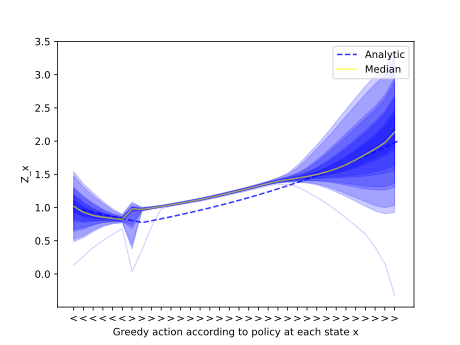
\includegraphics[scale=\munosbirdscale]{results/dt51-munos-overview}
  \end{minipage}%
  \begin{minipage}{0.49\linewidth}
    \centering
    \textsc{DEICIDE TD}\\
    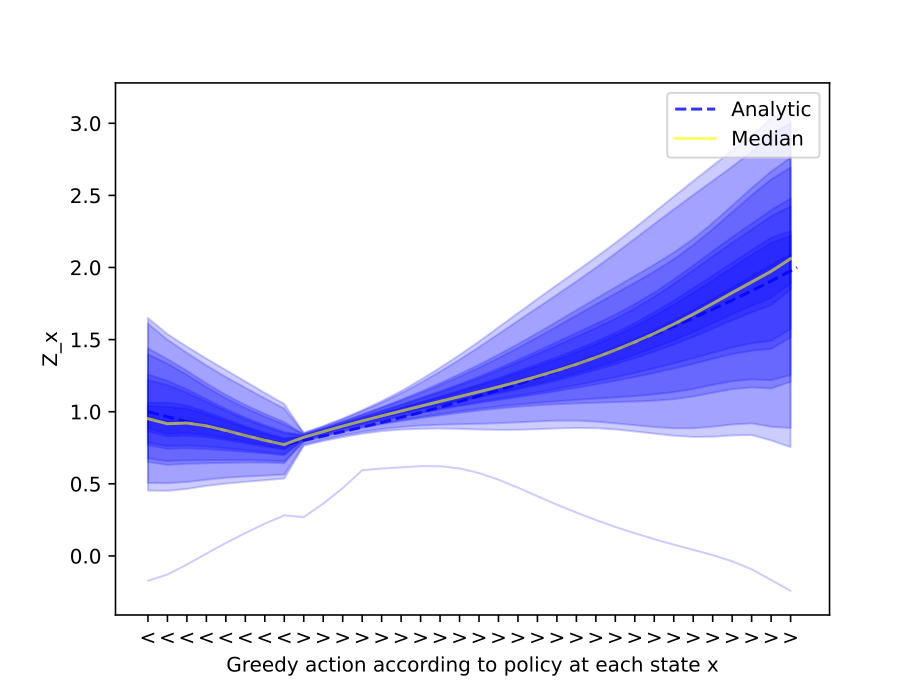
\includegraphics[scale=\munosbirdscale]{results/ct51-munos-overview}
  \end{minipage}%
  \caption{Bird's eye view of the learned return distribution
    functions}
  \label{fig:exp:munos:bird}
\end{figure}

As in the expected value RL case, we see that the median of the return
measure functions converges nicely to the ground truth in our
continuous-time algorithm, however the discrete-time algorithm is
disturbed at the point of non-differentiability. More interestingly,
the return measure function learned in the discrete-time algorithm has
some bizarre properties:
\begin{itemize}
\item The distributions are not symmetric. Since the agent only
  receives a single reward which is Gaussian-distributed, we should
  expect the return measures to be Gaussian, especially near the
  endpoints. This is not the case at all for the discrete-time
  algorithm.
\item The variance of the return measure vanishes very rapidly as
  the state moves away from the boundaries, to the point where the
  return measures are effectively deterministic in most of the state
  space. This is not the case with our continuous-time algorithm.
\item Aside from the return measures \emph{and} their medians being
  off, the the return measures also do not induce an optimal policy in
  our experiment.
\end{itemize}

We can examine some of these oddities further. Comparing the return
measures estimated near the endpoints, we observe the data shown in
Figure \ref{fig:exp:munos:bounds}.

\begin{figure}[h]
  \centering
  \newcommand{\munosscanscaledt}{0.73}
  \newcommand{\munosscanscalect}{0.73}
  \textsc{Quantile Regression TD}\\
  \begin{minipage}[t]{0.495\linewidth}
    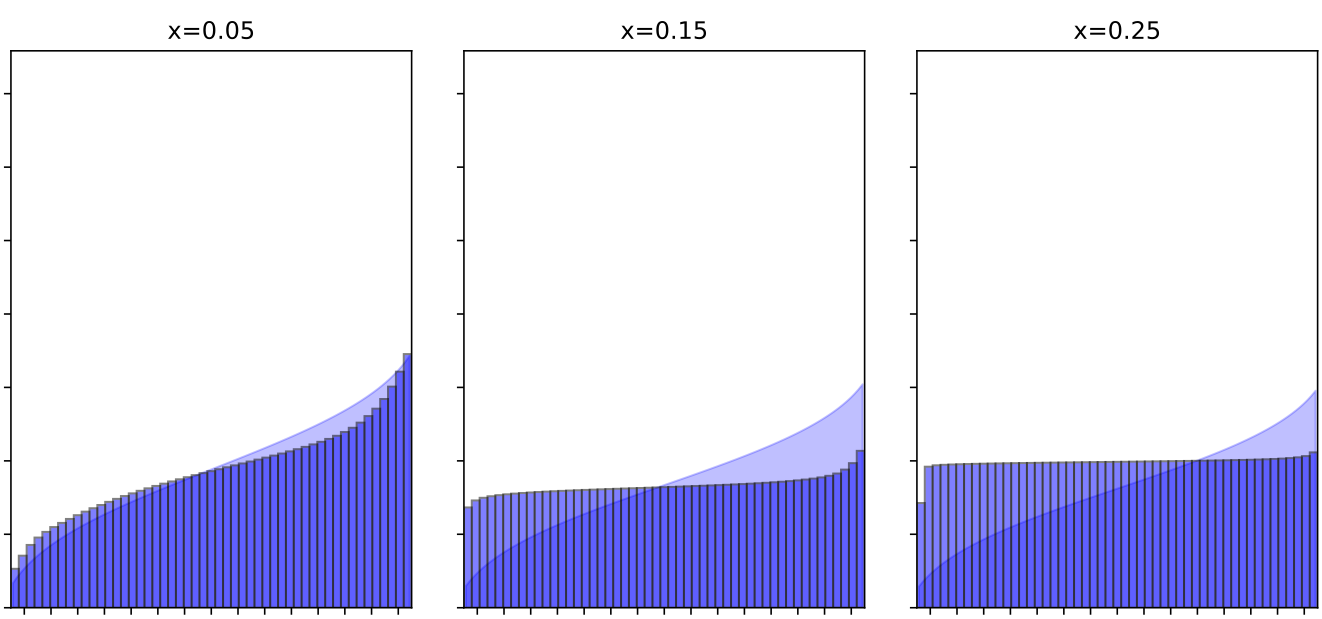
\includegraphics[scale=\munosscanscaledt]{results/dt51-munos-scan-left}
  \end{minipage}%
  \begin{minipage}[t]{0.495\linewidth}
    \centering
    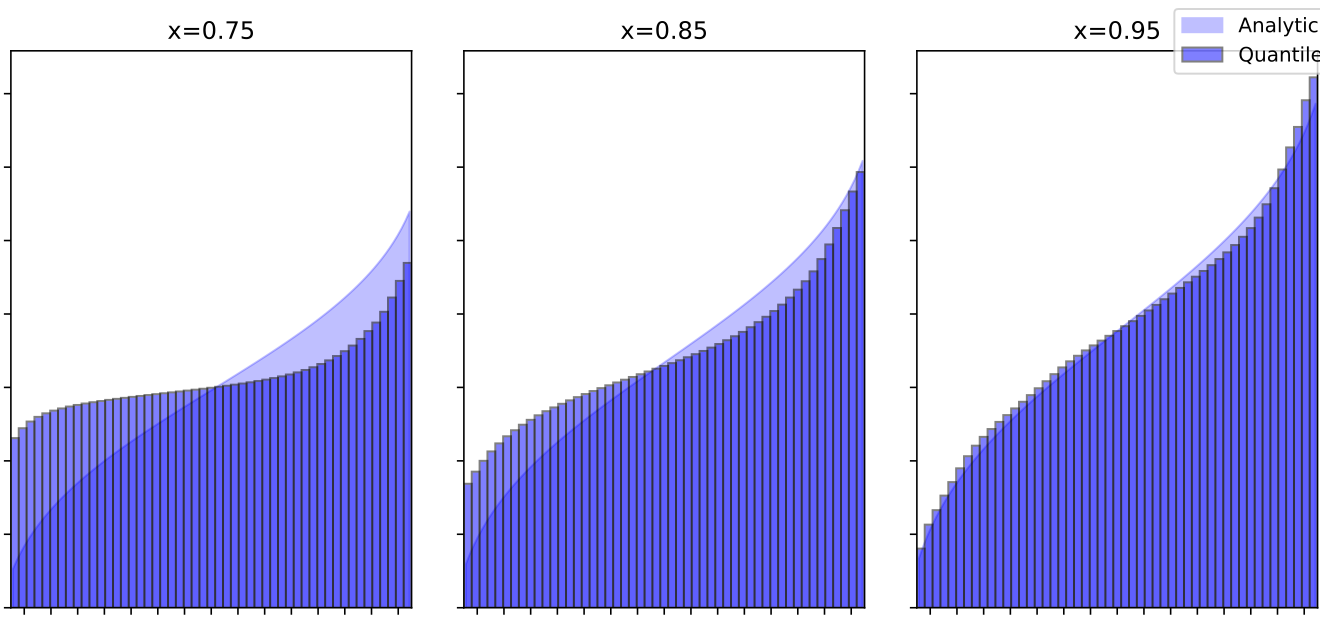
\includegraphics[scale=\munosscanscaledt]{results/dt51-munos-scan-right}
  \end{minipage}
  \textsc{DEICIDE TD}\\
  \begin{minipage}[t]{0.495\linewidth}
    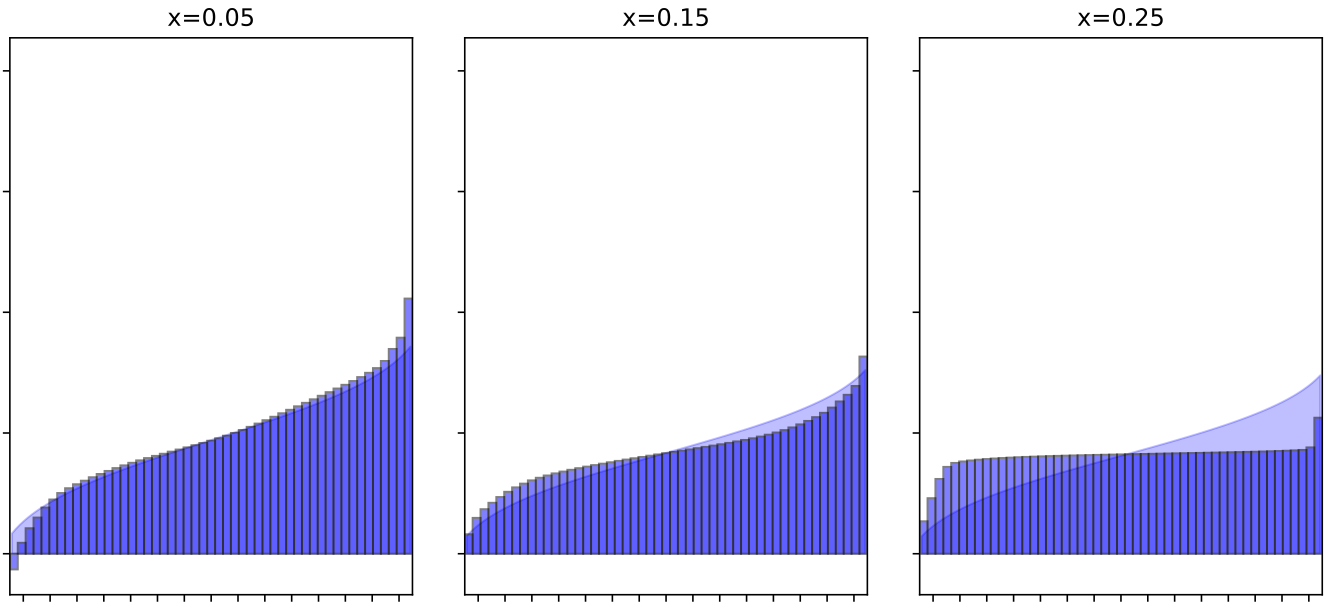
\includegraphics[scale=\munosscanscalect]{results/ct51-munos-scan-left}
  \end{minipage}%
  \begin{minipage}[t]{0.495\linewidth}
    \centering
    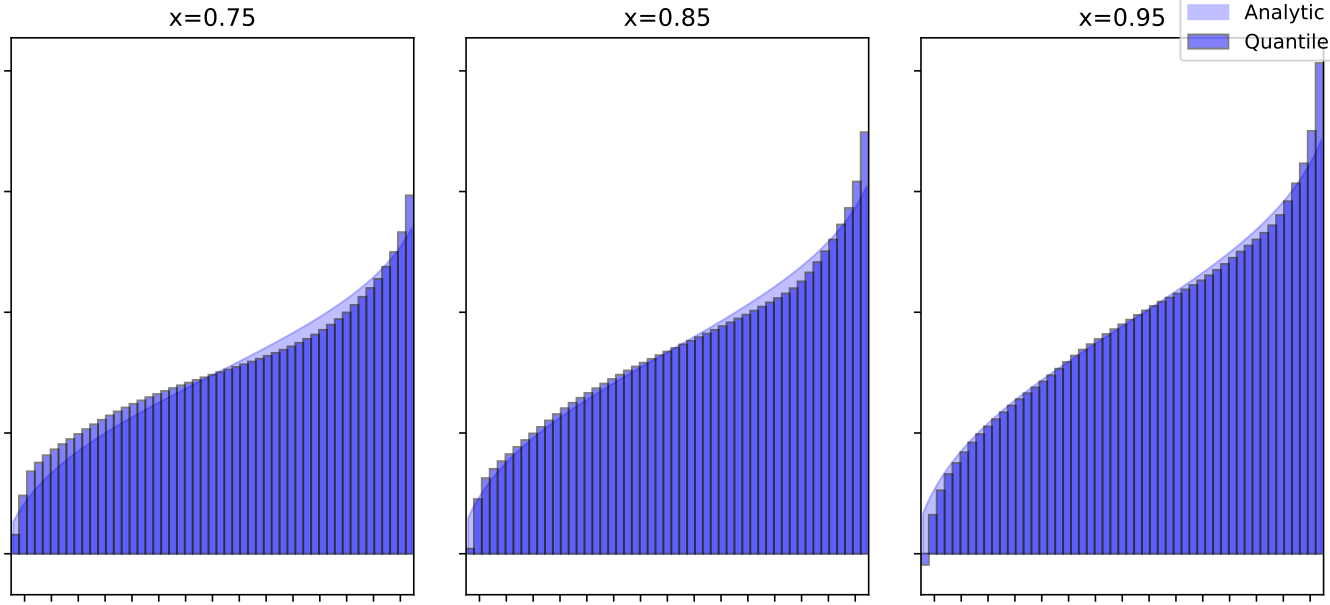
\includegraphics[scale=\munosscanscalect]{results/ct51-munos-scan-right}
  \end{minipage}
  \caption[Estimates of the return measures near the boundaries]{%
    Quantile functions learned by both algorithms near the
    boundaries. The horizontal axis is the quantile $\tau$ and the
    vertical axis is the $\tau$-quantile. The pale shaded region is
    the ground truth quantile function. The state input is indicated
    above each graph.
  }
  \label{fig:exp:munos:bounds}
\end{figure}

We see that both algorithms tend to shed variance in the interior of
the state space, however DEICIDE tends to model the full distribution
substantially better, as we expect from Figure \ref{fig:exp:munos:bird}.

\subsection{Deterministic Environments}
Recall that the analysis we presented for return distributions always
assumed that the return measures are absolutely continuous with
respect to the Lebesgue measure. A reasonable question to ask, then,
is how DEICIDE algorithms behave in deterministic environments where
the true returns have distributions $\dirac{V^\pi(\cdot)}$, since
these distributions most certainly do not satisfy this assumption.

Figure \ref{fig:exp:cartpole:deterministic} illustrates the quantiles
learned by Algorithm \ref{alg:deicide:fd} when trained on the classic
\textsc{CartPole-v0} benchmark \citep{brockman2016openai}.

\begin{figure}[h]
  \centering
  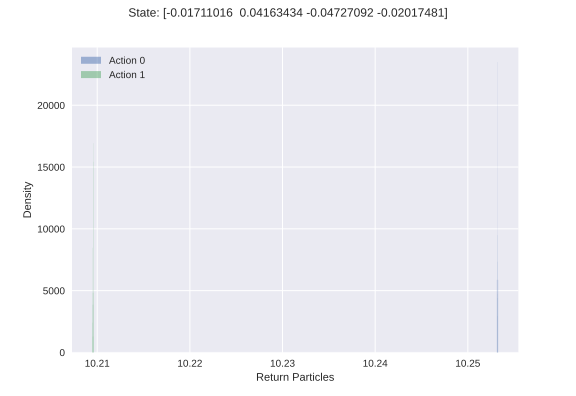
\includegraphics[scale=0.8]{results/ct51-cartpole-deterministic-returns}
  \caption[DEICIDE performance in a deterministic setting]{DEICIDE
    performance in \textsc{CartPole-v0}} 
  \label{fig:exp:cartpole:deterministic}
\end{figure}

We see that DEICIDE was able to accurately model the return
distributions as approximate Dirac measures.

\subsection{Deep DEICIDE}
Finally, we showcase the performance of DEICIDE in a continuous-time
stochastic setting. We modify the \textsc{CartPole-v0} benchmark
\citep{brockman2016openai} to create a benchmark, which we call
\textsc{NoisyContinousTimeCartPole-v0}, as follows:

\begin{itemize}
\item We sample timesteps $\tau\sim\mathsf{Exponential}(100) +
  10^{-3}$;
\item We perturb force inputs to the cart with Gaussian noise sampled
  from $\mathcal{N}(0, 1)$;
\item We provide three more actions to deal with noise: a ``NO-OP''
  action with applies no force, and a double force action in each direction.
\end{itemize}

We implement Algorithm \ref{alg:deicide:fd} with a deep neural network
estimating the $N=11$ quantile functions (and another for the target quantile
functions), as well as a deep neural network estimating the system
dynamics and trained via the reparameterization trick.

The experiment is run over several hyperparameter configurations and
random seeds, as suggested by \citet{henderson2018deep}. We see that
DEICIDE is fairly stable with respect to hyperparameter configurations
and seeds, as illustrated in Figure \ref{fig:exp:cartpole:stability}.

\begin{figure}[h]
  \centering
  \newcommand{\cartpolestabilityscale}[0]{0.34}
  \begin{minipage}{0.49\linewidth}
    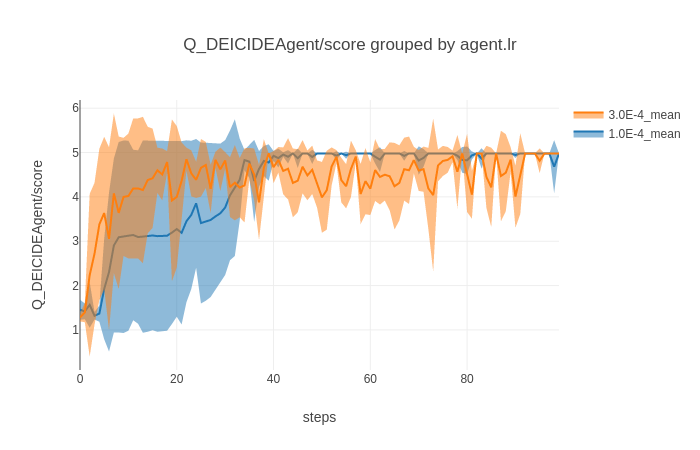
\includegraphics[scale=\cartpolestabilityscale]{results/ct-fd-cartpole-lr}
  \end{minipage}
  \begin{minipage}{0.49\linewidth}
    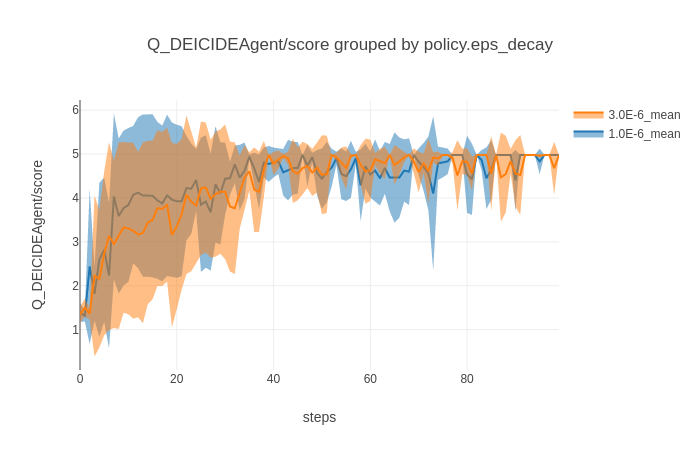
\includegraphics[scale=\cartpolestabilityscale]{results/ct-fd-cartpole-epsdecay}
  \end{minipage}
  \caption{Stability of DEICIDE with respect to hyperparameter
    configurations and random seeds}
  \label{fig:exp:cartpole:stability}
\end{figure}

Additionally, we see that the agents learned the optimal controller
very quickly. As an example, Figure
\ref{fig:exp:cartpole:returnmeasure} displays the return measure
function learned by the agent at a random initial state.

\begin{figure}[h]
  \centering
  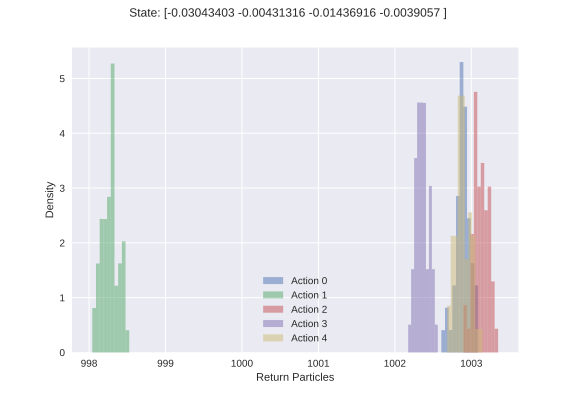
\includegraphics[scale=0.4]{results/ct51-fd-cartpole-returns}
  \caption{Return measure learned by a deep DEICIDE agent}
  \label{fig:exp:cartpole:returnmeasure}
\end{figure}

\chapter{Conclusion}
In this thesis, we studied the essentially unexplored problem of
learning return distributions for continuous-time Markov processes. We
provide theory about the characterization of return measures in the
continuous-time limit, and analyze how the tractable representation of
probability measures affect this characterization.

Based on our analysis, we discuss the implementation of 
algorithms for continuous-time distributional reinforcement learning,
and we introduce the DEICIDE framework for achieving this.
Upon testing DEICIDE implementations against some simple control
benchmarks, we observe that our continuous-time algorithm
substantially outperforms the Quantile Regression TD learning baseline
in an environment where the value function is non-differentiable, as
hypothesized.  In fact, the failure of discrete-time algorithms in
this setting was far more pronounced in the stochastic case relative
to our continuous-time implementation.

Finally, we demonstrated that DEICIDE algorithms can be endowed with
highly nonlinear function approximators such as deep neural
networks. We see that such implementations are able to accurately
learn return distribution functions in a stochastic extension of the
common \textsc{CartPole-v0} benchmark with randomly-sampled timesteps.

To conclude, the results presented in this thesis show promise for
the prospects distributional reinforcement learning in continuous
time, however lots of room is left for future work in this field. For
instance, a distributional extension of Advantage Updating
\citep{baird1993advantage} is by no means a trivial task, but may
drastically improve continuous-time distributional RL
algorithms. Moreover, an interesting future direction in this line of
work would involve studying methods of simulating and evaluating the
continuous-time performance of RL algorithms. In this thesis, we very
briefly touch on this with our experiments that sample random
timesteps. However, the distribution of the timestep duration was
essentially arbitrary and may not be a good model for such phenomena
in the real world, such as randomly-timed observations from robotic
systems with several sensors. Further investigation into such models
can potentially reveal further challenges in continuous-time RL that
could hinder the performance of RL-trained systems in the real world.

\appendix

\chapter{A Primer on Topology}\label{app:analysis}
Concepts from the field of topology are mentioned often in this
thesis. Some definitions and basic results are stated here.

\begin{definition}[Topological Space]\label{def:topology}
  A \textbf{topological space} is a pair $(X, \mathcal{O})$ consisting of a set
  $X$ and a collection $\mathcal{O}\subset 2^X$ of subsets of $X$ such
  that
  \begin{enumerate}
  \item $\emptyset\in\mathcal{O}$ and $X\in\mathcal{O}$;
  \item If $\indexedin{I}{\alpha}{U}\subset\mathcal{O}$, then
    $\bigcup_{\alpha\in I}U_\alpha\in\mathcal{O}$;
  \item If $N$ is a finite integer and
    $\indexedint{i}{N}{U}\subset\mathcal{O}$,
    then $\bigcap_{i\in[N]}U_i\in\mathcal{O}$.
  \end{enumerate}

  The set $\mathcal{O}$ is called a \textbf{topology} on $X$, and the
  elements of $\mathcal{O}$ are called \textbf{open sets}.
\end{definition}

It is only natural to ask what it means for a set to be closed.

\begin{definition}[Closed Set]
  Let $(X,\mathcal{O})$ be a topological space. A set $F\subset X$ is
  said to be \textbf{closed} if its complement is an open set.
\end{definition}

\begin{remark}
  It should be noted that openness and closedness are not mutually
  exclusive properties of sets -- in fact, by the very definition of a
  topology, the ``whole space'' and the empty set must both be
  simultaneously open and closed. Such sets are called \textbf{clopen}.
\end{remark}

The choice of the topology characterizes what it means for a function
to be continuous and what it means for a sequence to converge (among
other things).

\begin{definition}[Continuous Function]\label{def:continuity}
  Let $(X,\mathcal{O}), (Y,\mathcal{U})$ be topological spaces. A
  function $f:(X, \mathcal{O})\to(Y, \mathcal{U})$ is said to be
  continuous if its preimage of every open set $U\subset Y$ is an open
  set in $X$. That is,

  \begin{align*}
    U\in\mathcal{U}\implies\{x\in X: f(x)\in U\}\in\mathcal{O}
  \end{align*}
\end{definition}

\begin{definition}[Convergence]\label{def:convergence}
  Let $(X,\mathcal{O})$ be a topological space. A sequence
  $\indexedint{i}{N}{x}\subset X$ is said to \textbf{converge} to a
  point $x\in X$ if for every open set $U\ni x$ there exists a finite
  integer $N$ such that $\indexedint[N]{i}{\infty}{x}\subset U$.
\end{definition}

The following proposition can be verified directly.

\begin{proposition}[The Universal Topology]
  \label{pro:universal-topology}
  Let $X = \mathbf{N}$ and let
  \begin{align*}
    \mathcal{O} = \{\emptyset, X, U, X\setminus U\}
  \end{align*}
  where $U = \{4,8,15,16,23,42\}$. Then any sequence
  $\indexedint{i}{\infty}{x}\subset X$ such that
  $\indexedint[N]{i}{\infty}{x}\subset U$ converges to $42$, where $N$
  is a finite integer. For instance, the sequence $15, 16, 15, 16,
  \dots\to 42$.
\end{proposition}

\section{Metric Spaces}\label{s:metric-space}
Proposition \ref{pro:universal-topology} should be a little
alarming. Indeed, many topological spaces are quite
pathological. Usually we restrict our interests to spaces with a
little more structure, such as a spaces that can be equipped with a
meaningful notion of distance.

\begin{definition}[Metric Space]\label{def:metric-space}
  A \textbf{metric space} is a pair $(X, d_X)$ where $X$ is a set and
  $d_X:X\times X\to\mathbf{R}_+$, called a \textbf{metric} or a
  distance function, satisfies
  \begin{enumerate}
  \item (\emph{Separation of points}) For any $x,y\in X$, $d_X(x, y) = 0\iff
    x = y$;
  \item (\emph{Symmetry}) For any $x,y\in X$, $d_X(x, y) = d_X(y, x)$;
  \item (\emph{Triangle inequality}) For any $x,y,z\in X$, $d_X(x,
    z)\leq d_X(x, y) + d(y, x)$.
  \end{enumerate}
\end{definition}

A metric space is a special case of a topological space, where the
topology is understood to be the smallest topology\footnote{The
  \emph{smallest} topology conforming to some constraint is the
  intersection of all topologies that conform to the constraint.} containing all open
balls $B_r(x) = \{y\in X : d_X(x, y)<r\}$. Notably, not every
topological space has a metric structure. For instance, there is no
function on $\mathbf{N}$ with the
\hyperref[pro:universal-topology]{universal topology} that satisfies
the metric properties.

\begin{remark}
  The definitions of \hyperref[def:continuity]{continuity} and
  \hyperref[def:convergence]{convergence} on metric spaces coincide
  with those that are given in standard calculus courses.
\end{remark}

\begin{definition}[Cauchy Sequence]
  Let $(X, d)$ be a metric space. A sequence
  $\indexedint{i}{\infty}{x}\subset X$ is called a \textbf{Cauchy
    sequence} if for every $\epsilon>0$ there exists a finite integer
  $N$ such that

  \begin{align*}
    d(x_n, x_m)\leq\epsilon\qquad\forall m,n\geq N
  \end{align*}
\end{definition}

\begin{remark}
  Counterintuitively, Cauchy sequences may not converge. A sequence
  only converges (in a given topological space) if the limit lies in
  the space. For instance, the sequence
  $\indexedint{k}{\infty}{x}\subset (0,1)$ where $x_k=\frac{1}{k}$ is
  Cauchy, but its limiting value is $0$ which is not in $(0,1)$.
\end{remark}

\begin{definition}[Complete Space]\label{def:complete}
  A metric space $(X, d)$ is said to be \textbf{complete} if every
  Cauchy sequence in $X$ converges in $X$. By the previous remark, the
  set $(0,1)$ is not complete with the standard topology on the real numbers.
\end{definition}

Finally, we demonstrate a useful property of metric spaces.

\begin{lemma}[Well-behaved convergence]\label{lem:metric:convergence}
  In any metric space $(X, d)$, no sequence can converge to more than
  one point.
\end{lemma}
\begin{proof}
  Suppose $\indexedint{k}{\infty}{x}\subset X$ has limits $x, y$. Then

  \begin{align*}
    \lim_{k\to\infty}d(x_k, x) &= 0\\
  \end{align*}

  Moreover, by the triangle inequality, for any $k$ we have $d(x,
  y)\leq d(x, x_k) + d(x_k, y)$. Therefore,

  \begin{align*}
    d(x, y) &\leq \lim_{k\to\infty}d(x, x_k) + \lim_{k\to\infty}d(x_k,
              y)\\
    &= d(x_k, y)
  \end{align*}
  So if $x_k\to y$, then we must have $d(x, y) = 0$, and by the
  separation of points property this implies that $x=y$.
\end{proof}
%\label{app:analysis}
\chapter{The Basics of Measure Theory}\label{app:measure}

\newcommand{\vol}{\mathsf{Vol}}

Measure theory is a vast field of mathematical analysis that is
concerned with generalizing the notion of \emph{measure}, such as
length, area, and volume, to arbitrary spaces. For the sake of building
intuition, suppose we have a 3-dimensional sphere $S =
\{x\in\mathbf{R}^3 : \|x\|\leq r\}$ and we are interested in measuring
its volume, as well as the volume of arbitrary ``pieces'' of the
sphere. Formally, we're looking for a function $\mathsf{Vol}:2^S\to
\mathbf{R}_+$ that maps subsets of the sphere to a non-negative real
number. This function cannot just be an arbitrary function, as we
expect a volume to satisfy certain properties. For instance, we need
the following:

\begin{enumerate}
\item Emptiness has no volume: $\vol(\emptyset) = 0$;
\item For disjoint subsets $A,B\subset S$, the volume of the
  combination of $A,B$ should be equivalent to the sum of their
  original volumes: $A\cap B=\emptyset\implies\vol(A + B) = \vol(A) +
  \vol(B)$;
\item For any subset $D\subset S$, no subset of $D$ can have more
  volume than $D$: $C\subset D\implies\vol(C)\leq\vol(D)$.
\end{enumerate}

This is not particularly interesting at first glance. However, with
this definition of measure, there are some alarming consequences. In
particular, the \emph{Banach-Tarski paradox} demonstrates how one can
disassemble $S$ into a collection of pieces, and reassemble the pieces
to form two identical copies of $S$
\citep{banach1924decomposition}. Moreover, a function that
measures the length of arbitrary subsets of the real
line (according to the rules above) and assigns finite length to the interval $(0,1)$ \emph{cannot
  possibly exist} \citep{cohn2013measure}.

Interestingly, the issue lies not exactly with the rules we listed,
but with the sets we wish to measure. In short, in order to construct
a meaningful measure function, we must restrict this function to
measure only ``nice-enough'' sets. In this context, the collection of ``nice
enough'' sets is actually quite vast, and it is usually difficult to
even conceive a set that is not nice enough. This will be explained in
further detail in \S\ref{app:measure:measure}, and integration with
respect to measures will be discussed in
\S\ref{app:measure:integration}.

\section{Measurable Spaces}\label{app:measure:measure}

The distinction of sets that can and cannot be measured is formalized
by a \emph{measurable space}. Not unlike topological spaces, a
measurable space is comprised of a set with a collection of subsets,
where the subsets denote the sets that one may measure. Like the
topology of a set, the collection of measurable sets cannot be
arbitrary. Rather, it must be a \emph{$\sigma$-algebra}.

\begin{definition}[$\sigma$-algebra]\label{def:sigma-algebra}
  Let $\Omega$ be a set. A \emph{$\sigma$-algebra over $\Omega$} is a
  collection of subsets $\Sigma\subset 2^\Omega$ such that

  \begin{enumerate}
  \item $\emptyset, \Omega\in\Sigma$;
  \item $A\in\Sigma\implies A^c = \Omega\setminus A\in\Sigma$;
  \item If $\indexedint{k}{\infty}{A}$ is a countable collection of sets in
    $\Sigma$, then $\bigcup_kA_k\in\Sigma$.
  \end{enumerate}

  We occasionally refer to the \emph{smallest $\sigma$-algebra}
  containing a collection of subsets, or the $\sigma$-algebra
  \emph{generated by} this collection of subsets. For a collection of
  subsets $\mathcal{U}\subset 2^\Omega$, this $\sigma$-algebra is denoted by
  $\sigma(\mathcal{U})$ and is defined as

  \begin{align*}
    \sigma(\mathcal{U}) = \bigcap\left\{\Sigma\in 2^\Omega :
    \Sigma\text{ is a $\sigma$-algebra},\quad \mathcal{U}\subset\Sigma\right\}
  \end{align*}
\end{definition}

Essentially, the $\sigma$ algebra describes any quantities we may want
to measure. If we are able to measure the volume of $S$ and we are
able to measure the volume of $A\subset S$, then naturally we should
be able to measure the volume of $S\setminus A$. Likewise, if we can
measure the volume of a countable collection of subsets of $S$, we
should be able to measure their union. While this construction seems
rather innocuous, $\sigma$-algebras can contain exceptionally
``rough'' sets. Below, we define a family of $\sigma$-algebras that is
referred to extensively in this thesis.

\begin{definition}[Borel $\sigma$-algebra]\label{def:borel}
  Let $(X, \mathcal{O})$ be a \hyperref[def:topology]{topological
    space}. The \emph{Borel $\sigma$-algebra over $(X,\mathcal{O})$}
  (or the Borel $\sigma$-algebra over $X$ when the topology is
  implicit), denoted by $\mathscr{B}(X, \mathcal{O})$, is the
  smallest $\sigma$-algebra containing $\mathcal{O}$.
\end{definition}

\begin{definition}[Measurable Space]\label{def:measurable-space}
  A \emph{measurable space} is a pair $(\Omega, \Sigma)$ where
  $\Omega$ is a set and $\Sigma$ is a $\sigma$-algebra over $\Omega$.
\end{definition}

We are finally able to formalize the concept of a measure.

\begin{definition}[Measure]\label{def:measure}
  Let $(\Omega, \Sigma)$ be a measurable space. A \emph{measure} on
  $(\Omega,\Sigma)$ is a function $\mu:\Sigma\to\mathbf{R}_+$ such
  that

  \begin{enumerate}
  \item $\mu(\emptyset) = 0$;
  \item $A\subset B\implies \mu(A)\leq\mu(B)$;
  \item If $\indexedint{k}{\infty}{A}$ is a countable collection of disjoint
    sets in $\Sigma$ (so $i\neq j\implies A_i\cap A_j=\emptyset$),
    then
    \begin{align*}
      \mu\left(\bigcup_{k=1}^\infty A_k\right) = \sum_{k=1}^\infty \mu(A_k)
    \end{align*}
  \end{enumerate}

  A tuple $(\Omega, \Sigma, \mu)$ is called a \emph{measure space}.
\end{definition}

Taking a step back to the examples above, it is known that there is no
measure on the measurable space $(\mathbf{R}, 2^{\mathbf{R}})$ that
assigns finite measure to $(0,1)$, and matter can be created out of
thin air if we can break apart objects into any subset of space.

A very important result in measure theory is the existence of a measure
space over $\mathbf{R}$ that assigns the measure $|b - a|$ to subsets
of the form $(a, b), [a, b], (a, b], [a, b)$. This measure is called
\emph{the Lebesgue measure}\label{def:lebesgue}, and it is the only
measure satisfying the mentioned property. See
\citet{cohn2013measure}, or any textbook on measure theory, for more
rigorous details.

Finally, we'll define the class of functions that preserve
measure-theoretic properties.

\begin{definition}[Measurability]
  Let $(\Omega, \Sigma), (\Omega', \Sigma')$ be measurable spaces. A
  function $f:(\Omega, \Sigma)\to(\Omega', \Sigma')$ is said to be
  \emph{measurable} if the preimage of every $\Sigma'$-measurable set
  $A$ through $f$ is $\Sigma$-measurable.
\end{definition}

It can quickly be verified that the composition of measurable
functions is itself a measurable function
\citep{cohn2013measure}. Therefore, we can define measures through a
change of variables, assuming the mapping between variables is
measurable.

\begin{definition}[Pushforward Measure]
  Let $(\Omega, \Sigma, \mu)$ be a measure space, and let $(\Omega',
  \Sigma')$ be a measurable space. For any measurable function
  $f:(\Omega, \Sigma)\to(\Omega',\Sigma')$, the \emph{pushforward of $f$
    through $\mu$}, denoted $\pushforward{f}{\mu}$, is a measure on
  $(\Omega', \Sigma')$ given by

  \begin{align*}
    \pushforward{f}{\mu} = \mu\circ f^{-1}
  \end{align*}

  where $f^{-1}$ is the preimage of $f$.
\end{definition}

\subsection{Measure-theoretic Probability Theory}\label{s:app:measure:probability}
A natural application of this formalism, aside from measurements of
geometric properties, is probability. In fact, we can formalize
probability very easily as a measure space.

\begin{definition}[Probability Space]\label{def:probability}
  A \emph{probability space} is a measure space $(\Omega, \Sigma,
  \mu)$ where $\mu(\Omega) = 1$.
\end{definition}

Occasionally, in the context of probability, the set $\Omega$ is
called the \emph{sample space}, the $\sigma$-algebra $\Sigma$ is
called the \emph{event space}, and the measure $\mu$ is called a
\emph{probability measure}.

Moreover, we can use the language of measure theory to formalize the
concept of a random variables.

\begin{definition}[Random Variable]\label{def:random-variable}
  Let $(\Omega, \Sigma, \mu)$ be a probability space, and let $A$ be
  an arbitrary set. A \emph{random variable} on this space is a
  function $Y:\Sigma\to A$.
\end{definition}

For a given measure space $(\Omega, \Sigma, \mu)$, a property is said
to hold \emph{$\mu$-almost everywhere} (or simply ``almost
everywhere'' when the measure is implicit) if the property holds on
all of $\Omega$, except for possibly a set $A$ with $\mu(A) = 0$. When
$\mu$ is a probability measure, it is sometimes said that the property
holds \emph{almost surely}.

\section{Integration}\label{app:measure:integration}
A measure can be thought of as an arbitrary method of assigning weight
or density to a space. As such, the notation of integration can be
formulated in terms of measures. In this section, a brief overview of
this type of integration, known as Lebesgue integration, and its properties will be given.

We'll consider a measure space $(\Omega, \Sigma, \mu)$. In order to
construct an integral, we'll begin by defining the integral on a
simple class of functions, aptly called the \emph{simple functions}.

\begin{definition}[Simple Function]\label{def:simple-function}
  A \emph{simple function} $f$ is a function of the form

  \begin{align*}
    f(x) &= \sum_{i=1}^n\alpha_i\chi_{A_i}(x)
  \end{align*}

  where $\alpha_i\in\mathbf{R}$ and $\indexedint{i}{n}{A}$ is a finite
  collection of measurable sets.
\end{definition}

It is easy to verify that the sum and product of simple functions are
both simple functions. The notion of integration of a simple function
$f$ with respect to a measure is fairly intuitive. We define

\begin{align*}
  \int f(x)d\mu &= \sum_{i=1}^n\alpha_i\mu(A_i)\qquad f = \sum_{i=1}^n\alpha_i\chi_{A_i}
\end{align*}

By linearity, it clearly follows that the Lebesgue integral restricted
to simple functions is linear. The Lebesgue integral of measurable
functions $f$ is given by

\begin{align*}
  \int fd\mu &= \sup\left\{\int sd\mu : s\text{ is a simple function}\right\}
\end{align*}

It is well known that the Lebesgue integral is linear over all
measurable functions, and it is well defined. Moreover, it is known
that the Lebesgue integral with respect to the Lebesgue measure agrees
with the Riemann-Stieltjes integral on all integrable functions.

\subsection{Convergence
  Theorems}\label{s:app:measure:integration:convergence}
In this section, we'll simply state some commonly known convergence
properties of the Lebesgue integral. See \citet{cohn2013measure} for
further details.

\begin{theorem}[The Monotone Convergence Theorem]\label{thm:monotone-convergence}
  Let $(\Omega, \Sigma, \mu)$ be a measure space and let
  $\indexedint{i}{\infty}{f}$ be a sequence of $[0,\infty]$-valued
  $\Sigma$-measurable functions. Suppose that for all $f_i\leq f_j$
  for all $i\leq j$, and that $\lim_{i\to\infty}f_i(x) = f(x)$ for
  almost every $x\in X$. Then $\int fd\mu = \lim_{i\to\infty}\int f_id\mu$.
\end{theorem}

\begin{theorem}[The Dominated Convergence
  Theorem]\label{thm:dominated-convergence}
  Let $(\Omega, \Sigma, \mu)$ be a measure space, $g$ a
  $[0,\infty]$-valued integrable function on $\Omega$, and
  $\indexedint{n}{\infty}{f}$ a collection of $\Sigma$-measurable
  functions where $\lim_{n\to\infty}f_n(x) = f(x)$ almost
  everywhere. If $|f_n(x)|\leq g(x)$ almost everywhere for each $n$,
  then $\indexedint{n}{\infty}{f}$ and $f$ are integrable, and $\int f(x) =
  \lim_{n\to\infty}\int f_nd\mu$ almost everywhere.
\end{theorem}
%\label{app:measure}
\chapter{Tools from the Theory of Stochastic Processes}\label{app:stochastic}
This appendix will survey some concepts from the theory of stochastic processes
that are useful in the developments of this thesis. This theory tends to be
quite technical, and one should be comfortable with the concepts of Appendices
\ref{app:analysis} and \ref{app:measure} before proceeding.

\section{Some Special Classes of Stochastic Processes}
\subsection{Measurable, Adapted, and Progressive Processes}\label{app:adapted}
When dealing with stochastic processes, there are a few properties that we
generally desire in order for us to be able to analyze them nicely. The most
common examples will be summarized here. These definitions are due to
\citet{le2016brownian}.

For the following definitions, we will fix a
\hyperref[def:probability-space]{probability space} $(\Omega, \mathcal{F},
\Pr)$, and we will consider a stochastic process
$\indexedabove{t}{X}\subset\mathcal{X}$, where $(\mathcal{X}, \Sigma)$ is a
\hyperref[def:measurable-space]{measurable space}..

\begin{definition}[Measurable Process]\label{def:process:measurable}
  The process
  $\indexedabove{t}{X}\subset \mathcal{X}$
  is said to be
  \emph{measurable} if $(\omega, t)\mapsto X_t(\omega)$ is a measurable map on
  $\Omega\times\mathbf{R}_+$ with respect to the smallest $\sigma$-algebra on
  $\mathscr{B}(\mathbf{R}_+)\times\mathcal{F}$.
\end{definition}

For the remainder of the definitions, we will also consider a
\hyperref[def:filtration]{filtration} (see Definition \ref{def:filtration})
$\indexedabove{t}{\mathcal{F}}$ making $(\Omega, \mathcal{F},
\indexedabove{t}{\mathcal{F}},\Pr)$ a filtered probability space.

\begin{definition}[Adapted Process]\label{def:process:adapted}
  The process $\indexedabove{t}{X}\subset\mathcal{X}$ is \emph{adapted} if $X_t$
  is $\mathcal{F}_t$-measurable for every $t\geq 0$.
\end{definition}

\begin{definition}[Progressive Process]\label{def:process:progressive}
  The process $\indexedabove{t}{X}\subset\mathcal{X}$ is \emph{progressive}
  (or \emph{progressively measurable}) if $(\omega, s)\mapsto X_t(\omega)$ is
  measurable on $\Omega\times[0,t]$ with respect to the smallest
  $\sigma$-algebra on $\mathcal{F}_t\times\mathscr{B}([0,t])$ for each $t\geq
  0$.
\end{definition}

\subsection{Martingales}\label{app:martingale}
\begin{definition}[Martingales, \cite{rogers1994diffusions}]
  \label{def:martingale}
  A \textbf{martingale} (relative to a given
  \hyperref[def:filtration]{filtration} $(\mathcal{F}_t)_{t\geq 0}$)
  is a stochastic process $(M_t)_{t\geq 0}$ where 
  $M_t\in L^1$ and
  \begin{equation}
    \label{eq:martingale:property}
    M_s = \ConditionExpect{M_t}{\mathcal{F}_s}\qquad 0\leq s \leq t
  \end{equation}

  Equation \eqref{eq:martingale:property} is referred to as ``the
  martingale property''. If the equality in
  \eqref{eq:martingale:property} is instead $\geq$ (resp. $\leq$), $(M_t)_{t\geq 0}$
  is called a \textbf{supermartingale} (resp. \textbf{submartingale}).
\end{definition}

\begin{definition}[Local Martingales, \cite{le2016brownian}]
  \label{def:local-martingale}
  A \textbf{local martingale} is a stochastic process $(M_t)_{t\geq
    0}$ for which there exists a sequence of nondecreasing
  \hyperref[def:stopping-time]{stopping times} $(T_n)_{n=1}^\infty$
  such that $M^{T_n} = (M_{t\land T_n})_{t\geq 0}\in L^1$ is a martingale.
\end{definition}

\begin{definition}[Semimartingales, \cite{le2016brownian}]\label{def:semimartingale}
  \label{def:semimartingale}
  A \textbf{semimartingale} is a random process $(X_t)_{t\geq 0}$ such
  that $X_t = A_t + M_t$ for each $t\geq 0$, where $(A_t)_{t\geq 0}$
  is a \hyperref[app:finite-variation]{finite variation process} and
  $(M_t)_{t\geq 0}$ is a local martingale.
\end{definition}

\subsection{Finite Variation Processes}\label{app:finite-variation}
\begin{definition}[Finite Variation Function, \cite{le2016brownian}]
  Let $T\geq 0$. A continuous function $a : [0,T]\to\mathbf{R}$ with
  $a(0) = 0$ is said to have \textbf{finite variation} if there exists
  a signed measure $\mu$ on $[0,T]$ such that $a(t) = \mu([0,t])$ for
  any $t\in [0,T]$.
\end{definition}

A finite variation process is a process whose regularity is given by
finite variation sample paths, as formalized in the next definition.

\begin{definition}[Finite Variation Process, \cite{le2016brownian}]
  A process $(A_t)_{t\geq 0}$ is called a \textbf{finite variation
    process} if all of its sample paths are finite variation functions
  on $\mathbf{R}_+$.
\end{definition}

The following processes generalize the notion of covariance of random variables
to stochastic processes, and appear frequently in important stochastic calculus
theorems. Their definitions are given by \citet{le2016brownian}.

\begin{definition}[Quadratic Variation]\label{def:quadratic-variation}
  Let $\indexedabove{t}{M}$ be a \hyperref[def:local-martingale]{local
  martingale}. The \emph{quadratic variation} of $\indexedabove{t}{M}$,
  denoted $\indexedabove{t}{[M,M]}$, is the unique increasing process such
  that $(M^2_t - [M,M]_t)_{t\geq 0}$ is a local martingale.
\end{definition}

\begin{remark}
  The existence and uniqueness of the quadratic variation is shown by
  \citet[Theorem 4.9]{le2016brownian}.
\end{remark}

\begin{definition}[The Bracket of Local Martingales]\label{def:bracket}
  Let $\indexedabove{t}{M},\indexedabove{t}{N}$ be local martingales. The
  \emph{bracket} of $M,N$, denoted $\indexedabove{t}{[M,N]}$ is the finite
  variation process $\indexedabove{t}{[M,N]}$ given by
  \begin{align*}
    [M,N]_t &= \frac{1}{2}\bigg([M+N,M+N]_t - [M,M]_t - [N,N]_t\bigg)
  \end{align*}
\end{definition}

\section{\Ito's Lemma}
\Ito's Lemma is a very powerful tool in the analysis of stochastic
processes. It can be thought of as a stochastic analog to Taylor's theorem.

\begin{theorem}[\Ito's Lemma, \cite{le2016brownian}]\label{app:ito}
  Let $(X^i)_{i=1}^p$ be real valued
  \hyperref[def:semimartingale]{semimartingales} and let $f\in
  C^2(\mathbf{R})$. Let $\mathbf{X}_t = (X_t^1,\dots,X_t^p)$. Then, for every $t\geq 0$,

  \begin{equation}
    \begin{aligned}
    \label{eq:ito}
    f(\mathbf{X}_t) = f(\mathbf{X}_0) +
    \sum_{i=1}^p\int_0^t\partialderiv{f}{x^i}(\mathbf{X}_s)dX_s^i +
    \frac{1}{2}\sum_{i=1}^p\sum_{j=1}^p\int_0^t\frac{\partial^2f}{\partial
      x_i\partial x_j}(\mathbf{X}_s)d[X^i, X^j]_s
    \end{aligned}
  \end{equation}
\end{theorem}

\section{The Feynman-Kac Formula}\label{app:feynman-kac}
We make use of the following formulation of the \emph{Feynman-Kac
  formula}, as illustrated in \citet[Exercise 6.26]{le2016brownian}.

\begin{theorem}\label{thm:feynman-kac}
  Let $\indexedabove{t}{X}$ be a
  \hyperref[def:fd]{Feller-Dynkin} process in a space $\mathcal{X}$
  and let $v\in C_0(\mathcal{X})$. Define for any $x\in\mathcal{X}$
  and $\phi$ a bounded and measurable function over $\mathcal{X}$ the
  transition semigroup $\indexedabove{t}{Q^\star}$ where

  \begin{align*}
    Q_t^\star\phi(x) &= \ConditionExpect{\phi(X_t)\exp\left(-\int_0^tv(X_s)ds\right)}{X_0=x}
  \end{align*}

  If $\indexedabove{t}{X}$ admits an infinitesimal generator
  $\mathscr{L}$ and $\phi\in\mathcal{D}({\mathscr{L}})$, then

  \begin{equation}
    \label{eq:feynman-kac:generator}
    \frac{d}{dt}Q_t^\star\phi\rvert_{t=0} = \mathscr{L}\phi - v\otimes\phi
  \end{equation}
\end{theorem}

\begin{remark}
  The Feynman-Kac formula can be seen as the
  \hyperref[thm:kbe]{Kolmogorov Backward Equation} with an
  ``integrating factor''. Effectively, the Feynman-Kac formula
  allows us to identify solutions of PDEs of the form

  \begin{align*}
    \partialderiv{u}{t} &= - \mathscr{L}u + v\otimes\phi
  \end{align*}

  with conditional expectations of diffusion processes.
\end{remark}

%\label{app:stochastic}
\chapter{Tempered Distributions}
A recurring concept in many areas of mathematics, physics, and engineering is
that of \emph{generalized functions}, known as \emph{distributions}\footnote{Not
  to be confused with probability distributions.}. One such example is the Dirac
  delta. Distributions are particularly helpful at formally describing weakened solutions
  to PDEs by objects that may not be functions.

In this thesis, we will make use of the class of \emph{tempered} distributions,
whose definition will be given in this appendix. For more details, refer to
\citet{lax2002functional}.

\begin{definition}[Schwartz Class]
  Let $X$ be a normed space. A \emph{Schwartz class} is a class $\mathcal{S}$ of rapidly decaying-smooth
  functions,

  \begin{align*}
    \mathcal{S} = \left\{f\in C^\infty(X; \mathbf{R}) : \sup_{x\in X}(1 +
    \|x\|^k)|f^{(m)}(x)|<\infty\quad\forall k,m\in\mathbf{N}\right\}
  \end{align*}
\end{definition}

\begin{definition}[Tempered Distribution]\label{def:tempered-distribution}
  A tempered distribution is an element of the topological dual\footnote{The
    dual of a normed space is the set of all continuous, linear functionals on
    that space.} $\mathcal{S}'$
  of the Schwartz class $\mathcal{S}$.
\end{definition}

\begin{remark}
  The Dirac delta is the operator $\delta$ such that $\langle\delta, \phi\rangle
  = \phi(0)$. Clearly $\delta$ is linear, and since it is bounded,
  it is continuous. Therefore $\delta$ is indeed a tempered distribution.
\end{remark}

Tempered distributions admit a notion of differentiability, which can be used to
define ``distributional" solutions to PDEs.

\begin{definition}[Distributional
  Derivative]\label{def:distributional-derivative}
  Let $\mathcal{S}$ be a Schwartz class and $\psi\in\mathcal{S}'$ a tempered
  distribution. Then $\psi$ has a distributional derivative if there exists a
  tempered distribution $\psi'$ for which

  \begin{align*}
    \langle \psi', \phi\rangle &= -\langle\psi,
    \phi'\rangle\qquad\forall\phi\in\mathcal{S},
  \end{align*}

  and $\psi'$ is called the distributional derivative of $\psi$.
\end{definition}

\begin{definition}[Distributional Solutions of Hamilton-Jacobi
  PDEs]\label{def:distributional-solution}
  Consider the following PDE,
  \begin{equation}\label{eq:distributional-solution:pde}
    \partialderiv{u}{t} = f\circ u + \langle\nabla u, g\rangle +
    \quadraticform{h}{\hessian{y}u}
  \end{equation}

  where $u\in C^2(\mathbf{R}_+\times\mathcal{Y};\mathbf{R})$ for a normed space
  $\mathcal{Y}$.

  Then $\psi\in\mathcal{S}'$ is said to be a \emph{distributional solution} to
  \eqref{eq:distributional-solution:pde} if

  \begin{align*}
    &\int_0^\infty\int_{\mathcal{Y}}\phi(t, y)\left(f(\psi(y)) -
      \partialderiv{}{t}\psi(y)\right)dydt\\
    &\qquad=\int_{0}^\infty\int_{\mathcal{Y}}\bigg[\langle \psi(y)g(y), \nabla_y\phi(t,
    y)\rangle - \quadraticform{h(y)}{\psi(y)\hessian{y}\phi(t,
    y)}\bigg]dydt
  \end{align*}

  for every test function $\phi\in\mathcal{S}$. This is justified by simply multiplying both sides of
  \eqref{eq:distributional-solution:pde} by the test function, integrating over
  $\mathbf{R}_+\times\mathcal{Y}$, and substituting gradient terms of $\psi$
  with respect to its distributional derivative.
\end{definition}
\label{app:distributions}
\bibliographystyle{plainnat}
\bibliography{sources}
\end{document}
